\RequirePackage{amsmath}
\RequirePackage{fix-cm}
\documentclass[deutsch]{svmono}

\def\ColoredLinks{}
%%%%%%%%%%%%%%%%%%%%%%%%%%%%%%%%%%%%%%%%%%%
% Alexanders Standardmacros - Version 3.0 %
%%%%%%%%%%%%%%%%%%%%%%%%%%%%%%%%%%%%%%%%%%%





%%%%%%%%%%%%%%%%%%%%%%%%%%%%%%%%%%%%%%%%%%%%%%%%
%  Farben für Links definieren                 %
%%%%%%%%%%%%%%%%%%%%%%%%%%%%%%%%%%%%%%%%%%%%%%%%

\ifdefined\ColoredLinks
  \def\linkColorLinkR{0}
  \def\linkColorLinkG{0}
  \def\linkColorLinkB{0.55}
	\def\linkColorCiteR{0}
  \def\linkColorCiteG{0}
  \def\linkColorCiteB{0.55}
	\def\linkColorUrlR{0}
  \def\linkColorUrlG{0}
  \def\linkColorUrlB{0.55}
\else
  \def\linkColorLinkR{0}
  \def\linkColorLinkG{0}
  \def\linkColorLinkB{0}
	\def\linkColorCiteR{0.3}
  \def\linkColorCiteG{0.3}
  \def\linkColorCiteB{0.3}
	\def\linkColorUrlR{0}
  \def\linkColorUrlG{0}
  \def\linkColorUrlB{0}
\fi





%%%%%%%%%%%%%%%%%%%%%%%%%%%%%%%%%%%%%%%%%%%%%%%%
%  Packages einbinden                          %
%%%%%%%%%%%%%%%%%%%%%%%%%%%%%%%%%%%%%%%%%%%%%%%%

%\usepackage{makeidx} - unterschägt manchmal Einträge
\usepackage{imakeidx} % Speziellen Features eigentlicht nicht verwendet, aber hat die makeidx-Fehler nicht
\usepackage[utf8]{inputenc}
\usepackage{amssymb}
\usepackage[ngerman]{babel}
\usepackage{epsf}
\usepackage[dvips]{rotating}
\usepackage{amsmath,amsfonts}
\usepackage[amsmath,thmmarks,noconfig]{ntheorem}
\usepackage{nameref}
\usepackage{hycolor}
\usepackage{hyperxmp}
\usepackage{hyperref}
\hypersetup{pdfauthor={Alexander Herzog},
            pdftitle={Warteschlangensimulator - Kurzeinführung},
            %pdfsubject={},
            %pdfkeywords={},
            pdfproducer={LaTeX},
            pdfcreator={pdfLaTeX},
						pdfcopyright={Copyright Alexander Herzog},
						pdfcontactcity={Clausthal-Zellerfeld},
						pdfcontactpostcode={38678},
						pdfcontactcountry={Deutschland},
						pdfcontactemail={alexander.herzog@tu-clausthal.de},
						pdfcontacturl={https://www.simzentrum.de,https://www.tu-clausthal.de},
						pdflang={de},
						bookmarksnumbered,
						colorlinks=true,
						filecolor=[rgb]{0,0,0},  % \href-Links nicht hervorheben
						linkcolor=[rgb]{\linkColorLinkR,\linkColorLinkG,\linkColorLinkB},
						citecolor=[rgb]{\linkColorCiteR,\linkColorCiteG,\linkColorCiteB},
						urlcolor=[rgb]{\linkColorUrlR,\linkColorUrlG,\linkColorUrlB} %\url{}, nur für E-Mail-Link genutzt
					}
\expandafter\def\expandafter\UrlBreaks\expandafter{\UrlBreaks
  \do\a\do\b\do\c\do\d\do\e\do\f\do\g\do\h\do\i\do\j
  \do\k\do\l\do\m\do\n\do\o\do\p\do\q\do\r\do\s\do\t
  \do\u\do\v\do\w\do\x\do\y\do\z\do\A\do\B\do\C\do\D
  \do\E\do\F\do\G\do\H\do\I\do\J\do\K\do\L\do\M\do\N
  \do\O\do\P\do\Q\do\R\do\S\do\T\do\U\do\V\do\W\do\X
  \do\Y\do\Z}
\usepackage{float}
\usepackage{fancyvrb}
\restylefloat{figure}
\restylefloat{table}
\usepackage{sectsty}
%\allsectionsfont{\fontfamily{cmss}\selectfont} - das führt zu Type 3 Fonts
\allsectionsfont{\sffamily\selectfont}
\usepackage{framed}
\usepackage[toc,page]{appendix}
\renewcommand\appendixname{Anhang}
\let\appendixtocname\appendixname\let\appendixpagename\appendixname
\usepackage[T1]{fontenc} % aus der pdf kopierbare Umlaute
\usepackage{eurosym}
\usepackage{longtable}

\usepackage{graphicx}
\usepackage[export]{adjustbox}




%%%%%%%%%%%%%%%%%%%%%%%%%%%%%%%%%%%%%%%%%%%%%%%%
%  Rotierte Tabellenüberschriften              %
%%%%%%%%%%%%%%%%%%%%%%%%%%%%%%%%%%%%%%%%%%%%%%%%

\usepackage{adjustbox}
\usepackage{array}
\usepackage{booktabs}
\usepackage{multirow}

\newcolumntype{R}[2]{%
    >{\adjustbox{angle=#1,lap=\width-(#2)}\bgroup}%
    l%
    <{\egroup}%
}
\newcommand*\rot{\multicolumn{1}{|R{90}{1em}|}}





%%%%%%%%%%%%%%%%%%%%%%%%%%%%%%%%%%%%%%%%%%%%%%%%
%  Symbole definieren                          %
%%%%%%%%%%%%%%%%%%%%%%%%%%%%%%%%%%%%%%%%%%%%%%%%

\newcommand{\setH}{\mathbb{H}}
\newcommand{\setC}{\mathbb{C}}
\newcommand{\setR}{\mathbb{R}}
\newcommand{\setQ}{\mathbb{Q}}
\newcommand{\setZ}{\mathbb{Z}}
\newcommand{\setN}{\mathbb{N}}
\newcommand{\comp}{\complement}
\newcommand{\Umg}{{\cal U}}

\newcommand{\calA}{{\cal A}}
\newcommand{\calB}{{\cal B}}
\newcommand{\calC}{{\cal C}}
\newcommand{\calD}{{\cal D}}
\newcommand{\calE}{{\cal E}}
\newcommand{\calF}{{\cal F}}
\newcommand{\calG}{{\cal G}}
\newcommand{\calH}{{\cal H}}
\newcommand{\calI}{{\cal I}}
\newcommand{\calJ}{{\cal J}}
\newcommand{\calK}{{\cal K}}
\newcommand{\calL}{{\cal L}}
\newcommand{\calM}{{\cal M}}
\newcommand{\calN}{{\cal N}}
\newcommand{\calO}{{\cal O}}
\newcommand{\calP}{{\cal P}}
\newcommand{\calQ}{{\cal Q}}
\newcommand{\calR}{{\cal R}}
\newcommand{\calS}{{\cal S}}
\newcommand{\calT}{{\cal T}}
\newcommand{\calU}{{\cal U}}
\newcommand{\calV}{{\cal V}}
\newcommand{\calW}{{\cal W}}
\newcommand{\calX}{{\cal X}}
\newcommand{\calY}{{\cal Y}}
\newcommand{\calZ}{{\cal Z}}

\def\arccot{\mathop{\rm arccot}}
\def\Arcoth{\mathop{\rm Arcoth}}
\def\Arsinh{\mathop{\rm Arsinh}}
\def\Artanh{\mathop{\rm Artanh}}
\def\Arcosh{\mathop{\rm Arcosh}}

\def\d{{\rm d}}
\def\dx{\d x}
\def\dy{\d y}
\def\dz{\d z}
\def\dt{\d t}
\def\euler{\mathrm{e}}

\def\id{{\rm id}}
\def\Kern{{\rm Kern}}

\def\ra{\Rightarrow}

\def\oversym#1#2{\mathop{#1}\limits^{#2}}
\def\Inneres#1{\oversym{#1}\circ}


\def\TO#1{\oversym\longrightarrow{#1}}
\def\RA#1{\oversym\Longrightarrow{#1}}
\def\IFF#1{\oversym\iff{#1}}
\def\gleich#1{\oversym={#1}}

\def\oBdA{o.\,B.\,d.\,A.\ }

\renewcommand{\qed}{\begin{flushright} $\square$ \end{flushright}}

\def\Definition#1{{\bf #1}}

\def\E{{\bf E}}
\def\Var{{\bf Var}}
\def\Std{{\bf Std}}
\def\CV{{\bf CV}}
\def\SCV{{\bf SCV}}





%%%%%%%%%%%%%%%%%%%%%%%%%%%%%%%%%%%%%%%%%%%%%%%%
%  Umgebungen definieren                       %
%%%%%%%%%%%%%%%%%%%%%%%%%%%%%%%%%%%%%%%%%%%%%%%%

%\theoremstyle{changebreak}
%\theoremheaderfont{\normalfont\bfseries}
%\theoremseparator{:}
%\theoremsymbol{}
%\newtheorem{definition}{Definition}[chapter]
%\newtheorem{satz}[definition]{Satz}
%\newtheorem{hilfssatz}[definition]{Hilfssatz}
%\newtheorem{lemma}[definition]{Lemma}
%\newtheorem{beispiel}[definition]{Beispiel}
%\newtheorem{beispiele}[definition]{Beispiele}
%\newtheorem{bezeichnung}[definition]{Bezeichnung}
%\theorembodyfont{\rmfamily}
%\newtheorem{bemerkung}[definition]{Bemerkung}
%\newtheorem{vereinbarung}[definition]{Vereinbarung}
%\newtheorem{folgerung}[definition]{Folgerung}
%\theoremheaderfont{\normalfont\bfseries}
%\theoremstyle{nonumberchangebreak}
%\theorembodyfont{\rmfamily}
%\theoremsymbol{$\blacksquare$}
%\newtheorem{beweis}{Beweis}
%\theoremsymbol{}





%%%%%%%%%%%%%%%%%%%%%%%%%%%%%%%%%%%%%%%%%%%%%%%%
%  Standard epsilon durch schöneres ersetzen   %
%%%%%%%%%%%%%%%%%%%%%%%%%%%%%%%%%%%%%%%%%%%%%%%%

\def\epsilon{\varepsilon}





%%%%%%%%%%%%%%%%%%%%%%%%%%%%%%%%%%%%%%%%%%%%%%%%
%  Verbatim-Umgebungen für verschiedene Zwecke %
%%%%%%%%%%%%%%%%%%%%%%%%%%%%%%%%%%%%%%%%%%%%%%%%

\DefineVerbatimEnvironment{ExcelVerbatim}{Verbatim}{frame=single,label=Excel-Befehl,fontsize=\small}
\DefineVerbatimEnvironment{ExcelVerbatimWithMath}{Verbatim}{frame=single,label=Excel-Befehl,commandchars=\\\{\},codes={\catcode`$=3\catcode`^=7},fontsize=\small}
\DefineVerbatimEnvironment{ExcelVerbatimWithFormat}{Verbatim}{frame=single,label=Excel-Befehl,fontsize=\small,commandchars=\\\{\}}
\DefineVerbatimEnvironment{RVerbatim}{Verbatim}{frame=single,label=R-Code,fontsize=\small}
\DefineVerbatimEnvironment{ExcelMacroVerbatim}{Verbatim}{frame=single,label=Excel-Makro,fontsize=\small} % ,numbers=left
\DefineVerbatimEnvironment{ExcelMarcroVerbatimWithMath}{Verbatim}{frame=single,label=Excel-Makro,commandchars=\\\{\},codes={\catcode`$=3\catcode`^=7},fontsize=\small}
\DefineVerbatimEnvironment{ExcelMacroVerbatimWithFormat}{Verbatim}{frame=single,label=Excel-Makro,fontsize=\small,commandchars=\\\{\}}
\newcommand{\sub}[2]{{#1_#2}}

\newcommand{\newlinesymbol}{\rotatebox[origin=c]{270}{$\curvearrowright$}}





%%%%%%%%%%%%%%%%%%%%%%%%%%%%%%%%%%%%%%%%%%%%%%%%
%  Formatierungen                              %
%%%%%%%%%%%%%%%%%%%%%%%%%%%%%%%%%%%%%%%%%%%%%%%%

%\def\emphasis#1{\textbf{#1}}
%\def\emphasisBFOnly#1{\textbf{#1}}
\def\emphasis#1{\emph{#1}}
\def\emphasisBFOnly#1{#1}

\def\emphasisIT#1{\textit{#1}}
\def\emphasisEnglish#1{\textit{#1}}

%\font\deutschfont=suet14
%\def\deutsch#1{\hbox{\deutschfont #1}}

\parindent0pt
\parskip5pt

%\oddsidemargin4.6mm
%\evensidemargin-5.4mm
%\textwidth160mm
\usepackage{xcolor}
\usepackage{lmodern}
\textwidth160mm
\textheight220mm
\oddsidemargin0mm
\evensidemargin0mm
\topmargin0mm

\def\cmd#1{\textbf{,,\texttt{#1}''}}
\def\cm#1{\textbf{\texttt{#1}}}

\begin{document}

\thispagestyle{empty}
\vskip5cm {\Huge\textbf{Rechen- und Skriptbefehlsreferenz \vskip.1cm für den Warteschlangensimulator}}
\vskip.5cm \hrule
\vskip.5cm {\large \textsc{Alexander Herzog} (\href{mailto:alexander.herzog@tu-clausthal.de}{alexander.herzog@tu-clausthal.de})}
\IfFileExists{../../Warteschlangennetz-mittel.png}{
\vskip2cm \centerline{\fbox{\includegraphics[width=16cm]{../../Warteschlangennetz-mittel.jpg}}}
}{}
\vskip2cm {\color{gray}
Diese Referenz bezieht sich auf die Version 4.6.0
 des Warteschlangensimulators.\\
Download-Adresse: \href{https://a-herzog.github.io/Warteschlangensimulator/}{https://a-herzog.github.io/Warteschlangensimulator/}.
}
\renewcommand{\thepage}{\roman{page}}

{
\clearpage
\pdfbookmark{Inhaltsverzeichnis}{Inhaltsverzeichnis}
\begingroup \let\cleardoublepage\relax \tableofcontents \endgroup
}

\chapter{Rechenbefehle und Scripting im Warteschlangensimulator}

\renewcommand{\thepage}{\arabic{page}}
\setcounter{page}{1}

\textbf{Rechenbefehle} können im Simulator verwendet werden, um z.B.\ Zeitdauern
(wie Bedienzeiten) zu bestimmen oder um festzulegen, in welche
Verzweigungsrichtung ein Kunde geleitet werden soll.

Sowohl zur Bestimmung von Verzweigungsrichtungen aus auch bei der Auswertung von
Simulationsergebnissen und bei der Durchführung von Parameterreihen können
\textbf{Skripte} eingesetzt werden. Der Warteschlangensimulator verwendet dabei
als Sprachen Javascript und Java.

\section{Ausdrücke erstellen}

Rechts neben allen Eingabefeldern, in die ein Rechenbefehl eingegeben werden kann, ist
stets eine Schaltfläche mit dem folgenden Symbol zu sehen:
\fbox{
\includegraphics[width=0.25cm]{wand.png}}
Über diese Schaltfläche kann der \textbf{Ausdruck bearbeiten} Dialog
(siehe Abbildung \ref{fig:ExpressionBuilder}) aufgerufen werden.
Der Dialog enthält eine vollständige Liste aller im aktuellen Kontext zur Verfügung
stehenden Befehle und ermöglicht das einfache zusammenstellen komplexerer Befehle und
Ausdrücke.

\begin{figure}[ht]	
	\caption{,,Ausdruck bearbeiten''-Dialog}
	\centerline{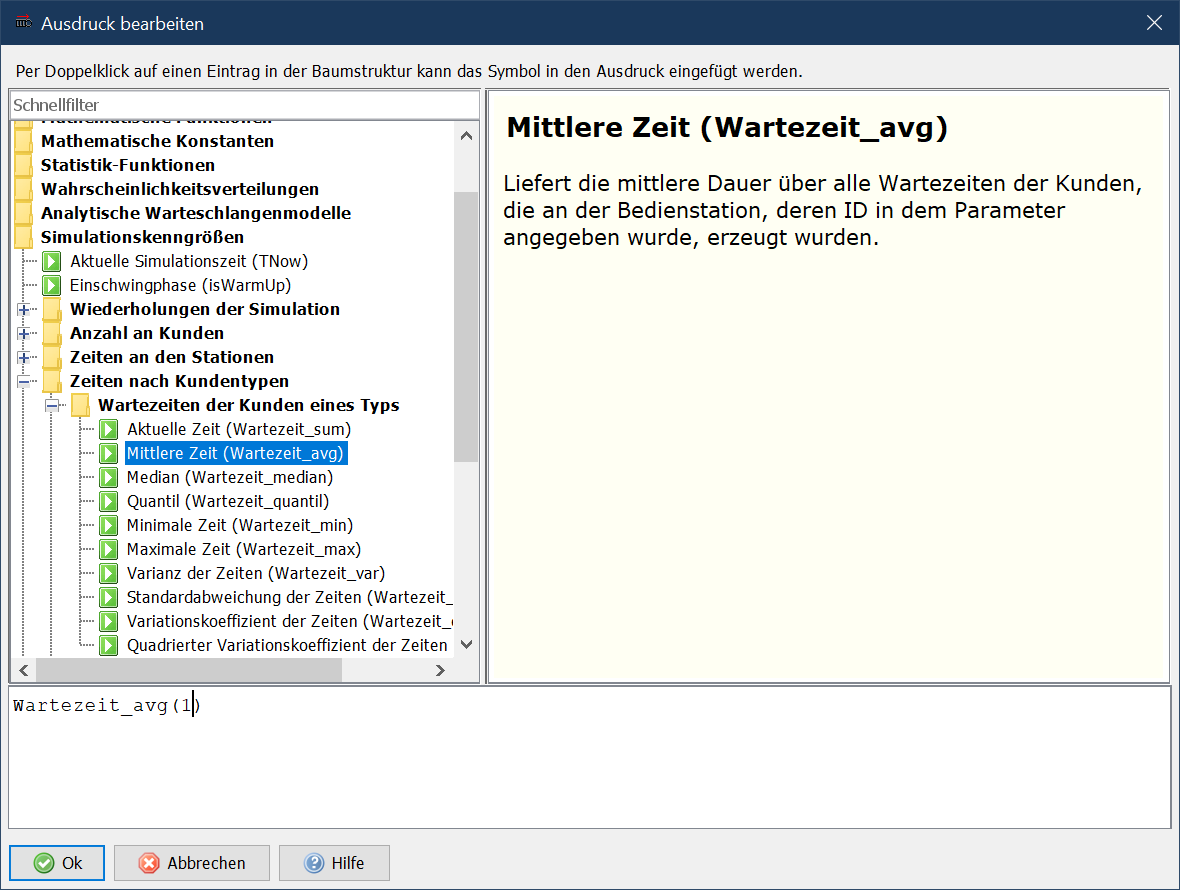
\includegraphics[width=14cm]{DialogExpressionBuilder.png}}
	\label{fig:ExpressionBuilder}
\end{figure}
\part{Referenz der Rechenbefehle}\label{part:Rechenbefehle}

Bei der Verwendung von Rechenbefehlen im Warteschlangensimulator ist zwischen
\textbf{Ausdrücken} und \textbf{Vergleichen} zu unterscheiden. Ausdrücke dienen
dazu, einen Zahlenwert zu berechnen, der dann z.B.\ als Zeitdauer verwendet wird.
Vergleiche liefern eine ja/nein Entscheidung (z.B.\ ob ein Kunde in eine bestimmte
Richtung geleitet werden soll). Im Gegensatz zu Ausdrücken besitzen Vergleiche immer
mindestens einen Vergleichsoperator.

Alle im Folgenden vorgestellten Befehle werden jeweils in jeder beliebigen
\textbf{Groß- und Kleinschreibung} erkannt, d.h.\ es wird nicht zwischen
verschiedenen Groß-/Kleinschreibweisen unterschieden.



\chapter{Konstanten}

Folgende Konstanten stehen in den allen Rechenbefehlen zur Verfügung:

\begin{itemize}

\item
\cmd{e}: Liefert die Basis der Exponentialfunktion $e^x$. Es gilt
$e\approx 2,718281828459$.

\item
\cmd{pi}: Liefert den Wert der Kreiskonstante $\pi$. Es gilt
$\pi\approx 3,1415926535898$.

\end{itemize}



\chapter{Variablen}

Werden Ausdrücke im Kontext eines Kunden berechnet, so stehen die Variablen
\begin{itemize}
\item
\cmd{w} für die \textbf{bisherige Wartezeit} des Kunden,
\item
\cmd{t} für die \textbf{bisherige Transferzeit} des Kunden und
\item
\cmd{p} für die \textbf{bisherige Bedienzeit} des Kunden zur Verfügung.
\end{itemize}

Bei der Berechnung von Score-Werten wird \cmd{w} abweichend nicht mit der bisherigen
gesamten Wartezeit des Kunden belegt, sondern mit der bisherigen Wartezeit an der aktuellen Station.

Des weiteren stehen stets alle Variablen, die über ein Zuweisungselement definiert werden, zur Verfügung.
Vor der ersten Zuweisung eines Wertes an eine Variable hat diese den Wert 0.



\chapter{Grundrechenarten}

Es werden die üblichen Grundrechenarten unterstützt:
\begin{itemize}
\item Addition: \cmd{$+$}
\item Subtraktion: \cmd{$-$}
\item Multiplikation: \cmd{$*$}
\item Division: \cmd{$/$}
\item Potenzieren: \cmd{$\hat~$}
\end{itemize}

Die Regel \textbf{Punkt- vor Strichrechnung} wird dabei berücksichtigt.
Um davon abweichende Auswertungen zu erzwingen, können \textbf{Klammern}
gesetzt werden.



\chapter{Nachgestellte Anweisungen}

Folgende Ausdrücke können unmittelbar hinter eine Zahl geschrieben werden:

\begin{itemize}
\item
\cmd{\%}:
Der Zahlenwert vor diesem Symbol wird als Prozentwert interpretiert,
z.B.\ $30\%=0{,}3$.

\item
\cmd{$^2$}:
Potenziert die Zahl vor diesem Symbol mit 2.

\item
\cmd{$^3$}:
Potenziert die Zahl vor diesem Symbol mit 3.

\item
\cmd{!}:
Berechnet die Fakultät der Zahl vor diesem Ausdruck, z.B.\ $4!=1\cdot2\cdot3\cdot4=24$.

\item
\cmd{$^{\circ}$}:
Rechnet die Zahl vor diesem Symbol von Grad nach Bogenmaß um, z.B.\ $180^{\circ}=3{,}1415\ldots$.\\
(Siehe hierzu auch Abschnitt \ref{sec:Winkelfunktionen} in dem die vom
Warteschlangensimulator unterstützten Winkelfunktionen vorgestellt werden.)
\end{itemize}



\chapter{Allgemeine Funktionen}

\begin{itemize}

\item
\cmd{abs(x)}:
Absolutbetrag, z.B.\ \cm{abs(-5)=5}.

\item
\cmd{binom(n;k)}:
Binomialkoeffizient

\item
\cmd{cbrt(x)}:
Kubikwurzel, z.B.\ \cm{cbrt{27}=3}.

\item
\cmd{ceil(x)}:
Aufrunden, z.B.\ \cm{ceil(2{,}1)=3}

\item
\cmd{exp(x)}:
Exponentialfunktion $e^x$.

\item
\cmd{factorial(x)}:
Fakultät, z.B.\ $4!=1\cdot2\cdot3\cdot4=24$.

\item
\cmd{floor(x)}:
Abrunden, z.B.\ \cm{floor(2{,}9)=2}

\item
\cmd{frac(x)}:
Nachkommaanteil, z.B.\ \cm{frac(1{,}3)=0,3}

\item
\cmd{gamma(x)}:
Gamma-Funktion, z.B.\ \cm{gamma(5)=4!=24}

\item
\cmd{int(x)}:
Ganzzahlanteil, z.B.\ \cm{int(2{,}9)=2}

\item
\cmd{ld(x)}:
Logarithmus zur Basis $2$, z.B.\ \cm{ld(256)=8}.

\item
\cmd{lg(x)}:
Logarithmus zur Basis $10$, z.B.\ \cm{lg(100)=2}.

\item
\cmd{ln(x)}:
Logarithmus zur Basis $e$.

\item
\cmd{log(x)}:
Logarithmus zur Basis $e$.

\item
\cmd{log(x;b)}:
Logarithmus zur Basis $b$.

\item
\cmd{modulo(a;b)} oder \cmd{mod(a;b)}:
Divisionsrest bei Division a/b

\item
\cmd{pow(x;y)}:
Potenzieren $x^y$.

\item
\cmd{random()}:
Liefert eine Zufallszahl zwischen 0 (einschließlich) und 1 (ausschließlich).

\item
\cmd{random(x)}:
Liefert eine Zufallszahl zwischen 0 (einschließlich) und x (ausschließlich).

\item
\cmd{round(x)}:
Runden, z.B.\ \cm{round(4{,}4)=4} und \cm{round(4{,}5)=5}.

\item
\cmd{sign(x)}:
Vorzeichen einer Zahl, z.B.\ \cm{sign(3)=1} und \cm{sign(-3)=-1}.

\item
\cmd{sqr(x)}:
Zahl quadrieren, z.B.\ \cm{sqr(4)=16}.

\item
\cmd{sqrt(x)}:
Quadratwurzel, z.B.\ \cm{sqrt{81}=9}.

\item
\cmd{zeta(x)}:
Zeta-Funktion, z.B.\ \cm{zeta(2)=1{,}64493=$\frac{\pi^2}{6}$}

\end{itemize}



\section{Zufallszahlen}

Mit den folgenden Befehlen können Zufallszahlen, die in einem bestimmten
Bereich \textbf{gleichverteilt} sind erzeugt werden. Im Abschnitt
\ref{sec:Wahrscheinlichkeitsverteilungen} werden weitere Funktionen zur
Erzeugung von Zufallszahlen gemäß bestimmten Verteilungsfunktionen vorgestellt.

\begin{itemize}

\item
\cmd{random()}:
Liefert eine Zufallszahl zwischen 0 (einschließlich) und 1 (ausschließlich).

\item
\cmd{random(x)}:
Liefert eine Zufallszahl zwischen 0 (einschließlich) und x (ausschließlich).

\end{itemize}





\chapter{Winkelfunktionen}\label{sec:Winkelfunktionen}

Die Winkelfunktionen beziehen sich immer auf $2\pi$ als Vollkreis (Bogenmaß, ,,Rad'').
Wenn Winkel in Grad ($360^\circ$ für den Vollkreis) angegeben werden sollen, so müssen
diese bei der Verwendung der elementaren Winkelfunktionen in Bodenmaß umgerechnet werden,
z.B.\ \cm{sin($90^\circ$)=1}.



\section{Elementare Winkelfunktionen}

\begin{itemize}

\item
\cmd{sin(x)}:
Sinus

\item
\cmd{cos(x)}:
Cosinus

\item
\cmd{tan(x)}:
Tangens

\item
\cmd{cot(x)}:
Cotangens

\end{itemize}



\section{Hyperbolische Winkelfunktionen}

\begin{itemize}

\item
\cmd{sinh(x)}:
Sinus hyperbolicus

\item
\cmd{cosh(x)}:
Cosinus hyperbolicus

\item
\cmd{tanh(x)}:
Tangens hyperbolicus

\item
\cmd{coth(x)}:
Cotangens hyperbolicus

\end{itemize}



\section{Umkehrfunktionen der elementaren Winkelfunktionen}

\begin{itemize}

\item
\cmd{arcsin(x)}:
Arcus-Sinus

\item
\cmd{arccos(x)}:
Arcus-Cosinus

\item
\cmd{arctan(x)}:
Arcus-Tangens

\item
\cmd{arccot(x)}:
Arcus-Cotangens

\end{itemize}



\section{Umkehrfunktionen der hyperbolischen Winkelfunktionen}

\begin{itemize}

\item
\cmd{arcsinh(x)}:
Arcus-Sinus hyperbolicus

\item
\cmd{arccosh(x)}:
Arcus-Cosinus hyperbolicus

\item
\cmd{arctanh(x)}:
Arcus-Tangens hyperbolicus

\item
\cmd{arccoth(x)}:
Arcus-Cotangens hyperbolicus

\end{itemize}



\chapter{Funktionen mit mehreren Parametern}

Die folgenden Funktionen können beliebig viele Parameter entgegennehmen.
Die einzelnen Parameter müssen dabei durch Semikolon ,,;'' getrennt
angegeben werden.

\begin{itemize}

\item
\cmd{Min(a;b;c;...)}:
Berechnet das Minimum der übergebenen Zahlen.

\item
\cmd{Max(a;b;c;...)}:
Berechnet das Maximum der übergebenen Zahlen.

\item
\cmd{Sum(a;b;c;...)}:
Berechnet die Summe der übergebenen Zahlen.

\item
\cmd{Mean(a;b;c;...)}:
Berechnet das arithmetische Mittel der übergebenen Zahlen.

\item
\cmd{Median(a;b;c;...)}:
Berechnet den Median der übergebenen Zahlen.

\item
\cmd{Var(a;b;c;...)}:
Berechnet die korrigierte Stichprobenvarianz der übergebenen Zahlen.

\item
\cmd{SD(a;b;c;...)}:
Berechnet die korrigierte Stichprobenstandardabweichung der übergebenen Zahlen.

\item
\cmd{SCV(a;b;c;...)}:
Berechnet den quadrierten Variationskoeffizient der übergebenen Zahlen.

\item
\cmd{CV(a;b;c;...)}:
Berechnet den Variationskoeffizient der übergebenen Zahlen.

\item
\cmd{Sk(a;b;c;...)}:
Berechnet die Schiefe der als Parameter übergebenen Werte.

\item
\cmd{Kurt(a;b;c;...)}:
Berechnet den Exzess (ein Maß für die Wölbung) der als Parameter übergebenen Werte.

\item
\cmd{gcd(a;b;c;...)}:
Berechnet den größten gemeinsamen Teiler (ggT) der übergebenen Zahlen. Die Zahlen werden dabei wenn nötig zu Ganzzahlen gerundet und negative Vorzeichen verworfen.
\item
\cmd{lcm(a;b;c;...)}:
Berechnet das kleinste gemeinsame Vielfache (kgV) der übergebenen Zahlen. Die Zahlen werden dabei wenn nötig zu Ganzzahlen gerundet und negative Vorzeichen verworfen.

\end{itemize}



\chapter{Logik-Funktionen}

\item
\cmd{and(a;b;c;...)}:
Liefert 1, wenn alle Parameter ungleich 0 sind, und 0 sonst.

\item
\cmd{or(a;b;c;...)}:
Liefert 1, wenn mindestens ein Parameter ungleich 0 ist, und 0 sonst.

\item
\cmd{xor(a;b;c;...)}:
Liefert 1, wenn die Anzahl der Parameter mit einem Wert ungleich 0 ungerade ist, und 0 sonst.

\item
\cmd{not(a)}:
Liefert 1, wenn der Parameter 0 ist, und 0 sonst.

\item
\cmd{nand(a;b;c;...)}:
Liefert 0, wenn alle Parameter ungleich 0 sind, und 1 sonst.

\item
\cmd{nor(a;b;c;...)}:
Liefert 0, wenn mindestens ein Parameter ungleich 0 ist, und 1 sonst.

\item
\cmd{nxor(a;b;c;...)}:
Liefert 1, wenn die Anzahl der Parameter mit einem Wert ungleich 0 gerade ist, und 0 sonst.



\chapter{Wahrscheinlichkeitsverteilungen}\label{sec:Wahrscheinlichkeitsverteilungen}

Mit Hilfe der folgenden Befehle können sowohl Werte der Dichte und der Verteilungsfunktion
der folgenden Wahrscheinlichkeitsverteilungen berechnet werden als auch Zufallszahlen
auf Basis einer dieser Wahrscheinlichkeitsverteilungen berechnet werden:


\section{Hypergeometrische Verteilung \texorpdfstring{$Hg(N,K,n)$}{Hg(N,K,n)}}

\begin{itemize}

\item
\cmd{HypergeometricDist(k;N;K;n)}:
Berechnet die Zähldichte an der Stelle $k$.

\item
\cmd{HypergeometricDist(N;K;n)}:
Erzeugt eine Zufallszahl gemäß der Verteilung.

\end{itemize}



\section{Binomial-Verteilung \texorpdfstring{$B(n,p)$}{B(n,p)}}

\begin{itemize}

\item
\cmd{BinomialDist(k;n;p)}:
Berechnet die Zähldichte an der Stelle $k$.


\item
\cmd{BinomialDist(n;p)}:
Erzeugt eine Zufallszahl gemäß der Verteilung.

\end{itemize}



\section{Binomial-Verteilung mit Mittelwert \texorpdfstring{$a$}{a} und Standardabweichung \texorpdfstring{$b$}{b}}

\begin{itemize}

\item
\cmd{BinomialDistDirect(k;a;b)}:
Berechnet die Zähldichte an der Stelle $k$.


\item
\cmd{BinomialDistDirect(a;b)}:
Erzeugt eine Zufallszahl gemäß der Verteilung.

\end{itemize}



\section{Poisson-Verteilung \texorpdfstring{$P(l)$}{P(l)}}

\begin{itemize}

\item
\cmd{PoissonDist(k;l)}:
Berechnet die Zähldichte an der Stelle $k$.

\item
\cmd{PoissonDist(l)}:
Erzeugt eine Zufallszahl gemäß der Verteilung.

\end{itemize}



\section{Zeta-Verteilung \texorpdfstring{$Z(s)$}{Z(s)}}

\begin{itemize}

\item
\cmd{ZetaDist(k;s)}:
Berechnet die Zähldichte an der Stelle $k$.

\item
\cmd{ZetaDist(s)}:
Erzeugt eine Zufallszahl gemäß der Verteilung.

\end{itemize}



\section{Negative Binomial-Verteilung \texorpdfstring{$NB(r,p)$}{NB(r,p)}}

\begin{itemize}

\item
\cmd{NegativeBinomialDist(k;r;p)}:
Berechnet die Zähldichte an der Stelle $k$.


\item
\cmd{NegativeBinomialDist(r;p)}:
Erzeugt eine Zufallszahl gemäß der Verteilung.

\end{itemize}



\section{Negative Binomial-Verteilung mit Mittelwert \texorpdfstring{$a$}{a} und Standardabweichung \texorpdfstring{$b$}{b}}

\begin{itemize}

\item
\cmd{NegativeBinomialDistDirect(k;a;b)}:
Berechnet die Zähldichte an der Stelle $k$.


\item
\cmd{NegativeBinomialDistDirect(a;b)}:
Erzeugt eine Zufallszahl gemäß der Verteilung.

\end{itemize}



\section{Diskrete Gleichverteilung über das Intervall \texorpdfstring{$[a;b]$}{[a;b]} (Ganzzahlen)}

\begin{itemize}

\item
\cmd{DiscreteUniformDist(k;a;b)}:
Berechnet die Zähldichte an der Stelle $k$.

\item
\cmd{DiscreteUniformDist(a;b)}:
Erzeugt eine Zufallszahl gemäß der Verteilung.

\end{itemize}



\section{Exponentialverteilung mit Mittelwert \texorpdfstring{$a$}{a}}

\begin{itemize}

\item
\cmd{ExpDist(x;a;0)}:
Berechnet die Dichte an der Stelle $x$.

\item
\cmd{ExpDist(x;a;1)}:
Berechnet den Wert der Verteilungsfunktion an der Stelle $x$.

\item
\cmd{ExpDist(a)}:
Erzeugt eine Zufallszahl gemäß der Verteilung.

\item
\cmd{ExpDistRange(min;max;a)}:
Erzeugt eine Zufallszahl gemäß der Verteilung und stellt dabei sicher, dass sich das Ergebnis in dem Bereich von $min$ bis $max$ befindet.

\end{itemize}



\section{Gleichverteilung über das Intervall \texorpdfstring{$[a;b]$}{[a;b]}}

\begin{itemize}

\item
\cmd{UniformDist(x;a;b;0)}:
Berechnet die Dichte an der Stelle $x$.

\item
\cmd{UniformDist(x;a;b;1)}:
Berechnet den Wert der Verteilungsfunktion an der Stelle $x$.

\item
\cmd{UniformDist(a;b)}:
Erzeugt eine Zufallszahl gemäß der Verteilung.

\end{itemize}



\section{Normalverteilung mit Mittelwert \texorpdfstring{$a$}{a} und Standardabweichung \texorpdfstring{$b$}{b}}

\begin{itemize}

\item
\cmd{NormalDist(x;a;b;0)}:
Berechnet die Dichte an der Stelle $x$.

\item
\cmd{NormalDist(x;a;b;1)}:
Berechnet den Wert der Verteilungsfunktion an der Stelle $x$.

\item
\cmd{NormalDist(a;b)}:
Erzeugt eine Zufallszahl gemäß der Verteilung.

\item
\cmd{NormalDistRange(min;max;a;b)}:
Erzeugt eine Zufallszahl gemäß der Verteilung und stellt dabei sicher, dass sich das Ergebnis in dem Bereich von $min$ bis $max$ befindet.

\end{itemize}



\section{Lognormalverteilung mit Mittelwert \texorpdfstring{$a$}{a} und Standardabweichung \texorpdfstring{$b$}{b}}

\begin{itemize}

\item
\cmd{LogNormalDist(x;a;b;0)}:
Berechnet die Dichte an der Stelle $x$.

\item
\cmd{LogNormalDist(x;a;b;1)}:
Berechnet den Wert der Verteilungsfunktion an der Stelle $x$.

\item
\cmd{LogNormalDist(a;b)}:
Erzeugt eine Zufallszahl gemäß der Verteilung.

\item
\cmd{LogNormalDistRange(min;max;a;b)}:
Erzeugt eine Zufallszahl gemäß der Verteilung und stellt dabei sicher, dass sich das Ergebnis in dem Bereich von $min$ bis $max$ befindet.

\end{itemize}



\section{Gamma-Verteilung mit Parametern \texorpdfstring{$\alpha=a$}{a} und \texorpdfstring{$\beta=b$}{b}}

\begin{itemize}

\item
\cmd{GammaDist(x;a;b;0)}:
Berechnet die Dichte an der Stelle $x$.

\item
\cmd{GammaDist(x;a;b;1)}:
Berechnet den Wert der Verteilungsfunktion an der Stelle $x$.

\item
\cmd{GammaDist(a;b)}:
Erzeugt eine Zufallszahl gemäß der Verteilung.

\item
\cmd{GammaDistRange(min;max;a;b)}:
Erzeugt eine Zufallszahl gemäß der Verteilung und stellt dabei sicher, dass sich das Ergebnis in dem Bereich von $min$ bis $max$ befindet.

\end{itemize}



\section{Gamma-Verteilung mit Mittelwert \texorpdfstring{$a$}{a} und Standardabweichung \texorpdfstring{$b$}{b}}

\begin{itemize}

\item
\cmd{GammaDistDirect(x;a;b;0)}:
Berechnet die Dichte an der Stelle $x$.

\item
\cmd{GammaDistDirect(x;a;b;1)}:
Berechnet den Wert der Verteilungsfunktion an der Stelle $x$.

\item
\cmd{GammaDistDirect(a;b)}:
Erzeugt eine Zufallszahl gemäß der Verteilung.

\item
\cmd{GammaDistDirectRange(min;max;a;b)}:
Erzeugt eine Zufallszahl gemäß der Verteilung und stellt dabei sicher, dass sich das Ergebnis in dem Bereich von $min$ bis $max$ befindet.

\end{itemize}



\section{Erlang-Verteilung mit Parametern \texorpdfstring{$n$}{n} und \texorpdfstring{$\lambda=l$}{l}}

\begin{itemize}

\item
\cmd{ErlangDist(x;n;l;0)}:
Berechnet die Dichte an der Stelle $x$.

\item
\cmd{ErlangDist(x;n;l;1)}:
Berechnet den Wert der Verteilungsfunktion an der Stelle $x$.

\item
\cmd{ErlangDist(n;b)}:
Erzeugt eine Zufallszahl gemäß der Verteilung.

\item
\cmd{ErlangDistRange(min;max;n;b)}:
Erzeugt eine Zufallszahl gemäß der Verteilung und stellt dabei sicher, dass sich das Ergebnis in dem Bereich von $min$ bis $max$ befindet.

\end{itemize}



\section{Beta-Verteilung in dem Intervall \texorpdfstring{$[a;b]$}{[a;b]} und mit Parametern \texorpdfstring{$\alpha=c$}{c} und \texorpdfstring{$\beta=d$}{d}}

\begin{itemize}

\item
\cmd{BetaDist(x;a;b;c;d;0)}:
Berechnet die Dichte an der Stelle $x$.

\item
\cmd{BetaDist(x;a;b;c;d;1)}:
Berechnet den Wert der Verteilungsfunktion an der Stelle $x$.

\item
\cmd{BetaDist(a;b;c;d)}:
Erzeugt eine Zufallszahl gemäß der Verteilung.

\end{itemize}



\section{Beta-Verteilung in dem Intervall \texorpdfstring{$[a;b]$}{[a;b]} und mit Mittelwert \texorpdfstring{$c$}{c} und Standardabweichung \texorpdfstring{$d$}{d}}

\begin{itemize}

\item
\cmd{BetaDistDirect(x;a;b;c;d;0)}:
Berechnet die Dichte an der Stelle $x$.

\item
\cmd{BetaDistDirect(x;a;b;c;d;1)}:
Berechnet den Wert der Verteilungsfunktion an der Stelle $x$.

\item
\cmd{BetaDistDirect(a;b;c;d)}:
Erzeugt eine Zufallszahl gemäß der Verteilung.

\end{itemize}



\section{Weibull-Verteilung mit Parametern Scale=\texorpdfstring{$a$}{a} und Form=\texorpdfstring{$b$}{b}}

\begin{itemize}

\item
\cmd{WeibullDist(x;a;b;0)}:
Berechnet die Dichte an der Stelle $x$.

\item
\cmd{WeibullDist(x;a;b;1)}:
Berechnet den Wert der Verteilungsfunktion an der Stelle $x$.

\item
\cmd{WeibullDist(a;b)}:
Erzeugt eine Zufallszahl gemäß der Verteilung.

\item
\cmd{WeibullDistRange(min;max;a;b)}:
Erzeugt eine Zufallszahl gemäß der Verteilung und stellt dabei sicher, dass sich das Ergebnis in dem Bereich von $min$ bis $max$ befindet.

\end{itemize}



\section{Cauchy-Verteilung mit Mittelwert \texorpdfstring{$a$}{a} und Scale=\texorpdfstring{$b$}{b}}

\begin{itemize}

\item
\cmd{CauchyDist(x;a;b;0)}:
Berechnet die Dichte an der Stelle $x$.

\item
\cmd{CauchyDist(x;a;b;1)}:
Berechnet den Wert der Verteilungsfunktion an der Stelle $x$.

\item
\cmd{CauchyDist(a;b)}:
Erzeugt eine Zufallszahl gemäß der Verteilung.

\item
\cmd{CauchyDistRange(min;max;a;b)}:
Erzeugt eine Zufallszahl gemäß der Verteilung und stellt dabei sicher, dass sich das Ergebnis in dem Bereich von $min$ bis $max$ befindet.

\end{itemize}



\section{\texorpdfstring{Chi$^2$}{Chi2}-Verteilung mit \texorpdfstring{$n$}{n} Freiheitsgraden}

\begin{itemize}

\item
\cmd{ChiSquareDist(x;n;0)}:
Berechnet die Dichte an der Stelle $x$.

\item
\cmd{ChiSquareDist(x;n;1)}:
Chi$^2$-Verteilung mit $n$ Freiheitsgraden.

\item
\cmd{ChiSquareDist(n)}:
Erzeugt eine Zufallszahl gemäß der Verteilung.

\item
\cmd{ChiSquareDistRange(min;max;n)}:
Erzeugt eine Zufallszahl gemäß der Verteilung und stellt dabei sicher, dass sich das Ergebnis in dem Bereich von $min$ bis $max$ befindet.

\end{itemize}



\section{Chi-Verteilung mit \texorpdfstring{$n$}{n} Freiheitsgraden}

\begin{itemize}

\item
\cmd{ChiDist(x;n;0)}:
Berechnet die Dichte an der Stelle $x$.

\item
\cmd{ChiDist(x;n;1)}:
Chi-Verteilung mit $n$ Freiheitsgraden.

\item
\cmd{ChiDist(n)}:
Erzeugt eine Zufallszahl gemäß der Verteilung.

\item
\cmd{ChiDistRange(min;max;n)}:
Erzeugt eine Zufallszahl gemäß der Verteilung und stellt dabei sicher, dass sich das Ergebnis in dem Bereich von $min$ bis $max$ befindet.

\end{itemize}



\section{F-Verteilung mit \texorpdfstring{$a$}{a} Freiheitsgraden im Zähler und \texorpdfstring{$b$}{b} Freiheitsgraden im Nenner}

\begin{itemize}

\item
\cmd{FDist(x;a;b;0)}:
Berechnet die Dichte an der Stelle $x$.

\item
\cmd{FDist(x;a;b;1)}:
Berechnet den Wert der Verteilungsfunktion an der Stelle $x$.

\item
\cmd{FDist(a;b)}:
Erzeugt eine Zufallszahl gemäß der Verteilung.

\item
\cmd{FDistRange(min;max;a;b)}:
Erzeugt eine Zufallszahl gemäß der Verteilung und stellt dabei sicher, dass sich das Ergebnis in dem Bereich von $min$ bis $max$ befindet.

\end{itemize}



\section{Johnson-SU-Verteilung mit den Parametern \texorpdfstring{$\gamma=a$}{a}, \texorpdfstring{$\xi=b$}{b}, \texorpdfstring{$\delta=c$}{c} und \texorpdfstring{$\lambda=d$}{d}}

\begin{itemize}

\item
\cmd{JohnsonSUDist(x;a;b;c;d;0)}:
Berechnet die Dichte an der Stelle $x$.

\item
\cmd{JohnsonSUDist(x;a;b;c;d;1)}:
Berechnet den Wert der Verteilungsfunktion an der Stelle $x$.

\item
\cmd{JohnsonSUDist(a;b;c;d)}:
Erzeugt eine Zufallszahl gemäß der Verteilung.  

\item
\cmd{JohnsonSUDistRange(min;max;a;b;c;d)}:
Erzeugt eine Zufallszahl gemäß der Verteilung und stellt dabei sicher, dass sich das Ergebnis in dem Bereich von $min$ bis $max$ befindet.

\end{itemize}



\section{Dreiecksverteilung über \texorpdfstring{$[a;c]$}{[a;c]} mit der höchsten Wahrscheinlichkeitsdichte bei \texorpdfstring{$b$}{b}}

\begin{itemize}

\item
\cmd{TriangularDist(x;a;b;c;0)}:
Berechnet die Dichte an der Stelle $x$.

\item
\cmd{TriangularDist(x;a;b;c;1)}:
Berechnet den Wert der Verteilungsfunktion an der Stelle $x$.

\item
\cmd{TriangularDist(a;b;c)}:
Erzeugt eine Zufallszahl gemäß der Verteilung.

\end{itemize}



\section{Pert-Verteilung über \texorpdfstring{$[a;c]$}{[a;c]} mit der höchsten Wahrscheinlichkeitsdichte bei \texorpdfstring{$b$}{b}}

\begin{itemize}

\item
\cmd{PertDist(x;a;b;c;0)}:
Berechnet die Dichte an der Stelle $x$.

\item
\cmd{PertDist(x;a;b;c;1)}:
Berechnet den Wert der Verteilungsfunktion an der Stelle $x$.

\item
\cmd{PertDist(a;b;c)}:
Erzeugt eine Zufallszahl gemäß der Verteilung.

\end{itemize}



\section{Laplace-Verteilung mit Mittelwert \texorpdfstring{$mu$}{mu} und Skalierungsfaktor \texorpdfstring{$b$}{b}}

\begin{itemize}

\item
\cmd{LaplaceDist(x;mu;b;0)}:
Berechnet die Dichte an der Stelle $x$.

\item
\cmd{LaplaceDist(x;mu;b;1)}:
Berechnet den Wert der Verteilungsfunktion an der Stelle $x$.

\item
\cmd{LaplaceDist(mu;b)}:
Erzeugt eine Zufallszahl gemäß der Verteilung.

\item
\cmd{LaplaceDistRange(min;max;mu;b)}:
Erzeugt eine Zufallszahl gemäß der Verteilung und stellt dabei sicher, dass sich das Ergebnis in dem Bereich von $min$ bis $max$ befindet.

\end{itemize}



\section{Pareto-Verteilung mit Skalierungsparameter \texorpdfstring{$x_{\rm min}=xmin$}{xmin} und Formparameter \texorpdfstring{$\alpha=a$}{a}}

\begin{itemize}

\item
\cmd{ParetoDist(x;xmin;a;0)}:
Berechnet die Dichte an der Stelle $x$.

\item
\cmd{ParetoDist(x;xmin;a;1)}:
Berechnet den Wert der Verteilungsfunktion an der Stelle $x$.

\item
\cmd{ParetoDist(xmin;a)}:
Erzeugt eine Zufallszahl gemäß der Verteilung.

\end{itemize}



\section{Logistische Verteilung mit Mittelwert \texorpdfstring{$\mu=mu$}{mu} und Skalierungsparameter \texorpdfstring{$s$}{s}}

\begin{itemize}

\item
\cmd{LogisticDist(x;mu;s;0)}:
Berechnet die Dichte an der Stelle $x$.

\item
\cmd{LogisticDist(x;mu;s;1)}:
Berechnet den Wert der Verteilungsfunktion an der Stelle $x$.

\item
\cmd{LogisticDist(mu;s)}:
Erzeugt eine Zufallszahl gemäß der Verteilung.

\item
\cmd{LogisticDistRange(min;max;mu;s)}:
Erzeugt eine Zufallszahl gemäß der Verteilung und stellt dabei sicher, dass sich das Ergebnis in dem Bereich von $min$ bis $max$ befindet.

\end{itemize}


	
\section{Inverse Gauß-Verteilung mit \texorpdfstring{$\lambda=l$}{l} und Mittelwert \texorpdfstring{$mu$}{mu}}

\begin{itemize}

\item
\cmd{InverseGaussianDist(x;l;mu;0)}:
Berechnet die Dichte an der Stelle $x$.

\item
\cmd{InverseGaussianDist(x;l;mu;1)}:
Berechnet den Wert der Verteilungsfunktion an der Stelle $x$.

\item
\cmd{InverseGaussianDist(l;mu)}:
Erzeugt eine Zufallszahl gemäß der Verteilung.

\item
\cmd{InverseGaussianDistRange(min;max;l;mu)}:
Erzeugt eine Zufallszahl gemäß der Verteilung und stellt dabei sicher, dass sich das Ergebnis in dem Bereich von $min$ bis $max$ befindet.

\end{itemize}



\section{Rayleigh-Verteilung mit Mittelwert \texorpdfstring{$mu$}{mu}}

\begin{itemize}

\item
\cmd{RayleighDist(x;mu;0)}:
Berechnet die Dichte an der Stelle $x$.

\item
\cmd{RayleighDist(x;mu;1)}:
Berechnet den Wert der Verteilungsfunktion an der Stelle $x$.

\item
\cmd{RayleighDist(mu)}:
Erzeugt eine Zufallszahl gemäß der Verteilung.

\item
\cmd{RayleighDistRange(min;max;mu)}:
Erzeugt eine Zufallszahl gemäß der Verteilung und stellt dabei sicher, dass sich das Ergebnis in dem Bereich von $min$ bis $max$ befindet.

\end{itemize}



\section{Log-Logistische Verteilung mit \texorpdfstring{$\alpha$}{alpha} und Mittelwert \texorpdfstring{$\beta$}{beta}}

\begin{itemize}

\item
\cmd{LogLogisticDist(x;alpha;beta;0)}:
Berechnet die Dichte an der Stelle $x$.

\item
\cmd{LogLogisticDist(x;alpha;beta;1)}:
Berechnet den Wert der Verteilungsfunktion an der Stelle $x$.

\item
\cmd{LogLogisticDist(alpha;beta)}:
Erzeugt eine Zufallszahl gemäß der Verteilung.

\item
\cmd{LogLogisticDistRange(min;max;alpha;beta)}:
Erzeugt eine Zufallszahl gemäß der Verteilung und stellt dabei sicher, dass sich das Ergebnis in dem Bereich von $min$ bis $max$ befindet.

\end{itemize}



\section{Potenzverteilung auf dem Bereich \texorpdfstring{$[a;b]$}{[a;b]} mit Exponent \texorpdfstring{$c$}{c}}

\begin{itemize}

\item
\cmd{PowerDist(x;a;b;c;0)}:
Berechnet die Dichte an der Stelle $x$.

\item
\cmd{PowerDist(x;a;b;c;1)}:
Berechnet den Wert der Verteilungsfunktion an der Stelle $x$.

\item
\cmd{PowerDist(a;b;c)}:
Erzeugt eine Zufallszahl gemäß der Verteilung.

\end{itemize}



\section{Gumbel-Verteilung mit Erwartungswert \texorpdfstring{$a$}{a} und Standardabweichung \texorpdfstring{$b$}{b}}

\begin{itemize}

\item
\cmd{GumbelDist(x;a;b;0)}:
Berechnet die Dichte an der Stelle $x$.

\item
\cmd{GumbelDist(x;a;b;1)}:
Berechnet den Wert der Verteilungsfunktion an der Stelle $x$.

\item
\cmd{GumbelDist(a;b)}:
Erzeugt eine Zufallszahl gemäß der Verteilung.

\item
\cmd{GumbelDistRange(min;max;a;b)}:
Erzeugt eine Zufallszahl gemäß der Verteilung und stellt dabei sicher, dass sich das Ergebnis in dem Bereich von $min$ bis $max$ befindet.

\end{itemize}



\section{Fatigue-Life-Verteilung mit Lageparameter \texorpdfstring{$\mu$}{mu}, Skalierungsparameter \texorpdfstring{$\beta$}{beta} und Formparameter \texorpdfstring{$\gamma$}{gamma}}

\begin{itemize}

\item
\cmd{FatigueLifeDist(x;mu;beta;gamma;0)}:
Berechnet die Dichte an der Stelle $x$.

\item
\cmd{FatigueLifeDist(x;mu;beta;gamma;1)}:
Berechnet den Wert der Verteilungsfunktion an der Stelle $x$.

\item
\cmd{FatigueLifeDist(mu;beta;gamma)}:
Erzeugt eine Zufallszahl gemäß der Verteilung.

\item
\cmd{FatigueLifeDistRange(min;max;mu;beta;gamma)}:
Erzeugt eine Zufallszahl gemäß der Verteilung und stellt dabei sicher, dass sich das Ergebnis in dem Bereich von $min$ bis $max$ befindet.

\end{itemize}



\section{Frechet-Verteilung mit Lageparameter \texorpdfstring{$\delta$}{delta}, Skalierungsparameter \texorpdfstring{$\beta$}{beta} und Formparameter \texorpdfstring{$\alpha$}{alpha}}

\begin{itemize}

\item
\cmd{FrechetDist(x;delta;beta;alpha;0)}:
Berechnet die Dichte an der Stelle $x$.

\item
\cmd{FrechetDist(x;delta;beta;alpha;1)}:
Berechnet den Wert der Verteilungsfunktion an der Stelle $x$.

\item
\cmd{FrechetDist(delta;beta;alpha)}:
Erzeugt eine Zufallszahl gemäß der Verteilung.

\item
\cmd{FrechetDistRange(min;max;delta;beta;alpha)}:
Erzeugt eine Zufallszahl gemäß der Verteilung und stellt dabei sicher, dass sich das Ergebnis in dem Bereich von $min$ bis $max$ befindet.

\end{itemize}



\section{Hyperbolische Sekanten-Verteilung mit Mittelwert \texorpdfstring{$a$}{a} und Standardabweichung \texorpdfstring{$b$}{b}}

\begin{itemize}

\item
\cmd{HyperbolicSecantDist(x;a;b;0)}:
Berechnet die Dichte an der Stelle $x$.

\item
\cmd{HyperbolicSecantDist(x;a;b;1)}:
Berechnet den Wert der Verteilungsfunktion an der Stelle $x$.

\item
\cmd{HyperbolicSecantDist(a;b)}:
Erzeugt eine Zufallszahl gemäß der Verteilung.

\item
\cmd{HyperbolicSecantDistRange(min;max;a;b)}:
Erzeugt eine Zufallszahl gemäß der Verteilung und stellt dabei sicher, dass sich das Ergebnis in dem Bereich von $min$ bis $max$ befindet.

\end{itemize}



\section{Linke Sägezahnverteilung über \texorpdfstring{$[a;b]$}{[a;b]}}

\begin{itemize}

\item
\cmd{LeftSawtoothDist(x;a;b;0)}:
Berechnet die Dichte an der Stelle $x$.

\item
\cmd{LeftSawtoothDist(x;a;b;1)}:
Berechnet den Wert der Verteilungsfunktion an der Stelle $x$.

\item
\cmd{LeftSawtoothDist(a;b)}:
Erzeugt eine Zufallszahl gemäß der Verteilung.

\end{itemize}



\section{Linke Sägezahnverteilung über mit Erwartungswert \texorpdfstring{$a$}{a} und Standardabweichung \texorpdfstring{$b$}{b}}

\begin{itemize}

\item
\cmd{LeftSawtoothDistDirect(x;a;b;0)}:
Berechnet die Dichte an der Stelle $x$.

\item
\cmd{LeftSawtoothDistDirect(x;a;b;1)}:
Berechnet den Wert der Verteilungsfunktion an der Stelle $x$.

\item
\cmd{LeftSawtoothDistDirect(a;b)}:
Erzeugt eine Zufallszahl gemäß der Verteilung.

\end{itemize}



\section{Rechte Sägezahnverteilung über \texorpdfstring{$[a;b]$}{[a;b]}}

\begin{itemize}

\item
\cmd{RightSawtoothDist(x;a;b;0)}:
Berechnet die Dichte an der Stelle $x$.

\item
\cmd{RightSawtoothDist(x;a;b;1)}:
Berechnet den Wert der Verteilungsfunktion an der Stelle $x$.

\item
\cmd{RightSawtoothDist(a;b)}:
Erzeugt eine Zufallszahl gemäß der Verteilung.

\end{itemize}



\section{Rechte Sägezahnverteilung über mit Erwartungswert \texorpdfstring{$a$}{a} und Standardabweichung \texorpdfstring{$b$}{b}}

\begin{itemize}

\item
\cmd{RightSawtoothDistDirect(x;a;b;0)}:
Berechnet die Dichte an der Stelle $x$.

\item
\cmd{RightSawtoothDistDirect(x;a;b;1)}:
Berechnet den Wert der Verteilungsfunktion an der Stelle $x$.

\item
\cmd{RightSawtoothDistDirect(a;b)}:
Erzeugt eine Zufallszahl gemäß der Verteilung.

\end{itemize}



\section{Levy-Verteilung mit Lageparameter \texorpdfstring{$\mu$}{mu} und Formparameter \texorpdfstring{$c$}{c}}

\begin{itemize}

\item
\cmd{LevyDist(x;mu;c;0)}:
Berechnet die Dichte an der Stelle $x$.

\item
\cmd{LevyDist(x;mu;c;1)}:
Berechnet den Wert der Verteilungsfunktion an der Stelle $x$.

\item
\cmd{LevyDist(mu;c)}:
Erzeugt eine Zufallszahl gemäß der Verteilung.

\end{itemize}



\section{Maxwell-Boltzmann-Verteilung mit Parameter a}

\begin{itemize}

\item
\cmd{MaxwellBoltzmannDist(x;a;0)}:
Berechnet die Dichte an der Stelle $x$.

\item
\cmd{MaxwellBoltzmannDist(x;a;1)}:
Berechnet den Wert der Verteilungsfunktion an der Stelle $x$.

\item
\cmd{MaxwellBoltzmannDist(a)}:
Erzeugt eine Zufallszahl gemäß der Verteilung.

\end{itemize}



\section{Verteilung aus empirischen Daten}

\begin{itemize}

\item
\cmd{EmpirischeDichte(x;wert1;wert2;wert3;...;max)}:\\
Berechnet die Dichte an der Stelle $x$.
Die angegebenen Werte werden dabei auf den Bereich von 0 bis $max$ verteilt.

\item
\cmd{EmpirischeVerteilung(x;wert1;wert2;wert3;...;max)}:\\
Berechnet den Wert der Verteilungsfunktion an der Stelle $x$.
Die angegebenen Werte werden dabei auf den Bereich von 0 bis $max$ verteilt.

\item
\cmd{EmpirischeZufallszahl(wert1;wert2;wert3;...;max)}:\\
Erzeugt eine Zufallszahl gemäß der Verteilung.
Die angegebenen Werte werden dabei auf den Bereich von 0 bis $max$ verteilt.

\item
\cmd{EmpirischeVerteilungMittelwert(wert1;wert2;wert3;...;max)}:\\
Liefert den Erwartungswert der Verteilung.

\item
\cmd{EmpirischeVerteilungMedian(wert1;wert2;wert3;...;max)}:\\
Liefert den Median der Verteilung.

\item
\cmd{EmpirischeVerteilungQuantil(wert1;wert2;wert3;...;max;p)}:\\
Liefert das Quantil zur Wahrscheinlichkeit p der Verteilung.

\item
\cmd{EmpirischeVerteilungSD(wert1;wert2;wert3;...;max)}:\\
Liefert die Standardabweichung der Verteilung.

\item
\cmd{EmpirischeVerteilungVar(wert1;wert2;wert3;...;max)}:\\
Liefert die Varianz der Verteilung.

\item
\cmd{EmpirischeVerteilungCV(wert1;wert2;wert3;...;max)}:\\
Liefert den Variationskoeffizient der Verteilung.

\end{itemize}



\section{Zufällige Auswahl eines von mehreren Werten}

\cmd{RandomValues(rate1;wert1;rate2;wert2;...)}\\
Wählt jeweils zufällig (gemäß den angegebenen Raten) einen der angegebenen Werte aus.

Beispiel:
\cmd{RandomValues(1;3;2;5)}\\
liefert in $\frac{1}{3}$ (Rate 1) der Fälle den Wert 3 und in $\frac{2}{3}$ (Rate 2) der Fälle den Wert 5.



\section{Zufallszahlen gemäß benutzerdefinierter Verteilung}

\cmd{RandomGenerator(distribution(RandomGeneratorX());min;max)}\\
Erzeugt eine Zufallszahl gemäß der im ersten Parameter angegebenen Verteilungsfunktion (in der über \cm{RandomGeneratorX()} der Parameter spezifiziert wird) im Bereich, der über die Parameter zwei und drei festgelegt wird.

Beispiel:\\
\cmd{RandomGenerator(ExpDist(RandomGeneratorX();5;1);0;100)}\\
erzeugt eine Zufallszahl gemäß der Exponentialverteilung mit Erwartungswert 5.



\chapter{Erlang-C-Rechner}

Mit Hilfe des folgenden Befehls können verschiedene Kenngrößen auf Basis der
erweiterten Erlang-C-Formel berechnet werden:

\begin{itemize}

\item
\cmd{ErlangC(lambda;mu;nu;c;K;-1)}:\\
Berechnet die mittlere Warteschlangenlänge $\E[N_Q]$. 

\item
\cmd{ErlangC(lambda;mu;nu;c;K;-2)}:\\
Berechnet die mittlere Anzahl an Kunden im System $\E[N]$.

\item
\cmd{ErlangC(lambda;mu;nu;c;K;-3)}:\\
Berechnet die mittlere Wartezeit $\E[W]$.

\item
\cmd{ErlangC(lambda;mu;nu;c;K;-4)}:\\
Berechnet die mittlere Verweilzeit $\E[V]$.

\item
\cmd{ErlangC(lambda;mu;nu;c;K;-5)}:\\
Berechnet die mittlere Erreichbarkeit $1-P(A)$.

\item
\cmd{ErlangC(lambda;mu;nu;c;K;t)}:\\
Berechnet die Wahrscheinlichkeit für den Service-Level an der $t$-Sekunden-Schranke $P(W\le t)$.

\end{itemize}

Die Parameter haben dabei folgende Bedeutungen:
\begin{itemize}
\item
\cm{lambda}:\\
Ankunftsrate $\lambda$ (in Kunden pro Zeiteinheit), d.h.\ Kehrwert der mittleren Zwischenankunftszeit.
\item
\cm{mu}:\\
Bedienrate $\mu$ (in Kunden pro Zeiteinheit), d.h.\ Kehrwert der mittleren Bediendauer.
\item
\cm{nu}:\\
Abbruchrate $\nu$ (in Kunden pro Zeiteinheit), d.h.\ Kehrwert der mittleren Wartezeittoleranz.
\item
\cm{c}:\\
Anzahl an verfügbaren parallel arbeitenden Bedienern.
\item
\cm{K}:\\
Anzahl an verfügbaren Plätzen im System (Warte- und Bedienplätze zusammen, d.h.\ es gilt $K\ge c$).
\end{itemize}



\chapter{Allen-Cunneen-Approximationsformel}

Mit Hilfe des folgenden Befehls können verschiedene Kenngrößen auf Basis der
Allen-Cunneen-Approxi\-ma\-ti\-ons\-for\-mel berechnet werden:

\begin{itemize}

\item
\cmd{AllenCunneen(lambda;mu;cvI;cvS;c;-1)}:\\
Berechnet die mittlere Warteschlangenlänge $E[N_Q]$. 

\item
\cmd{AllenCunneen(lambda;mu;cvI;cvS;c;-2)}:\\
Berechnet die mittlere Anzahl an Kunden im System $\E[N]$.

\item
\cmd{AllenCunneen(lambda;mu;cvI;cvS;c;-3)}:\\
Berechnet die mittlere Wartezeit $\E[W]$.

\item
\cmd{AllenCunneen(lambda;mu;cvI;cvS;c;-4)}:\\
Berechnet die mittlere Verweilzeit $\E[V]$.
\end{itemize}

Die Parameter haben dabei folgende Bedeutungen:
\begin{itemize}
\item
\cm{lambda}:\\
Ankunftsrate $\lambda$ (in Kunden pro Zeiteinheit), d.h.\ Kehrwert der mittleren Zwischenankunftszeit.
\item
\cm{mu}:\\
Bedienrate $\mu$ (in Kunden pro Zeiteinheit), d.h.\ Kehrwert der mittleren Bediendauer.
\item
\cm{cvI}:\\
Variationskoeffizient der Zwischenankunftszeiten $\CV[I]$ (kleine Werte bedeuten, dass die Ankünfte sehr gleichmäßig erfolgen).
\item
\cm{cvS}:\\
Variationskoeffizient der Bedienzeiten $\CV[S]$ (kleine Werte bedeuten, dass die Bedienung sehr gleichmäßig erfolgen).
\item
\cm{c}:\\
Anzahl an verfügbaren parallel arbeitenden Bedienern.
\end{itemize}
\chapter{Accessing model properties}



\section{General simulation data}

\begin{itemize}

\item
\cmd{SimTime()} or \cmd{TNow()}:\\
Gets the current simulation time in seconds.

\item
\cmd{WarmUp()} or \cmd{isWarmUp()}:\\
Get 1 if the simulation is in the warm-up phase, otherwise 0.

\item
\cmd{RepeatCurrent()}:\\
Gets the current repeat number of the simulation (1-based value).

\item
\cmd{RepeatCount()}:\\
Gets the number of planned repeats of the simulation.

\item
\cmd{\$("Name")}:\\
Gets the ID of the element with the name which is enter between the quotation marks.
If there is not station with this name, the function will return -1.

\item
\cmd{\$("Key")}:\\
Returns the value from the map which can be accessed by \cm{getMapGlobal()} at scripting elements.

\end{itemize}





\section{Clients in the system}



\subsection{Number of clients in the system}

\begin{itemize}

\item
\cmd{WIP()} or \cmd{N()} or \cmd{Station()}:\\
Gets the current total number of clients in the system.

\item
\cmd{WIP\_avg()} or \cmd{Station\_avg()} or \cmd{N\_avg()} or \cmd{WIP\_Mittelwert()} or\\
\cmd{Station\_Mittelwert()} or \cmd{N\_Mittelwert()}:\\
Gets the average number of clients in the system.

\cmd{WIP\_median()} or \cmd{Station\_median()} or \cmd{N\_median()}:\\
Gets the median of the number of clients in the system.

\cmd{WIP\_quantil(p)} or \cmd{Station\_quantil(p)} or \cmd{N\_quantil(p)}:\\
Gets the quantil for the probability p of the number of clients in the system.

\item
\cmd{WIP\_min()} or \cmd{Station\_min()} or \cmd{N\_min()} or \cmd{WIP\_Minimum()} or\\
\cmd{Station\_Minimum()} or \cmd{N\_Minimum()}:\\
Gets the minimal number of clients in the system.

\item
\cmd{WIP\_max()} or \cmd{Station\_max()} or \cmd{N\_max()} or \cmd{WIP\_Maximum()} or\\
\cmd{Station\_Maximum()} or \cmd{N\_Maximum()}:\\
Gets the maximal number of clients in the system.

\item
\cmd{WIP\_var()} or \cmd{Station\_var()} or \cmd{N\_var()} or \cmd{WIP\_Varianz()} or\\
\cmd{Station\_Varianz()} or \cmd{N\_Varianz()}:\\
Gets the variation of the number of clients in the system.

\item
\cmd{WIP\_sd()} or \cmd{Station\_sd()} or \cmd{N\_sd()} or \cmd{WIP\_Standardabweichung()} or\\
\cmd{Station\_Standardabweichung()} or \cmd{N\_Standardabweichung()}:\\
Gets the standard deviation of the number of clients in the system.

\item
\cmd{WIP\_cv()} or \cmd{Station\_cv()} or \cmd{N\_cv()}:\\
Gets the coefficient of variation of the number of clients in the system.

\item
\cmd{WIP\_scv()} or \cmd{Station\_scv()} or \cmd{N\_scv()}:\\
Gets the squared coefficient of variation of the number of clients in the system.

\item
\cmd{WIP\_sk()} or \cmd{Station\_sk()} or \cmd{N\_sk()}:\\
Gets the skewness of the number of clients in the system.

\item
\cmd{WIP\_kurt()} or \cmd{Station\_kurt()} or \cmd{N\_kurt()}:\\
Gets the excess kurtosis of the number of clients in the system.

\end{itemize}



\subsection{Number of waiting clients in the system}

\begin{itemize}    

\item
\cmd{NQ()} or \cmd{Queue()} or \cmd{Schlange()} or \cmd{Warteschlange()}:\\
Gets the current total number of waiting clients in the system.

\item
\cmd{NQ\_avg()} or \cmd{Queue\_avg()} or \cmd{Schlange\_avg()} or \cmd{Warteschlange\_avg()} or\\
\cmd{NQ\_Mittelwert()} or \cmd{Queue\_Mittelwert()} or \cmd{Schlange\_Mittelwert()} or\\
\cmd{Warteschlange\_Mittelwert()}:\\
Gets the average number of waiting clients in the system.

\item
\cmd{NQ\_median()} or \cmd{Queue\_median()} or \cmd{Schlange\_median()} or \cmd{Warteschlange\_median()}:\\
Gets the median of the number of clients in all queues.

\item
\cmd{NQ\_quantil(p)} or \cmd{Queue\_quantil(p)} or \cmd{Schlange\_quantil(p)} or\\
\cmd{Warteschlange\_quantil(p)}:\\
Gets the quantil for the probability p of the number of clients in all queues.

\item
\cmd{NQ\_min()} or \cmd{Queue\_min()} or \cmd{Schlange\_min()} or \cmd{Warteschlange\_min()} or\\
\cmd{NQ\_Minimum()} or \cmd{Queue\_Minimum()} or \cmd{Schlange\_Minimum()} or\\
\cmd{Warteschlange\_Minimum()}:\\
Gets the minimal number of waiting clients in the system.

\item
\cmd{NQ\_max()} or \cmd{Queue\_max()} or \cmd{Schlange\_max()} or \cmd{Warteschlange\_max()} or\\
\cmd{NQ\_Maximum()} or \cmd{Queue\_Maximum()} or \cmd{Schlange\_Maximum()} or\\
\cmd{Warteschlange\_Maximum()}:\\
Gets the maximal number of waiting clients in the system.

\item
\cmd{NQ\_var()} or \cmd{Queue\_var()} or \cmd{Schlange\_var()} or \cmd{Warteschlange\_var()} or\\
\cmd{NQ\_Varianz()} or \cmd{Queue\_Varianz()} or \cmd{Schlange\_Varianz()} or\\
\cmd{Warteschlange\_Varianz()}:\\
Gets the variation of the number of waiting clients in the system.

\item
\cmd{NQ\_sd()} or \cmd{Queue\_sd()} or \cmd{Schlange\_sd()} or \cmd{Warteschlange\_sd()} or\\
\cmd{NQ\_Standardabweichung()} or \cmd{Queue\_Standardabweichung()} or\\
\cmd{Schlange\_Standardabweichung()} or \cmd{Warteschlange\_Standardabweichung()}:\\
Gets the standard deviation of the number of waiting clients in the system.

\item
\cmd{NQ\_cv()} or \cmd{Queue\_cv()} or \cmd{Schlange\_cv()} or \cmd{Warteschlange\_cv()}:\\
Gets the coefficient of variation of the number of waiting clients in the system.

\item
\cmd{NQ\_scv()} or \cmd{Queue\_scv()} or \cmd{Schlange\_scv()} or \cmd{Warteschlange\_scv()}:\\
Gets the squared coefficient of variation of the number of waiting clients in the system.

\item
\cmd{NQ\_sk()} or \cmd{Queue\_sk()} or \cmd{Schlange\_sk()} or \cmd{Warteschlange\_sk()}:\\
Gets the skewness of the number of waiting clients in the system.

\item
\cmd{NQ\_kurt()} or \cmd{Queue\_kurt()} or \cmd{Schlange\_kurt()} or \cmd{Warteschlange\_kurt()}:\\
Gets the excess kurtosis of the number of waiting clients in the system.

\end{itemize}



\subsection{Number of clients in service process in the system}

\begin{itemize}    

\item
\cmd{Process()} or \cmd{NS()}:\\
Gets the current total number of clients in service process in the system.

\item
\cmd{Process\_avg()} or \cmd{NS\_avg()} or \cmd{Process\_Mittelwert()} or \cmd{NS\_Mittelwert()}:\\
Gets the average number of clients in service process in the system.

\item
\cmd{Process\_median()} or \cmd{NS\_median()}:\\
Gets the median of the number of clients in service process.

\item
\cmd{Process\_quantil(p)} or \cmd{NS\_quantil(p)}:\\
Gets the quantil for the probability p of the number of clients in service process.

\item
\cmd{Process\_min()} or \cmd{NS\_min()} or \cmd{Process\_Minimum()} or \cmd{NS\_Minimum()}:\\
Gets the minimal number of clients in service process in the system.

\item
\cmd{Process\_max()} or \cmd{NS\_max()} or \cmd{Process\_Maximum()} or \cmd{NS\_Maximum()}:\\
Gets the maximal number of clients in service process in the system.

\item
\cmd{Process\_var()} or \cmd{NS\_var()} or \cmd{Process\_Varianz()} or \cmd{NS\_Varianz()}:\\
Gets the variation of the number of clients in service process in the system.

\item
\cmd{Process\_sd()} or \cmd{NS\_sd()} or \cmd{Process\_Standardabweichung()} or \cmd{NS\_Standardabweichung()}:\\
Gets the standard deviation of the number of clients in service process in the system.

\item
\cmd{Process\_cv()} or \cmd{NS\_cv()}:\\
Gets the coefficient of variation of the number of clients in service process in the system.

\item
\cmd{Process\_scv()} or \cmd{NS\_scv()}:\\
Gets the squared coefficient of variation of the number of clients in service process in the system.

\item
\cmd{Process\_sk()} or \cmd{NS\_sk()}:\\
Gets the skewness of the number of clients in service process in the system.

\item
\cmd{Process\_kurt()} or \cmd{NS\_kurt()}:\\
Gets the excess kurtosis of the number of clients in service process in the system.

\end{itemize}





\section{Clients at the stations}



\subsection{Number of clients at a station}

\begin{itemize}

\item
\cmd{WIP(id)} or \cmd{N(id)} or \cmd{Station(id)}:\\
Gets the current total number of clients at station \cm{id}.

\item
\cmd{WIP(id1;id2)} or \cmd{N(id1;id2)} or \cmd{Station(id1;id2)}:\\
Gets the current total number of clients at station \cm{id1}.
Only clients of the type, whos name appears at the source or the type assignment \cm{id2}, are respected.

\item
\cmd{WIP\_avg(id)} or \cmd{Station\_avg(id)} or \cmd{N\_avg(id)} or \cmd{WIP\_Mittelwert(id)} or\\
\cmd{Station\_Mittelwert(id)} or \cmd{N\_Mittelwert(id)}:\\
Gets the average number of clients at station \cm{id}.

\item
\cmd{WIP\_median(id)} or \cmd{Station\_median(id)} or \cmd{N\_median(id)}:\\
Gets the medium of the number of clients at station \cm{id}.

\item
\cmd{WIP\_quantil(p;id)} or \cmd{Station\_quantil(p;id)} or \cmd{N\_quantil(p;id)}:\\
Gets the quantil for the probability p of the clients at station \cm{id}.

\item
\cmd{WIP\_min(id)} or \cmd{Station\_min(id)} or \cmd{N\_min(id)} or \cmd{WIP\_Minimum(id)} or\\
\cmd{Station\_Minimum(id)} or \cmd{N\_Minimum(id)}:\\
Gets the minimal number of clients at station \cm{id}.

\item
\cmd{WIP\_max(id)} or \cmd{Station\_max(id)} or \cmd{N\_max(id)} or \cmd{WIP\_Maximum(id)} or\\
\cmd{Station\_Maximum(id)} or \cmd{N\_Maximum(id)}:\\
Gets the maximal number of clients at station \cm{id}.

\item
\cmd{WIP\_var(id)} or \cmd{Station\_var(id)} or \cmd{N\_var(id)} or \cmd{WIP\_Varianz(id)} or\\
\cmd{Station\_Varianz(id)} or \cmd{N\_Varianz(id)}:\\
Gets the variation of the number of clients at station \cm{id}.

\item
\cmd{WIP\_sd(id)} or \cmd{Station\_sd(id)} or \cmd{N\_sd(id)} or \cmd{WIP\_Standardabweichung(id)} or\\
\cmd{Station\_Standardabweichung(id)} or \cmd{N\_Standardabweichung(id)}:\\
Gets the standard deviation of the number of clients at station \cm{id}.

\item
\cmd{WIP\_cv(id)} or \cmd{Station\_cv(id)} or \cmd{N\_cv(id)}:\\
Gets the coefficient of variation of the number of clients at station \cm{id}.

\item
\cmd{WIP\_scv(id)} or \cmd{Station\_scv(id)} or \cmd{N\_scv(id)}:\\
Gets the squared coefficient of variation of the number of clients at station \cm{id}.

\item
\cmd{WIP\_sk(id)} or \cmd{Station\_sk(id)} or \cmd{N\_sk(id)}:\\
Gets the skewness of the number of clients at station \cm{id}.

\item
\cmd{WIP\_kurt(id)} or \cmd{Station\_kurt(id)} or \cmd{N\_kurt(id)}:\\
Gets the excess kurtosis of the number of clients at station \cm{id}.

\item
\cmd{WIP\_hist(id;state)} or \cmd{Station\_hist(id;state)} or \cmd{N\_hist(id;state)}:\\
Gets the fraction of time, the system was in the given \cm{state} in relation of the number of clients at stations \cm{id}.

\item
\cmd{WIP\_hist(id;stateA;stateB)} or \cmd{Station\_hist(id;stateA;stateB)} or\\
\cmd{N\_hist(id;stateA;stateB)}:\\
Gets the fraction of time, when there are more than \cm{stateA} and at most \cm{stateB} clients at station \cm{id}.

\end{itemize}



\subsection{Number of clients at the queue at a station}

\begin{itemize}    

\item
\cmd{NQ(id)} or \cmd{Queue(id)} or \cmd{Schlange(id)} or \cmd{Warteschlange(id)}:\\
Gets the current total number of clients in the queue at station \cm{id}.

\item
\cmd{NQ(id;nr)} or \cmd{Queue(id;nr)} or \cmd{Schlange(id;nr)} or \cmd{Warteschlange(id;nr)}:\\
Gets the current total number of clients in the partial queue <\cm{nr} (1 based) at station \cm{id}.
(This command can only be used with "Match" elements.)
 
\item
\cmd{NQ\_avg(id)} or \cmd{Queue\_avg(id)} or \cmd{Schlange\_avg(id)} or \cmd{Warteschlange\_avg(id)} or\\
\cmd{NQ\_Mittelwert(id)} or \cmd{Queue\_Mittelwert(id)} or \cmd{Schlange\_Mittelwert(id)} or\\
\cmd{Warteschlange\_Mittelwert(id)}:\\
Gets the average number of clients in the queue at station \cm{id}.

\item
\cmd{NQ\_median(id)} or \cmd{Queue\_median(id)} or \cmd{Schlange\_median(id)} or\\
\cmd{Warteschlange\_median(id)}:\\
Gets the median of the number of clients in the queue at station \cm{id}.

\item
\cmd{NQ\_quantil(p;id)} or \cmd{Queue\_quantil(p;id)} or \cmd{Schlange\_quantil(p;id)} or\\
\cmd{Warteschlange\_quantil(p;id)}:\\
Gets the quantil for the probability p of the number of clients in the queue at station \cm{id}.

\item
\cmd{NQ\_min(id)} or \cmd{Queue\_min(id)} or \cmd{Schlange\_min(id)} or \cmd{Warteschlange\_min(id)} or\\
\cmd{NQ\_Minimum(id)} or \cmd{Queue\_Minimum(id)} or \cmd{Schlange\_Minimum(id)} or\\
\cmd{Warteschlange\_Minimum(id)}:\\
Gets the minimal number of clients in the queue at station \cm{id}.

\item
\cmd{NQ\_max(id)} or \cmd{Queue\_max(id)} or \cmd{Schlange\_max(id)} or \cmd{Warteschlange\_max(id)} or\\
\cmd{NQ\_Maximum(id)} or \cmd{Queue\_Maximum(id)} or \cmd{Schlange\_Maximum(id)} or\\
\cmd{Warteschlange\_Maximum(id)}:\\
Gets the maximal number of clients in the queue at station \cm{id}.

\item
\cmd{NQ\_var(id)} or \cmd{Queue\_var(id)} or \cmd{Schlange\_var(id)} or \cmd{Warteschlange\_var(id)} or\\
\cmd{NQ\_Varianz(id)} or \cmd{Queue\_Varianz(id)} or \cmd{Schlange\_Varianz(id)} or\\
\cmd{Warteschlange\_Varianz(id)}:\\
Gets the variation of the number of clients in the queue at station \cm{id}.

\item
\cmd{NQ\_sd(id)} or \cmd{Queue\_sd(id)} or \cmd{Schlange\_sd(id)} or \cmd{Warteschlange\_sd(id)} or\\
\cmd{NQ\_Standardabweichung(id)} or \cmd{Queue\_Standardabweichung(id)} or\\
\cmd{Schlange\_Standardabweichung(id)} or \cmd{Warteschlange\_Standardabweichung(id)}:\\
Gets the standard deviation of the number of clients in the queue at station \cm{id}.

\item
\cmd{NQ\_cv(id)} or \cmd{Queue\_cv(id)} or \cmd{Schlange\_cv(id)} or \cmd{Warteschlange\_cv(id)}:\\
Gets the coefficient of variation of the number of clients in the queue at station \cm{id}.

\item
\cmd{NQ\_scv(id)} or \cmd{Queue\_scv(id)} or \cmd{Schlange\_scv(id)} or \cmd{Warteschlange\_scv(id)}:\\
Gets the squared coefficient of variation of the number of clients in the queue at station \cm{id}.

\item
\cmd{NQ\_sk(id)} or \cmd{Queue\_sk(id)} or \cmd{Schlange\_sk(id)} or \cmd{Warteschlange\_sk(id)}:\\
Gets the skewness of the number of clients in the queue at station \cm{id}.

\item
\cmd{NQ\_kurt(id)} or \cmd{Queue\_kurt(id)} or \cmd{Schlange\_kurt(id)} or \cmd{Warteschlange\_kurt(id)}:\\
Gets the excess kurtosis of the number of clients in the queue at station \cm{id}.

\item
\cmd{NQ\_hist(id;state)} or \cmd{Queue\_hist(id;state)} or \cmd{Schlange\_hist(id;state)} or\\ \cmd{Warteschlange\_hist(id;state)}:\\
Gets the fraction of time, when there are \cm{state} clients in the queue at station \cm{id}.

\item
\cmd{NQ\_hist(id;stateA;stateB)} or \cmd{Queue\_hist(id;stateA;stateB)} or\\ \cmd{Schlange\_hist(id;stateA;stateB)} or \cmd{Warteschlange\_hist(id;stateA;stateB)}:\\
Gets the fraction of time, when there are more than \cm{stateA} and at most \cm{stateB} clients in the queue at station \cm{id}.

\end{itemize}



\subsection{Number of clients in service process at a station}

\begin{itemize}

\item
\cmd{Process(id)}:\\
Gets the current number of clients in service process at station \cm{id}.

\item
\cmd{Process\_avg(id)} or \cmd{NS\_avg(id)} or \cmd{Process\_Mittelwert(id)} or \cmd{NS\_Mittelwert(id)}:\\
Gets the average number of clients in service process at station \cm{id}.

\item
\cmd{Process\_median(id)} or \cmd{NS\_median(id)}:\\
Gets the median of the number of clients in service process at station \cm{id}.

\item
\cmd{Process\_quantil(p;id)} or \cmd{NS\_quantil(p;id)}:\\
Gets the quantil for the probability p of the number of clients in service process at station \cm{id}.

\item
\cmd{Process\_min(id)} or \cmd{NS\_min(id)} or \cmd{Process\_Minimum(id)} or \cmd{NS\_Minimum(id)}:\\
Gets the minimal number of clients in service process at station \cm{id}.

\item
\cmd{Process\_max(id)} or \cmd{NS\_max(id)} or \cmd{Process\_Maximum(id)} or \cmd{NS\_Maximum(id)}:\\
Gets the maximal number of clients in service process at station \cm{id}.

\item
\cmd{Process\_var(id)} or \cmd{NS\_var(id)} or \cmd{Process\_Varianz(id)} or \cmd{NS\_Varianz(id)}:\\
Gets the variation of the number of clients in service process at station \cm{id}.

\item
\cmd{Process\_sd(id)} or \cmd{NS\_sd(id)} or \cmd{Process\_Standardabweichung(id)} or \cmd{NS\_Standardabweichung(id)}:\\
Gets the standard deviation of the number of clients in service process at station \cm{id}.

\item
\cmd{Process\_cv(id)} or \cmd{NS\_cv(id)}:\\
Gets the coefficient of variation of the number of clients in service process at station \cm{id}.

\item
\cmd{Process\_scv(id)} or \cmd{NS\_scv(id)}:\\
Gets the squared coefficient of variation of the number of clients in service process at station \cm{id}.

\item
\cmd{Process\_sk(id)} or \cmd{NS\_sk(id)}:\\
Gets the skewness of the number of clients in service process at station \cm{id}.

\item
\cmd{Process\_kurt(id)} or \cmd{NS\_kurt(id)}:\\
Gets the excess kurtosis of the number of clients in service process at station \cm{id}.

\item
\cmd{Process\_hist(id;state)} or \cmd{NS\_hist(id;state)}:\\
Gets the fraction of time, when there are \cm{state} clients in service process at station \cm{id}.

\item
\cmd{Process\_hist(id;stateA;stateB)} or \cmd{NS\_hist(id;stateA;stateB)}:\\
Gets the fraction of time, when there are more than \cm{stateA} and at most \cm{stateB} clients in service process at station \cm{id}.

\end{itemize}  



\subsection{Number of arrivals and departures at a station}

\begin{itemize}

\item
\cmd{NumberIn(id)} or \cmd{CountIn(id)}:\\
Gets the number of client arrivals at station \cm{id}.

\item
\cmd{NumberOut(id)} or \cmd{CountOut(id)}:\\
Gets the number of client departures at station \cm{id}.

\end{itemize}  





\section{Clients in system by client type}



\subsection{Number of clients in the system by client type}

\begin{itemize}

\item
\cmd{WIP(id)} or \cmd{N(id)} or \cmd{Station(id)}:\\
Gets the current total number of clients, whos name appears at the source or the type assignment \cm{id}.

\item
\cmd{WIP\_avg(id)} or \cmd{Station\_avg(id)} or \cmd{N\_avg(id)} or \cmd{WIP\_Mittelwert(id)} or\\
\cmd{Station\_Mittelwert(id)} or \cmd{N\_Mittelwert(id)}:\\
Gets the average number of clients, whos name appears at the source or the type assignment \cm{id}.

\item
\cmd{WIP\_median(id)} or \cmd{Station\_median(id)} or \cmd{N\_median(id)}:\\
Gets the median of the number of clients, whos name appears at the source or the type assignment \cm{id}, in the system.

\item
\cmd{WIP\_quantil(p;id)} or \cmd{Station\_quantil(p;id)} or \cmd{N\_quantil(p;id)}:\\
Gets the quantil for the probability p of the number of clients, whos name appears at the source or the type assignment \cm{id}, in the system.

\item
\cmd{WIP\_min(id)} or \cmd{Station\_min(id)} or \cmd{N\_min(id)} or \cmd{WIP\_Minimum(id)} or\\
\cmd{Station\_Minimum(id)} or \cmd{N\_Minimum(id)}:\\
Gets the minimal number of clients, whos name appears at the source or the type assignment \cm{id}.

\item
\cmd{WIP\_max(id)} or \cmd{Station\_max(id)} or \cmd{N\_max(id)} or \cmd{WIP\_Maximum(id)} or\\
\cmd{Station\_Maximum(id)} or \cmd{N\_Maximum(id)}:\\
Gets the maximal number of clients, whos name appears at the source or the type assignment \cm{id}.

\item
\cmd{WIP\_var(id)} or \cmd{Station\_var(id)} or \cmd{N\_var(id)} or \cmd{WIP\_Varianz(id)} or\\
\cmd{Station\_Varianz(id)} or \cmd{N\_Varianz(id)}:\\
Gets the variation of the number of clients, whos name appears at the source or the type assignment \cm{id}.

\item
\cmd{WIP\_sd(id)} or \cmd{Station\_sd(id)} or \cmd{N\_sd(id)} or \cmd{WIP\_Standardabweichung(id)} or\\
\cmd{Station\_Standardabweichung(id)} or \cmd{N\_Standardabweichung(id)}:\\
Gets the standard deviation of the number of clients, whos name appears at the source or the type assignment \cm{id}.

\item
\cmd{WIP\_cv(id)} or \cmd{Station\_cv(id)} or \cmd{N\_cv(id)}:\\
Gets the coefficient of variation of the number of clients, whos name appears at the source or the type assignment \cm{id}.

\item
\cmd{WIP\_scv(id)} or \cmd{Station\_scv(id)} or \cmd{N\_scv(id)}:\\
Gets the squared coefficient of variation of the number of clients, whos name appears at the source or the type assignment \cm{id}.

\item
\cmd{WIP\_sk(id)} or \cmd{Station\_sk(id)} or \cmd{N\_sk(id)}:\\
Gets the skewness of the number of clients, whos name appears at the source or the type assignment \cm{id}.

\item
\cmd{WIP\_kurt(id)} or \cmd{Station\_kurt(id)} or \cmd{N\_kurt(id)}:\\
Gets the excess kurtosis of the number of clients, whos name appears at the source or the type assignment \cm{id}.

\item
\cmd{WIP\_hist(id;state)} or \cmd{Station\_hist(id;state)} or \cmd{N\_hist(id;state)}:\\
Gets the fraction of time, the system was in the given \cm{state} in relation of the number of clients, whos name appears at the source or the type assignment \cm{id}.

\item
\cmd{WIP\_hist(id;stateA;stateB)} or \cmd{Station\_hist(id;stateA;stateB)} or\\
\cmd{N\_hist(id;stateA;stateB)}:\\
Gets the fraction of time, when there are more than \cm{stateA} and at most \cm{stateB} clients, whos name appears at the source or the type assignment \cm{id}, in the system.

\end{itemize}



\subsection{Number of waiting clients in the system by client type}

\begin{itemize}    

\item
\cmd{NQ(id)} or \cmd{Queue(id)} or \cmd{Schlange(id)} or \cmd{Warteschlange(id)}:\\
Gets the current total number of waiting clients, whos name appears at the source or the type assignment \cm{id}.

\item
\cmd{NQ\_avg(id)} or \cmd{Queue\_avg(id)} or \cmd{Schlange\_avg(id)} or \cmd{Warteschlange\_avg(id)} or\\
\cmd{NQ\_Mittelwert(id)} or \cmd{Queue\_Mittelwert(id)} or \cmd{Schlange\_Mittelwert(id)} or\\
\cmd{Warteschlange\_Mittelwert(id)}:\\
Gets the average number of waiting clients, whos name appears at the source or the type assignment \cm{id}.

\item
\cmd{NQ\_median(id)} or \cmd{Queue\_median(id)} or \cmd{Schlange\_median(id)} or\\
\cmd{Warteschlange\_median(id)}:\\
Gets the median of the number of waiting clients, whos name appears at the source or the type assignment id, in the system.

\item
\cmd{NQ\_quantil(p;id)} or \cmd{Queue\_quantil(p;id)} or \cmd{Schlange\_quantil(p;id)} or\\
\cmd{Warteschlange\_quantil(p;id)}:\\
Gets the quantil for the probability p of the number of waiting clients, whos name appears at the source or the type assignment id, in the system.

\item
\cmd{NQ\_min(id)} or \cmd{Queue\_min(id)} or \cmd{Schlange\_min(id)} or \cmd{Warteschlange\_min(id)} or\\
\cmd{NQ\_Minimum(id)} or \cmd{Queue\_Minimum(id)} or \cmd{Schlange\_Minimum(id)} or\\
\cmd{Warteschlange\_Minimum(id)}:\\
Gets the minimal number of waiting clients, whos name appears at the source or the type assignment \cm{id}.

\item
\cmd{NQ\_max(id)} or \cmd{Queue\_max(id)} or \cmd{Schlange\_max(id)} or \cmd{Warteschlange\_max(id)} or\\
\cmd{NQ\_Maximum(id)} or \cmd{Queue\_Maximum(id)} or \cmd{Schlange\_Maximum(id)} or\\
\cmd{Warteschlange\_Maximum(id)}:\\
Gets the maximal number of waiting clients, whos name appears at the source or the type assignment \cm{id}.

\item
\cmd{NQ\_var(id)} or \cmd{Queue\_var(id)} or \cmd{Schlange\_var(id)} or \cmd{Warteschlange\_var(id)} or\\
\cmd{NQ\_Varianz(id)} or \cmd{Queue\_Varianz(id)} or \cmd{Schlange\_Varianz(id)} or\\
\cmd{Warteschlange\_Varianz(id)}:\\
Gets the variation of the number of waiting clients, whos name appears at the source or the type assignment \cm{id}.

\item
\cmd{NQ\_sd(id)} or \cmd{Queue\_sd(id)} or \cmd{Schlange\_sd(id)} or \cmd{Warteschlange\_sd(id)} or\\
\cmd{NQ\_Standardabweichung(id)} or \cmd{Queue\_Standardabweichung(id)} or\\
\cmd{Schlange\_Standardabweichung(id)} or \cmd{Warteschlange\_Standardabweichung(id)}:\\
Gets the standard deviation of the number of waiting clients, whos name appears at the source or the type assignment \cm{id}.

\item
\cmd{NQ\_cv(id)} or \cmd{Queue\_cv(id)} or \cmd{Schlange\_cv(id)} or \cmd{Warteschlange\_cv(id)}:\\
Gets the coefficient of variation of the number of waiting clients, whos name appears at the source or the type assignment \cm{id}.

\item
\cmd{NQ\_scv(id)} or \cmd{Queue\_scv(id)} or \cmd{Schlange\_scv(id)} or \cmd{Warteschlange\_scv(id)}:\\
Gets the squared coefficient of variation of the number of waiting clients, whos name appears at the source or the type assignment \cm{id}.

\item
\cmd{NQ\_sk(id)} or \cmd{Queue\_sk(id)} or \cmd{Schlange\_sk(id)} or \cmd{Warteschlange\_sk(id)}:\\
Gets the skewness of the number of waiting clients, whos name appears at the source or the type assignment \cm{id}.

\item
\cmd{NQ\_kurt(id)} or \cmd{Queue\_kurt(id)} or \cmd{Schlange\_kurt(id)} or \cmd{Warteschlange\_kurt(id)}:\\
Gets the excess kurtosis of the number of waiting clients, whos name appears at the source or the type assignment \cm{id}.

\item
\cmd{NQ\_hist(id;state)} or \cmd{Queue\_hist(id;state)} or \cmd{Schlange\_hist(id;state)} or\\ \cmd{Warteschlange\_hist(id;state)}:\\
Gets the fraction of time, when there are \cm{state} waiting clients, whos name appears at the source or the type assignment \cm{id}, are in the system.

\item
\cmd{NQ\_hist(id;stateA;stateB)} or \cmd{Queue\_hist(id;stateA;stateB)} or\\ \cmd{Schlange\_hist(id;stateA;stateB)} or \cmd{Warteschlange\_hist(id;stateA;stateB)}:\\
Gets the fraction of time, when there are more than \cm{stateA} and at most \cm{stateB} waiting clients, whos name appears at the source or the type assignment \cm{id}, in the system.

\end{itemize}



\subsection{Number of clients in service process by client type}

\begin{itemize}    

\item
\cmd{Process\_avg(id)} or \cmd{NS\_avg(id)} or \cmd{Process\_Mittelwert(id)} or \cmd{NS\_Mittelwert(id)}:\\
Gets the average number of clients in service process, whos name appears at the source or the type assignment \cm{id}.

\item
\cmd{Process\_median(id)} or \cmd{NS\_median(id)}:\\
Gets the median of the number of clients in service process, whos name appears at the source or the type assignment id, in the system.

\item
\cmd{Process\_quantil(p;id)} or \cmd{NS\_quantil(p;id)}:\\
Gets the quantil for the probability p of the number of clients in service process, whos name appears at the source or the type assignment id, in the system.

\item
\cmd{Process\_min(id)} or \cmd{NS\_min(id)} or \cmd{Process\_Minimum(id)} or \cmd{NS\_Minimum(id)}:\\
Gets the minimal number of clients in service process, whos name appears at the source or the type assignment \cm{id}.

\item
\cmd{Process\_max(id)} or \cmd{NS\_max(id)} or \cmd{Process\_Maximum(id)} or \cmd{NS\_Maximum(id)}:\\
Gets the maximal number of clients in service process, whos name appears at the source or the type assignment \cm{id}.

\item
\cmd{Process\_var(id)} or \cmd{NS\_var(id)} or \cmd{Process\_Varianz(id)} or \cmd{NS\_Varianz(id)}:\\
Gets the variation of the number of clients in service process, whos name appears at the source or the type assignment \cm{id}.

\item
\cmd{Process\_sd(id)} or \cmd{NS\_sd(id)} or \cmd{Process\_Standardabweichung(id)} or \cmd{NS\_Standardabweichung(id)}:\\
Gets the standard deviation of the number of clients in service process, whos name appears at the source or the type assignment \cm{id}.

\item
\cmd{Process\_cv(id)} or \cmd{NS\_cv(id)}:\\
Gets the coefficient of variation of the number of clients in service process, whos name appears at the source or the type assignment \cm{id}.

\item
\cmd{Process\_scv(id)} or \cmd{NS\_scv(id)}:\\
Gets the squared coefficient of variation of the number of clients in service process, whos name appears at the source or the type assignment \cm{id}.

\item
\cmd{Process\_sk(id)} or \cmd{NS\_sk(id)}:\\
Gets the skewness of the number of clients in service process, whos name appears at the source or the type assignment \cm{id}.

\item
\cmd{Process\_kurt(id)} or \cmd{NS\_kurt(id)}:\\
Gets the excess kurtosis of the number of clients in service process, whos name appears at the source or the type assignment \cm{id}.

\item
\cmd{Process\_hist(id;state)} or \cmd{NS\_hist(id;state)}:\\
Gets the fraction of time, when there are \cm{state} clients in service process, whos name appears at the source or the type assignment \cm{id}, are in the system.

\item
\cmd{Process\_hist(id;stateA;stateB)} or \cmd{NS\_hist(id;stateA;stateB)}:\\
Gets the fraction of time, when there are more than \cm{stateA} and at most \cm{stateB} clients in service process, whos name appears at the source or the type assignment \cm{id}, in the system.

\end{itemize}





\section{Counter and throughput}

\begin{itemize}

\item
\cmd{Counter(id)} or \cmd{Value(id)}:\\
Gets the value of the counter at station \cm{id}.\\
(Can only be applied on "Difference counter", "Counter" and "Throughput" elements.)

\item
\cmd{Anteil(id)} or \cmd{Part(id)}:\\
Gets the share of the counter value in the counter group.\\
(Can only be applied on "Counter" elements.)

\item
\cmd{Durchsatz(id)} or \cmd{Throughput(id)} or \cmd{ArrivalRate(id)}:\\
Gets the throughput measured in arrivals per second at station \cm{id}.

\item
\cmd{Durchsatz()} or \cmd{Throughput()} or \cmd{ArrivalRate()}:\\
Gets the throughput measured in arrivals per second in the system.

\item
\cmd{DurchsatzMax(id)} or \cmd{ThroughputMax(id)}:\\
Gets the maximum measured throughput measured in arrivals per second at station \cm{id}.

\item
\cmd{DurchsatzMaxIntervall(id)} or \cmd{ThroughputMaxInterval(id)}:\\
Gets the interval length in seconds used to record the maximum throughput at station \cm{id}.

\end{itemize}  



\section{Waiting times}



\subsection{Waiting times at a station}

\begin{itemize}

\item \cmd{WaitingTime\_sum(id)} or \cmd{WaitingTime\_gesamt(id)} or \cmd{WaitingTime\_summe(id)}:\\
Gets the sum of the waiting times at the station \cm{id} (in seconds).

\item
\cmd{WaitingTime\_avg(id)} or \cmd{WaitingTime\_average(id)} or \cmd{WaitingTime\_Mittelwert(id)}:\\
Gets the average waiting time of the clients at station \cm{id} (in seconds).

\item
\cmd{WaitingTime\_median(id)}:\\
Gets the median of the waiting times of the clients at station \cm{id} (in seconds).

\item
\cmd{WaitingTime\_quantil(p;id)}:\\
Gets the quantil for the probability p of the waiting times of the clients at station \cm{id} (in seconds).

\item
\cmd{WaitingTime\_min(id)} or \cmd{WaitingTime\_Minimum(id)}:\\  
Gets the minimum waiting time of the clients at station \cm{id} (in seconds).

\item
\cmd{WaitingTime\_max(id)} or \cmd{WaitingTime\_Maximum(id)}:\\
Gets the maximum waiting time of the clients at station \cm{id} (in seconds).

\item
\cmd{WaitingTime\_var(id)} or \cmd{WaitingTime\_Varianz(id)}:\\
Gets the variation of the waiting times of the clients at station \cm{id} (based on seconds).

\item
\cmd{WaitingTime\_sd(id)} or \cmd{WaitingTime\_Standardabweichung(id)}:\\
Gets the standard deviation of the waiting times of the clients at station \cm{id} (based on seconds).

\item
\cmd{WaitingTime\_cv(id)}:\\
Gets the coefficient of variation of the waiting times of the clients at station \cm{id}. 

\item
\cmd{WaitingTime\_scv(id)}:\\
Gets the squared coefficient of variation of the waiting times of the clients at station \cm{id}.

\item
\cmd{WaitingTime\_sk(id)}:\\
Gets the skewness of the waiting times of the clients at station \cm{id}. 

\item
\cmd{WaitingTime\_kurt(id)}:\\
Gets the excess kurtosis of the waiting times of the clients at station \cm{id}. 

\item
\cmd{WaitingTime\_hist(id;time)}:\\
Gets the fraction of clients for which the waiting time at stations \cm{id} was \cm{time} seconds.

\item
\cmd{WaitingTime\_hist(id;timeA;timeB)}:\\
Gets the fraction of clients for which the waiting time at stations \cm{id} was more than \cm{timeA} and at most \cm{timeB} seconds.

\end{itemize}



\subsection{Waiting times over all client types}
  
\begin{itemize}

\item
\cmd{WaitingTime\_avg()} or \cmd{WaitingTime\_average()} or \cmd{WaitingTime\_Mittelwert()}:\\
Get the average waiting time over all clients (in seconds).

\item
\cmd{WaitingTime\_median()}:\\
Get the median of the waiting times over all clients (in seconds).

\item
\cmd{WaitingTime\_quantil(p)}:\\
Gets the quantil for the probability p of the waiting times over all clients (in seconds).

\item
\cmd{WaitingTime\_min()} or \cmd{WaitingTime\_Minimum()}:\\
Get the minimum waiting time over all clients (in seconds).

\item
\cmd{WaitingTime\_max()} or \cmd{WaitingTime\_Maximum()}:\\
Get the maximum waiting time over all clients (in seconds).

\item
\cmd{WaitingTime\_var()} or \cmd{WaitingTime\_Varianz()}:\\
Gets the variation of the waiting times over all clients (based on seconds).

\item
\cmd{WaitingTime\_sd()} or \cmd{WaitingTime\_Standardabweichung()}:\\
Gets the standard deviation of the waiting times over all clients (based on seconds).

\item
\cmd{WaitingTime\_cv()}:\\
Gets the coefficient of variation of the waiting times over all clients. 

\item
\cmd{WaitingTime\_scv()}:\\
Gets the squared coefficient of variation of the waiting times over all clients.

\item
\cmd{WaitingTime\_sk()}:\\
Gets the skewness of the waiting times over all clients. 

\item
\cmd{WaitingTime\_kurt()}:\\
Gets the excess kurtosis of the waiting times over all clients. 

\item
\cmd{WaitingTime\_histAll(time)}:\\
Gets the fraction of clients for which the waiting time was \cm{time} seconds.

\item
\cmd{WaitingTime\_histAll(timeA;timeB)}:\\
Gets the fraction of clients for which the waiting time was more than \cm{timeA} and at most \cm{timeB} seconds.

\end{itemize}  



\subsection{Waiting times for a specific client type}

\begin{itemize}

\item
\cmd{WaitingTime\_sum(id)} or \cmd{WaitingTime\_gesamt(id)} or \cmd{WaitingTime\_summe(id)}:\
Gets the sum of the waiting times of the clients, whos name appears at the source or the type assignment \cm{id} (in seconds).

\item
\cmd{WaitingTime\_avg(id)} or \cmd{WaitingTime\_average(id)} or \cmd{WaitingTime\_Mittelwert(id)}:\\
Gets the average waiting time of the clients, whos name appears at the source or the type assignment \cm{id} (in seconds).

\item
\cmd{WaitingTime\_median(id)}:\\
Gets the median of the waiting times of the clients, whos name appears at the source or the type assignment \cm{id} (in seconds).

\item
\cmd{WaitingTime\_quantil(p;id)}:\\
Gets the quantil for the probability p of the waiting times of the clients, whos name appears at the source or the type assignment \cm{id} (in seconds).

\item
\cmd{WaitingTime\_min(id)} or \cmd{WaitingTime\_Minimum(id)}:\\
Gets the minimum waiting time of the clients, whos name appears at the source or the type assignment \cm{id} (in seconds).

\item
\cmd{WaitingTime\_max(id)} or \cmd{WaitingTime\_Maximum(id)}:\\
Gets the maximum waiting time of the clients, whos name appears at the source or the type assignment \cm{id} (in seconds).

\item
\cmd{WaitingTime\_var(id)} or \cmd{WaitingTime\_Varianz(id)}:\\
Gets the variation of the waiting times of the clients, whos name appears at the source or the type assignment \cm{id} (based on seconds).

\item
\cmd{WaitingTime\_sd(id)} or \cmd{WaitingTime\_Standardabweichung(id)}:\\
Gets the standard deviation of the waiting times of the clients, whos name appears at the source or the type assignment \cm{id} (based on seconds).

\item
\cmd{WaitingTime\_cv(id)}:\\
Gets the coefficient of variation of the waiting times of the clients, whos name appears at the source or the type assignment \cm{id}.

\item
\cmd{WaitingTime\_scv(id)}:\\
Gets the squared coefficient of variation of the waiting times of the clients, whos name appears at the source or the type assignment \cm{id}.

\item
\cmd{WaitingTime\_sk(id)}:\\
Gets the skewness of the waiting times of the clients, whos name appears at the source or the type assignment \cm{id}.

\item
\cmd{WaitingTime\_kurt(id)}:\\
Gets the excess kurtosis of the waiting times of the clients, whos name appears at the source or the type assignment \cm{id}.

\end{itemize}



\section{Transfer times}



\subsection{Transfer times at a station}

\begin{itemize}

\item
\cmd{TransferTime\_sum(id)} or \cmd{TransferTime\_gesamt(id)} or \cmd{TransferTime\_summe(id)}:\\
Gets the sum of the transfer times at the station \cm{id} (in seconds).

\item
\cmd{TransferTime\_avg(id)} or \cmd{TransferTime\_average(id)} or\\
\cmd{TransferTime\_Mittelwert(id)}:\\
Gets the average transfer time of the clients at station \cm{id} (in seconds).

\item
\cmd{TransferTime\_median(id)}:\\
Gets the median of the transfer times of the clients at station \cm{id} (in seconds).

\item
\cmd{TransferTime\_quantil(p;id)}:\\
Gets the quantil for the probability p of the transfer times of the clients at station \cm{id} (in seconds).

\item
\cmd{TransferTime\_min(id)} or \cmd{TransferTime\_Minimum(id)}:\\
Gets the minimum transfer time of the clients at station \cm{id} (in seconds).

\item
\cmd{TransferTime\_max(id)} or \cmd{TransferTime\_Maximum(id)}:\\
Gets the maximum transfer time of the clients at station \cm{id} (in seconds).

\item
\cmd{TransferTime\_var(id)} or \cmd{TransferTime\_Varianz(id)}:\\
Gets the variation of the transfer times of the clients at station \cm{id} (based on seconds).

\item
\cmd{TransferTime\_sd(id)} or \cmd{TransferTime\_Standardabweichung(id)}:\\
Gets the standard deviation of the transfer times of the clients at station \cm{id} (based on seconds).

\item
\cmd{TransferTime\_cv(id)}:\\
Gets the coefficient of variation of the transfer times of the clients at station \cm{id}.

\item
\cmd{TransferTime\_scv(id)}:\\
Gets the squared coefficient of variation of the transfer times of the clients at station \cm{id}.

\item
\cmd{TransferTime\_sk(id)}:\\
Gets the skewness of the transfer times of the clients at station \cm{id}.

\item
\cmd{TransferTime\_kurt(id)}:\\
Gets the excess kurtosis of the transfer times of the clients at station \cm{id}.

\item
\cmd{TransferTime\_hist(id;time)}:\\
Gets the fraction of clients for which the transfer time at stations \cm{id} was \cm{time} seconds.

\item
\cmd{TransferTime\_hist(id;timeA;timeB)}:\\
Gets the fraction of clients for which the transfer time at stations \cm{id} was more than \cm{timeA} and at most \cm{timeB} seconds.

\end{itemize}  



\subsection{Transfer times over all client types}

\begin{itemize}

\item
\cmd{TransferTime\_avg()} or \cmd{TransferTime\_average()} or \cmd{TransferTime\_Mittelwert()}:\\
Get the average waiting time over all clients (in seconds).

\item
\cmd{TransferTime\_median()}:\\
Get the median of the transfer times over all clients (in seconds).

\item
\cmd{TransferTime\_quantil(p)}:\\
Gets the quantil for the probability p of the transfer times over all clients (in seconds).

\item
\cmd{TransferTime\_min()} or \cmd{TransferTime\_Minimum()}:\\
Get the minimum transfer time over all clients (in seconds).

\item
\cmd{TransferTime\_max()} or \cmd{TransferTime\_Maximum()}:\\
Get the maximum transfer time over all clients (in seconds).

\item
\cmd{TransferTime\_var()} or \cmd{TransferTime\_Varianz()}:\\
Gets the variation of the transfer times over all clients (based on seconds).

\item
\cmd{TransferTime\_sd()} or \cmd{TransferTime\_Standardabweichung()}:\\
Gets the standard deviation of the transfer times over all clients (based on seconds).

\item
\cmd{TransferTime\_cv()}:\\
Gets the coefficient of variation of the transfer times over all clients.

\item
\cmd{TransferTime\_scv()}:\\
Gets the squared coefficient of variation of the transfer times over all clients.

\item
\cmd{TransferTime\_sk()}:\\
Gets the skewness of the transfer times over all clients.

\item
\cmd{TransferTime\_kurt()}:\\
Gets the excess kurtosis of the transfer times over all clients.

\item
\cmd{TransferTime\_histAll(time)}:\\
Gets the fraction of clients for which the transfer time was \cm{time} seconds.

\item
\cmd{TransferTime\_histAll(timeA;timeB)}:\\
Gets the fraction of clients for which the transfer time was more than \cm{timeA} and at most \cm{timeB} seconds.

\end{itemize}  



\subsection{Transfer times for a specific client type}

\begin{itemize}

\item
\cmd{TransferTime\_sum(id)} or \cmd{TransferTime\_gesamt(id)} or \cmd{TransferTime\_summe(id)}:\\
Gets the sum of the transfer times of the clients, whos name appears at the source or the type assignment \cm{id} (in seconds).

\item
\cmd{TransferTime\_avg(id)} or \cmd{TransferTime\_average(id)} or\\
\cmd{TransferTime\_Mittelwert(id)}:\\
Gets the average transfer time of the clients, whos name appears at the source or the type assignment \cm{id} (in seconds).

\item
\cmd{TransferTime\_median(id)}:\\
Gets the median of the transfer times of the clients, whos name appears at the source or the type assignment \cm{id} (in seconds).

\item
\cmd{TransferTime\_quantil(p;id)}:\\
Gets the quantil for the probability p of the transfer times of the clients, whos name appears at the source or the type assignment \cm{id} (in seconds).

\item
\cmd{TransferTime\_min(id)} or \cmd{TransferTime\_Minimum(id)}:\\
Gets the minimum transfer time of the clients, whos name appears at the source or the type assignment \cm{id} (in seconds).

\item
\cmd{TransferTime\_max(id)} or \cmd{TransferTime\_Maximum(id)}:\\
Gets the maximum transfer time of the clients, whos name appears at the source or the type assignment \cm{id} (in seconds).

\item
\cmd{TransferTime\_var(id)} or \cmd{TransferTime\_Varianz(id)}:\\
Gets the variation of the transfer times of the clients, whos name appears at the source or the type assignment \cm{id} (based on seconds).

\item
\cmd{TransferTime\_sd(id)} or \cmd{TransferTime\_Standardabweichung(id)}:\\
Gets the standard deviation of the transfer times of the clients, whos name appears at the source or the type assignment \cm{id} (based on seconds).

\item
\cmd{TransferTime\_cv(id)}:\\
Gets the coefficient of variation of the transfer times of the clients, whos name appears at the source or the type assignment \cm{id}.

\item
\cmd{TransferTime\_scv(id)}:\\
Gets the squared coefficient of variation of the transfer times of the clients, whos name appears at the source or the type assignment \cm{id}.

\item
\cmd{TransferTime\_sk(id)}:\\
Gets the skewness of the transfer times of the clients, whos name appears at the source or the type assignment \cm{id}.

\item
\cmd{TransferTime\_kurt(id)}:\\
Gets the excess kurtosis of the transfer times of the clients, whos name appears at the source or the type assignment \cm{id}.

\end{itemize}



\section{Process times}



\subsection{Process times at a station}

\begin{itemize}

\item
\cmd{ProcessTime\_sum(id)} or \cmd{ProcessTime\_gesamt(id)} or \cmd{ProcessTime\_summe(id)}:\\
Gets the sum of the process times at the station \cm{id} (in seconds).

\item
\cmd{ProcessTime\_avg(id)} or \cmd{ProcessTime\_average(id)} or \cmd{ProcessTime\_Mittelwert(id)}:\\
Gets the average process time of the clients at station \cm{id} (in seconds).

\item
\cmd{ProcessTime\_median(id)}:\\
Gets the median of the process times of the clients at station \cm{id} (in seconds).

\item
\cmd{ProcessTime\_quantil(p;id)}:\\
Gets the quantil for the probability p of the process times of the clients at station \cm{id} (in seconds).

\item
\cmd{ProcessTime\_min(id)} or \cmd{ProcessTime\_Minimum(id)}:\\
Gets the minimum process time of the clients at station \cm{id} (in seconds).

\item
\cmd{ProcessTime\_max(id)} or \cmd{ProcessTime\_Maximum(id)}:\\
Gets the maximum process time of the clients at station \cm{id} (in seconds).

\item
\cmd{ProcessTime\_var(id)} or \cmd{ProcessTime\_Varianz(id)}:\\
Gets the variation of the process times of the clients at station \cm{id} (based on seconds).

\item
\cmd{ProcessTime\_sd(id)} or \cmd{ProcessTime\_Standardabweichung(id)}:\\
Gets the standard deviation of the process times of the clients at station \cm{id} (based on seconds).

\item
\cmd{ProcessTime\_cv(id)}:\\
Gets the coefficient of variation of the process times of the clients at station \cm{id}.

\item
\cmd{ProcessTime\_scv(id)}:\\
Gets the squared coefficient of variation of the process times of the clients at station \cm{id}.

\item
\cmd{ProcessTime\_sk(id)}:\\
Gets the skewness of the process times of the clients at station \cm{id}.

\item
\cmd{ProcessTime\_kurt(id)}:\\
Gets the excess kurtosis of the process times of the clients at station \cm{id}.

\item
\cmd{ProcessTime\_hist(id;time)}:\\
Gets the fraction of clients for which the process time at stations \cm{id} was \cm{time} seconds.

\item
\cmd{ProcessTime\_hist(id;timeA;timeB)}:\\
Gets the fraction of clients for which the process time at stations \cm{id} was more than \cm{timeA} and at most \cm{timeB} seconds.

\end{itemize}



\subsection{Process times over all client types}

\begin{itemize}

\item
\cmd{ProcessTime\_avg()} or \cmd{ProcessTime\_average()} or \cmd{ProcessTime\_Mittelwert()}:\\
Get the average process time over all clients (in seconds).

\item
\cmd{ProcessTime\_median()}:\\
Get the median of the process times over all clients (in seconds).

\item
\cmd{ProcessTime\_quantil(p)}:\\
Gets the quantil for the probability p of the process times over all clients (in seconds).

\item
\cmd{ProcessTime\_min()} or \cmd{ProcessTime\_Minimum()}:\\
Get the minimum process time over all clients (in seconds).

\item
\cmd{ProcessTime\_max()} or \cmd{ProcessTime\_Maximum()}:\\
Get the maximum process time over all clients (in seconds).

\item
\cmd{ProcessTime\_var()} or \cmd{ProcessTime\_Varianz()}:\\
Gets the variation of the process times over all clients (based on seconds).

\item
\cmd{ProcessTime\_sd()} or \cmd{ProcessTime\_Standardabweichung()}:\\
Gets the standard deviation of the process times over all clients (based on seconds).

\item
\cmd{ProcessTime\_cv()}:\\
Gets the coefficient of variation of the process times over all clients.

\item
\cmd{ProcessTime\_scv()}:\\
Gets the squared coefficient of variation of the process times over all clients.

\item
\cmd{ProcessTime\_sk()}:\\
Gets the skewness of the process times over all clients.

\item
\cmd{ProcessTime\_kurt()}:\\
Gets the excess kurtosis of the process times over all clients.

\item
\cmd{ProcessTime\_histAll(time)}:\\
Gets the fraction of clients for which the process \cm{time} was time seconds.

\item
\cmd{ProcessTime\_histAll(timeA;timeB)}:\\
Gets the fraction of clients for which the process time was more than \cm{timeA} and at most \cm{timeB} seconds.

\end{itemize}



\subsection{Process times for a specific client type}

\begin{itemize}

\item
\cmd{ProcessTime\_sum(id)} or \cmd{ProcessTime\_gesamt(id)} or \cmd{ProcessTime\_summe(id)}:\\
Gets the sum of the process times of the clients, whos name appears at the source or the type assignment \cm{id} (in seconds).

\item
\cmd{ProcessTime\_avg(id)} or \cmd{ProcessTime\_average(id)} or \cmd{ProcessTime\_Mittelwert(id)}:\\
Gets the average process time of the clients, whos name appears at the source or the type assignment \cm{id} (in seconds).

\item
\cmd{ProcessTime\_median(id)}:\\
Gets the median of the process times of the clients, whos name appears at the source or the type assignment \cm{id} (in seconds).

\item
\cmd{ProcessTime\_quantil(p;id)}:\\
Gets the quantil for the probability p of the process times of the clients, whos name appears at the source or the type assignment \cm{id} (in seconds).

\item
\cmd{ProcessTime\_min(id)} or \cmd{ProcessTime\_Minimum(id)}:\\
Gets the minimum process time of the clients, whos name appears at the source or the type assignment \cm{id} (in seconds).

\item
\cmd{ProcessTime\_max(id)} or \cmd{ProcessTime\_Maximum(id)}:\\
Gets the maximum process time of the clients, whos name appears at the source or the type assignment \cm{id} (in seconds).

\item
\cmd{ProcessTime\_var(id)} or \cmd{ProcessTime\_Varianz(id)}:\\
Gets the variation of the process times of the clients, whos name appears at the source or the type assignment \cm{id} (based on seconds).

\item
\cmd{ProcessTime\_sd(id)} or \cmd{ProcessTime\_Standardabweichung(id)}:\\
Gets the standard deviation of the process times of the clients, whos name appears at the source or the type assignment \cm{id} (based on seconds).

\item
\cmd{ProcessTime\_cv(id)}:\\
Gets the coefficient of variation of the process times of the clients, whos name appears at the source or the type assignment \cm{id}.

\item
\cmd{ProcessTime\_scv(id)}:\\
Gets the squared coefficient of variation of the process times of the clients, whos name appears at the source or the type assignment \cm{id}.

\item
\cmd{ProcessTime\_sk(id)}:\\
Gets the skewness of the process times of the clients, whos name appears at the source or the type assignment \cm{id}.

\item
\cmd{ProcessTime\_kurt(id)}:\\
Gets the excess kurtosis of the process times of the clients, whos name appears at the source or the type assignment \cm{id}.

\end{itemize}



\section{Residence times}



\subsection{Residence times at a station}

\begin{itemize}

\item \cmd{ResidenceTime\_sum(id)} or \cmd{ResidenceTime\_gesamt(id)} or \cmd{ResidenceTime\_summe(id)}:\\
Gets the sum of the residence times at the station \cm{id} (in seconds).

\item
\cmd{ResidenceTime\_avg(id)} or \cmd{ResidenceTime\_average(id)} or\\ \cmd{ResidenceTime\_Mittelwert(id)}:\\
Gets the average residence time of the clients at station \cm{id} (in seconds).

\item
\cmd{ResidenceTime\_median(id)}:\\
Gets the median of the residence times of the clients at station \cm{id} (in seconds).

\item
\cmd{ResidenceTime\_quantil(p;id)}:\\
Gets the quantil for the probability p of the residence times of the clients at station \cm{id} (in seconds).

\item
\cmd{ResidenceTime\_min(id)} or \cmd{ResidenceTime\_Minimum(id)}:\\  
Gets the minimum residence time of the clients at station \cm{id} (in seconds).

\item
\cmd{ResidenceTime\_max(id)} or \cmd{ResidenceTime\_Maximum(id)}:\\
Gets the maximum residence time of the clients at station \cm{id} (in seconds).

\item
\cmd{ResidenceTime\_var(id)} or \cmd{ResidenceTime\_Varianz(id)}:\\
Gets the variation of the residence times of the clients at station \cm{id} (based on seconds).

\item
\cmd{ResidenceTime\_sd(id)} or \cmd{ResidenceTime\_Standardabweichung(id)}:\\
Gets the standard deviation of the residence times of the clients at station \cm{id} (based on seconds).

\item
\cmd{ResidenceTime\_cv(id)}:\\
Gets the coefficient of variation of the residence times of the clients at station \cm{id}. 

\item
\cmd{ResidenceTime\_scv(id)}:\\
Gets the squared coefficient of variation of the residence times of the clients at station \cm{id}.

\item
\cmd{ResidenceTime\_sk(id)}:\\
Gets the skewness of the residence times of the clients at station \cm{id}. 

\item
\cmd{ResidenceTime\_kurt(id)}:\\
Gets the excess kurtosis of the residence times of the clients at station \cm{id}. 

\item
\cmd{ResidenceTime\_hist(id;time)}:\\
Gets the fraction of clients for which the residence time at stations \cm{id} was \cm{time} seconds.

\item
\cmd{ResidenceTime\_hist(id;timeA;timeB)}:\\
Gets the fraction of clients for which the residence time at stations \cm{id} was more than \cm{timeA} and at most \cm{timeB} seconds.

\end{itemize}



\subsection{Residence times over all client types}
  
\begin{itemize}

\item
\cmd{ResidenceTime\_avg()} or \cmd{ResidenceTime\_average()} or \cmd{ResidenceTime\_Mittelwert()}:\\
Get the average residence time over all clients (in seconds).

\item
\cmd{ResidenceTime\_median()}:\\
Get the median of the residence times over all clients (in seconds).

\item
\cmd{ResidenceTime\_quantil(p)}:\\
Gets the quantil for the probability p of the residence times over all clients (in seconds).

\item
\cmd{ResidenceTime\_min()} or \cmd{ResidenceTime\_Minimum()}:\\
Get the minimum residence time over all clients (in seconds).

\item
\cmd{ResidenceTime\_max()} or \cmd{ResidenceTime\_Maximum()}:\\
Get the maximum residence time over all clients (in seconds).

\item
\cmd{ResidenceTime\_var()} or \cmd{ResidenceTime\_Varianz()}:\\
Gets the variation of the residence times over all clients (based on seconds).

\item
\cmd{ResidenceTime\_sd()} or \cmd{ResidenceTime\_Standardabweichung()}:\\
Gets the standard deviation of the residence times over all clients (based on seconds).

\item
\cmd{ResidenceTime\_cv()}:\\
Gets the coefficient of variation of the residence times over all clients. 

\item
\cmd{ResidenceTime\_scv()}:\\
Gets the squared coefficient of variation of the residence times over all clients.

\item
\cmd{ResidenceTime\_sk()}:\\
Gets the skewness of the residence times over all clients.

\item
\cmd{ResidenceTime\_kurt()}:\\
Gets the excess kurtosis of the residence times over all clients.

\item
\cmd{ResidenceTime\_histAll(time)}:\\
Gets the fraction of clients for which the residence time was \cm{time} seconds.

\item
\cmd{ResidenceTime\_histAll(timeA;timeB)}:\\
Gets the fraction of clients for which the residence time was more than \cm{timeA} and at most \cm{timeB} seconds.

\end{itemize}  



\subsection{Residence times for a specific client type}

\begin{itemize}

\item
\cmd{ResidenceTime\_sum(id)} or \cmd{ResidenceTime\_gesamt(id)} or \cmd{ResidenceTime\_summe(id)}:\
Gets the sum of the residence times of the clients, whos name appears at the source or the type assignment \cm{id} (in seconds).

\item
\cmd{ResidenceTime\_avg(id)} or \cmd{ResidenceTime\_average(id)} or\\ \cmd{ResidenceTime\_Mittelwert(id)}:\\
Gets the average residence time of the clients, whos name appears at the source or the type assignment \cm{id} (in seconds).

\item
\cmd{ResidenceTime\_median(id)}:\\
Gets the median of the residence times of the clients, whos name appears at the source or the type assignment \cm{id} (in seconds).

\item
\cmd{ResidenceTime\_quantil(p;id)}:\\
Gets the quantil for the probability p of the residence times of the clients, whos name appears at the source or the type assignment \cm{id} (in seconds).

\item
\cmd{ResidenceTime\_min(id)} or \cmd{ResidenceTime\_Minimum(id)}:\\
Gets the minimum residence time of the clients, whos name appears at the source or the type assignment \cm{id} (in seconds).

\item
\cmd{ResidenceTime\_max(id)} or \cmd{ResidenceTime\_Maximum(id)}:\\
Gets the maximum residence time of the clients, whos name appears at the source or the type assignment \cm{id} (in seconds).

\item
\cmd{ResidenceTime\_var(id)} or \cmd{ResidenceTime\_Varianz(id)}:\\
Gets the variation of the residence times of the clients, whos name appears at the source or the type assignment \cm{id} (based on seconds).

\item
\cmd{ResidenceTime\_sd(id)} or \cmd{ResidenceTime\_Standardabweichung(id)}:\\
Gets the standard deviation of the residence times of the clients, whos name appears at the source or the type assignment \cm{id} (based on seconds).

\item
\cmd{ResidenceTime\_cv(id)}:\\
Gets the coefficient of variation of the residence times of the clients, whos name appears at the source or the type assignment \cm{id}.

\item
\cmd{ResidenceTime\_scv(id)}:\\
Gets the squared coefficient of variation of the residence times of the clients, whos name appears at the source or the type assignment \cm{id}.

\item
\cmd{ResidenceTime\_sk(id)}:\\
Gets the skewness of the residence times of the clients, whos name appears at the source or the type assignment \cm{id}.

\item
\cmd{ResidenceTime\_kurt(id)}:\\
Gets the excess kurtosis of the residence times of the clients, whos name appears at the source or the type assignment \cm{id}.

\end{itemize}



\subsection{Setup times at a station}

Attention: The setup times are also recorded as part of the service times.

\begin{itemize}

\item
\cmd{SetupTime\_avg(id)} or \cmd{SetupTime\_average(id)} or\\ \cmd{SetupTime\_Mittelwert(id)}:\\
Gets the average setup time of the clients at station \cm{id} (in seconds).

\item
\cmd{SetupTime\_median(id)}:\\
Gets the median of the setup times of the clients at station \cm{id} (in seconds).

\item
\cmd{SetupTime\_quantil(p;id)}:\\
Gets the quantil for the probability p of the setup times of the clients at station \cm{id} (in seconds).

\item
\cmd{SetupTime\_min(id)} or \cmd{SetupTime\_Minimum(id)}:\\  
Gets the minimum setup time of the clients at station \cm{id} (in seconds).

\item
\cmd{SetupTime\_max(id)} or \cmd{SetupTime\_Maximum(id)}:\\
Gets the maximum setup time of the clients at station \cm{id} (in seconds).

\item
\cmd{SetupTime\_var(id)} or \cmd{SetupTime\_Varianz(id)}:\\
Gets the variation of the setup times of the clients at station \cm{id} (based on seconds).

\item
\cmd{SetupTime\_sd(id)} or \cmd{SetupTime\_Standardabweichung(id)}:\\
Gets the standard deviation of the setup times of the clients at station \cm{id} (based on seconds).

\item
\cmd{SetupTime\_cv(id)}:\\
Gets the coefficient of variation of the setup times of the clients at station \cm{id}. 

\item
\cmd{SetupTime\_scv(id)}:\\
Gets the squared coefficient of variation of the setup times of the clients at station \cm{id}.

\item
\cmd{SetupTime\_sk(id)}:\\
Gets the skewness of the setup times of the clients at station \cm{id}. 

\item
\cmd{SetupTime\_kurt(id)}:\\
Gets the excess kurtosis of the setup times of the clients at station \cm{id}. 

\item
\cmd{SetupTime\_hist(id;time)}:\\
Gets the fraction of values for which the setup time at stations \cm{id} was \cm{time} seconds.

\item
\cmd{SetupTime\_hist(id;timeA;timeB)}:\\
Gets the fraction of values for which the setup time at stations \cm{id} was more than \cm{timeA} and at most \cm{timeB} seconds.

\end{itemize}



\section{Utilization of the resources}



\subsection{Utilization of a resource}

\begin{itemize}

\item
\cmd{resource\_count(id)} or \cmd{resource\_capacity(id)} or \cmd{MR(id)}:\\
Gets the number of currently existing operators in the specified resource.

\item
\cmd{resource\_down(id)}:\\
Gets the number of operators that are currently in down time in the specified resource.

\item
\cmd{resource(id)} or \cmd{utilization(id)} or \cmd{NR(id)}:\\
Gets the number of currently busy operators in the specified resource.

\item
\cmd{resource\_avg(id)} or \cmd{resource\_average(id)} or \cmd{resource\_Mittelwert(id)} or\\
\cmd{utilization\_avg(id)} or \cmd{utilization\_average(id)} or \cmd{utilization\_Mittelwert(id)}:\\
Gets the average number of busy operators in the specified resource.

\item
\cmd{resource\_min(id)} or \cmd{resource\_Minimum(id)} or \cmd{utilization\_min(id)} or\\
\cmd{utilization\_Minimum(id)}:\\
Gets the minimum number of busy operators in the specified resource.

\item
\cmd{resource\_max(id)} or \cmd{resource\_Maximum(id)} or \cmd{utilization\_max(id)} or\\
\cmd{utilization\_Maximum(id)}:\\
Gets the maximum number of busy operators in the specified resource.

\item
\cmd{resource\_var(id)} or \cmd{resource\_Varianz(id)} or \cmd{utilization\_var(id)} or\\
\cmd{utilization\_Varianz(id)}:\\
Gets the variation of the number of busy operators in the specified resource.

\item
\cmd{resource\_sd(id)} or \cmd{resource\_Standardabweichung(id)} or \cmd{utilization\_sd(id)} or\\
\cmd{utilization\_Standardabweichung(id)}:\\
Gets the standard deviation of the number of busy operators in the specified resource.

\item
\cmd{resource\_cv(id)} or \cmd{utilization\_cv(id)}:\\
Gets the coefficient of variation of the number of busy operators in the specified resource.

\item
\cmd{resource\_scv(id)} or \cmd{utilization\_scv(id)}:\\
Gets the squared coefficient of variation of the number of busy operators in the specified resource.

\item
\cmd{resource\_sk(id)} or \cmd{utilization\_sk(id)}:\\
Gets the skewness of the number of busy operators in the specified resource.

\item
\cmd{resource\_kurt(id)} or \cmd{utilization\_kurt(id)}:\\
Gets the excess kurtosis of the number of busy operators in the specified resource.

\item
\cmd{resource\_hist(id;state)} or \cmd{utilization\_hist(id;state)}:\\
Gets the fraction of time, at which \cm{state} of the operators in the specified resource have been busy.

\item
\cmd{resource\_hist(id;stateA;stateB)} or \cmd{utilization\_hist(id;stateA;stateB)}:\\
Gets the fraction of time, at which more than \cm{stateA} and at most \cm{stateB} of the operators in the specified resource have been busy.

\end{itemize}



\subsection{Utilization of all resource together}

\begin{itemize}

\item
\cmd{resource\_count()} or \cmd{resource\_capacity()} or \cmd{MR()}:\\
Gets the number of currently existing operators in all resources.

\item
\cmd{resource\_down()}:\\
Gets the number of operators that are currently in down time in all resources.

\item
\cmd{resource()} or \cmd{utilization()} or \cmd{NR()}:\\
Gets the number of currently busy operators in all resources.

\item
\cmd{resource\_avg()} or \cmd{resource\_average()} or \cmd{resource\_Mittelwert()} or\\
\cmd{utilization\_avg()} or \cmd{utilization\_average()} or \cmd{utilization\_Mittelwert()}:\\
Gets the average number of busy operators in all resources.

\item
\cmd{resource\_min()} or \cmd{resource\_Minimum()} or \cmd{utilization\_min()} or\\
\cmd{utilization\_Minimum()}:\\
Gets the minimum number of busy operators in all resources.

\item
\cmd{resource\_max()} or \cmd{resource\_Maximum()} or \cmd{utilization\_max()} or\\
\cmd{utilization\_Maximum()}:\\
Gets the maximum number of busy operators in all resources.

\end{itemize}  



\section{Utilization of the transporters}



\subsection{Utilization of a transporter group}

\begin{itemize}
  
\item
\cmd{transporter\_count(id)}:\\
Gets the number of transporter in the specified transporter group.

\item
\cmd{transporter\_capacity(id)}:\\
Gets the number of clients a transporter in the specified transporter group can carry.
  
\item
\cmd{transporter\_down(id)}:\\
Gets the number of transporters that are currently in down time in the specified transporter group.
  
\item
\cmd{transporter(id)} or \cmd{transporter\_utilization(id)}:\\
Gets the number of currently busy transporters in the specified transporter group.
  
\item
\cmd{transporter\_avg(id)} or \cmd{transporter\_average(id)} or \cmd{transporter\_Mittelwert(id)} or \cmd{transporter\_utilization\_avg(id)} or \cmd{transporter\_utilization\_average(id)} or\\
\cmd{transporter\_utilization\_Mittelwert(id)}:\\
Gets the average number of busy transporters in the specified transporter group.
  
\item
\cmd{transporter\_min(id)} or \cmd{transporter\_Minimum(id)} or \cmd{transporter\_utilization\_min(id)} or \cmd{transporter\_utilization\_Minimum(id)}:\\
Gets the minimum number of busy transporters in the specified transporter group.
  
\item
\cmd{transporter\_max(id)} or \cmd{transporter\_Maximum(id)} or \cmd{transporter\_utilization\_max(id)} or \cmd{transporter\_utilization\_Maximum(id)}:\\
Gets the maximum number of busy transporters in the specified transporter group.
  
\item
\cmd{transporter\_var(id)} or \cmd{transporter\_Varianz(id)} or \cmd{transporter\_utilization\_var(id)} or \cmd{transporter\_utilization\_Varianz(id)}:\\
Gets the variation of the number of busy transporters in the specified transporter group.
  
\item
\cmd{transporter\_sd(id)} or \cmd{transporter\_Standardabweichung(id)} or\\
\cmd{transporter\_utilization\_sd(id)} or \cmd{transporter\_utilization\_Standardabweichung(id)}:\\
Gets the standard deviation of the number of busy transporters in the specified transporter group.
  
\item
\cmd{transporter\_cv(id)} or \cmd{transporter\_utilization\_cv(id)}:\\
Gets the coefficient of variation of the number of busy transporters in the specified transporter group.
  
\item
\cmd{transporter\_scv(id)} or \cmd{transporter\_utilization\_scv(id)}:\\
Gets the squared coefficient of variation of the number of busy transporters in the specified transporter group.

\item
\cmd{transporter\_sk(id)} or \cmd{transporter\_utilization\_sk(id)}:\\
Gets the skewness of the number of busy transporters in the specified transporter group.

\item
\cmd{transporter\_kurt(id)} or \cmd{transporter\_utilization\_kurt(id)}:\\
Gets the excess kurtosis of the number of busy transporters in the specified transporter group.

\item
\cmd{transporter\_hist(id;state)} or \cmd{transporter\_utilization\_hist(id;state)}:\\
Gets the fraction of time, at which \cm{state} of the transporters in the specified transporter group have been busy.
  
\item
\cmd{transporter\_hist(id;stateA;stateB)} or\\
\cmd{transporter\_utilization\_hist(id;stateA;stateB)}:\\
Gets the fraction of time, at which more than \cm{stateA} and at most \cm{stateB} of the transporters in the specified transporter group have been busy.

\end{itemize}



\subsection{Utilization of all transporters together}

\begin{itemize}

\item
\cmd{transporter\_count()}:\\
Gets the number of currently existing transporters in all transporter groups.
  
\item
\cmd{transporter\_down()}:\\
Gets the number of transporters that are currently in down time in all transporter groups.
  
\item
\cmd{transporter()} or \cmd{transporter\_utilization()}:\\
Gets the number of currently busy transporters in all transporter groups.
  
\item
\cmd{transporter\_avg()} or \cmd{transporter\_average()} or \cmd{transporter\_Mittelwert()} or\\
\cmd{transporter\_utilization\_avg()} or \cmd{transporter\_utilization\_average()} or\\
\cmd{transporter\_utilization\_Mittelwert()}:\\
Gets the average number of busy transporters in all transporter groups.
  
\item
\cmd{transporter\_min()} or \cmd{transporter\_Minimum()} or \cmd{transporter\_utilization\_min()} or\\
\cmd{transporter\_utilization\_Minimum()}:\\
Gets the minimum number of busy transporters in all transporter groups.
  
\item
\cmd{transporter\_max()} or \cmd{transporter\_Maximum()} or \cmd{transporter\_utilization\_max()} or\\
\cmd{transporter\_utilization\_Maximum()}:\\
Gets the maximum number of busy transporters in all transporter groups.

\end{itemize}



\section{Accessing the Statistics stations records}

\begin{itemize}

\item
\cmd{Statistics(id;nr)}:\\
Gets the current value of record \cm{nr} (1 based) at Statistics station \cm{id}.

\item
\cmd{Statistics\_avg(id;nr)} or \cmd{Statistics\_average(id;nr)}:\\
Gets the average value of record \cm{nr} (1 based) at Statistics station \cm{id}.

\item
\cmd{Statistics\_median(id;nr)}:\\
Gets the median of the value of record \cm{nr} (1 based) at Statistics station \cm{id}.
(This command is not available for continuous-time user-defined statistics entries).

\item
\cmd{Statistics\_quantil(id;nr;p)}:\\
Gets the quantil for the probability p of the value of record \cm{nr} (1 based) at Statistics station \cm{id}.
(This command is not available for continuous-time user-defined statistics entries).

\item
or \cmd{Statistics\_min(id;nr)} or \cmd{Statistics\_Minimum(id;nr)}:\\
Gets the minimum value of record \cm{nr} (1 based) at Statistics station \cm{id}.

\item
\cmd{Statistics\_max(id;nr)} or \cmd{Statistics\_Maximum(id;nr)}:\\
Gets the maximum value of record \cm{nr} (1 based) at Statistics station \cm{id}.

\item
\cmd{Statistics\_var(id;nr)}:\\
Gets the variance of record \cm{nr} (1 based) at Statistics station \cm{id}.

\item
\cmd{Statistics\_std(id;nr)}:\\
Gets the standard deviation of record \cm{nr} (1 based) at Statistics station \cm{id}.

\item
\cmd{Statistics\_cv(id;nr)}:\\
Gets the coefficient of variation of record \cm{nr} (1 based) at Statistics station \cm{id}.

\item
\cmd{Statistics\_scv(id;nr)}:\\
Gets the squared coefficient of variation of record \cm{nr} (1 based) at Statistics station \cm{id}.

\item
\cmd{Statistics\_sk(id;nr)}:\\
Gets the skewness of record \cm{nr} (1 based) at Statistics station \cm{id}.

\item
\cmd{Statistics\_kurt(id;nr)}:\\
Gets the excess kurtosis of record \cm{nr} (1 based) at Statistics station \cm{id}.

\item
\cmd{Statistics\_hist(id;nr;state)}:\\
Get the part in which the value of record \cm{nr} (1 based) at Statistics station \cm{id} was \cm{state}.
(This command is not available for continuous-time user-defined statistics entries).

\item
\cmd{Statistics\_hist(id;nr;stateA;stateB)}:\\
Get the part in which the value of record \cm{nr} (1 based) at Statistics station \cm{id} was bigger than \cm{stateA} and smaller or equal \cm{stateB}.
(This command is not available for continuous-time user-defined statistics entries).

\end{itemize}



\section{Accessing analog values}
  
\begin{itemize}

\item
\cmd{AnalogValue(id)}:\\
Gets the current value of the "Analog value" element or the "Tank" element \cm{id}.

\item
\cmd{AnalogRate(id)}:\\
Gets the current change rate of the value of the "Analog value" element \cm{id}.

\item
\cmd{ValveMaximumFlow(id;nr)}:\\
Gets the current maximum flow at valve \cm{nr} (1 based) at "Tank" element \cm{id}.

\end{itemize}



\section{Accessing the client object specific data fields}

\begin{itemize}

\item
\cmd{WarmUpKunde()} or \cmd{WarmUpClient()} or \cmd{isWarmUpClient()}:\\
Gets 0 or 1 depending on whether the client was generated during the warm-up phase (1) or not (0).

\item
\cmd{KundeInStatistik()} or \cmd{ClientInStatistics()} or \cmd{isClientInStatistics()}:\\
Gets 0 or 1 depending on whether the client is to be recorded in the statistics (1) or nor (0). Additionally the client has to be generated after the warm-up phase to be actually recorded.

\item
\cmd{KundeNummer()} or \cmd{ClientNumber()}:\\
Returns the 1-based consecutive number of the current client. If using multiple simulation threads this number is thread-local.

\item
\cmd{ClientData(index)}:\\
Gets the data field at position \cm{index} from the current client object.\\
The "Variable" elements can be used to write to these fields.

\item
\cmd{Alternative()}:\\
Indicates which operator alternative has been chosen at the last process station the client has passed to serve the client. If the client has not passed any process station yet, the function will return 0. Otherwise a value of 1 or larger will be returned.

\item
\cmd{PreviousStation()}:\\
Gets the ID of the station where the client was before he entered the current station.

\item
\cmd{CurrentWaitingTime()}:\\
Gets the waiting time of the current client at the current station.

\item
\cmd{ClientBatchSize()}:\\
If the client object is a temporary batch, the number of clients contained in the batch is returned. Otherwise, 0 is returned.

\end{itemize}



\section{Accessing the costs}

\begin{itemize}

\item
\cmd{costs\_waiting\_sum(id)}:\\
Gets the waiting time costs of the clients, whos name appears at the source or the type assignment \cm{id}.  

\item
\cmd{costs\_waiting\_avg(id)} or \cmd{costs\_waiting\_average(id)} or\\
\cmd{Kosten\_WaitingTime\_Mittelwert(id)}:\\
Gets the average waiting time costs of the clients, whos name appears at the source or the type assignment \cm{id}.

\item
\cmd{costs\_waiting\_sum()} or \cmd{Kosten\_WaitingTime\_Summe()}:\\
Gets the sum of the waiting time costs of all clients.

\item
\cmd{costs\_waiting\_avg()} or \cmd{costs\_waiting\_average()}:\\
Gets the average waiting time costs of all clients.

\item
\cmd{costs\_waiting()}:\\
Gets the waiting time costs of the current client.

\item
\cmd{costs\_transfer\_sum(id)}:\\
Gets the transfer time costs of the clients, whos name appears at the source or the type assignment \cm{id}.

\item
\cmd{costs\_transfer\_avg(id)} or \cmd{costs\_transfer\_average(id)}:\\
Gets the average transfer time costs of the clients, whos name appears at the source or the type assignment \cm{id}.

\item
\cmd{costs\_transfer\_sum()}:\\
Gets the sum of the transfer time costs of all clients.

\item
\cmd{costs\_transfer\_avg()} or \cmd{costs\_transfer\_average()}:\\
Gets the average transfer time costs of all clients.

\item
\cmd{costs\_transfer()}:\\
Gets the transfer time costs of the current client.

\item
\cmd{costs\_process\_sum(id)}:\\
Gets the process time costs of the clients, whos name appears at the source or the type assignment \cm{id}.

\item
\cmd{costs\_process\_avg(id)} or \cmd{costs\_process\_average(id)}:\\
Gets the average process time costs of the clients, whos name appears at the source or the type assignment \cm{id}.

\item
\cmd{costs\_process\_sum()}:\\
Gets the sum of the process time costs of all clients.

\item
\cmd{costs\_process\_avg()} or \cmd{costs\_process\_average()}:\\
Gets the average process time costs of all clients.

\item
\cmd{costs\_process()}:\\
Gets the process time costs of the current client.

\item
\cmd{costs(id)}:\\
Provides the station costs, which so far have occurred at station \cm{id}.

\item
\cmd{costs()}:\\
Provides the station costs, which so far have occurred in total at all stations.

\item
\cmd{costs\_resource(id)}:\\
Returns the costs incurred by the specified resource so far.

\item
\cmd{costs\_resource()}:\\
Returns the costs incurred by all resources so far.

\end{itemize}



\chapter{Comparison}

\begin{itemize}

\item
\cmd{a == b}:\\
Gets true, if $a$ has the same value as $b$.

\item
\cmd{a != b} or \cmd{a <> b}:\\
Gets true, if $a$ and $b$ have different values.

\item
\cmd{a < b}:\\
Gets true, if $a$ is less than $b$.

\item
\cmd{a <= b} or \cmd{a =< b}:\\
Gets true, if $a$ is less or equal to $b$.

\item
\cmd{a > b}:\\
Gets true, if $a$ is larger than $b$.

\item
\cmd{a >= b} or \cmd{a => b}:\\
Gets true, if $a$ is larger or equal to $b$.

\item
\cmd{A || B}:\\
Gets true, if $A$ or $B$ (or both) are true.

\item
\cmd{A \&\& B}:\\
Gets true, if $A$ and $B$ are both true.

\item
\cmd{!(A)}:\\
Gets true, if $A$ is not true.

\end{itemize}

The lowercase characters $a$ and $b$ are placeholders for calculation expressions like \cmd{WIP()}.
The capital letters $A$ and $B$ stand for comparisons like \cmd {WIP()<5}.



\section{Comparison function}

Additionally normal calculation commands an \cmd{If} function is available. This functions expects an odd number
of parameters:

\cmd{If(condition1;value1;condition2;value2;...;valueElse)}

If \cm{condition1}$>0$ the function returns \cm{value1}.
Otherwise \cm{condition2}$>0$ is tested and if its fulfilled \cm{value2} is returned and so on.
If non of the conditions is fulfilled the function returns \cm{valueElse}.
\part{Referenz der Javascript-Befehle}

An verschiedenen Stellen im Simulator können Skripte verwendet werden.
Als Skriptsprachen wird dabei entweder \textbf{Javascript} oder \textbf{Java} verwendet.

In diesem Abschnitt werden die zusätzlichen \textbf{Javascript}-Befehle, die den
Zugriff auf die Simulations- oder Statistikdaten ermöglichen und zur Ausgabe
der gefilterten Daten zur Verfügung stehen vorgestellt.



\chapter{\texttt{Statistics}-Objekt}

Das \cmd{Statistics}-Objekt ermöglicht den Lesezugriff auf alle Elemente der XML-Datei, die den Statistikdaten
zu Grunde liegt. Es ist nur verfügbar, wenn das Skript zum Filtern von Statistikdaten verwendet wird oder innerhalb
der Umgebung zur Ausführung von Parameterreihen-Javascripten verwendet wird. Während der
Simulation steht das \cmd{Statistics}-Objekt nicht zur Verfügung. Das Objekt stellt folgende Methoden zur Verfügung:

\section{Definition des Ausgabeformats}

\begin{itemize}

\item
\cmd{Statistics.setFormat("{}Format")}:\\
Über diesen Befehl kann das Format, in dem \cmd{Statistics.xml} Zahlen zur Ausgabe als Zeichenkette
formatiert, eingestellt werden. Es kann dabei für Zahlenwerte die lokaler Notation (im deutschsprachigen
Raum mit einem Dezimalkomma) oder die System-Notation mit einem Dezimalpunkt ausgegeben werden. Außerdem
kann angegeben werden, ob Zahlenwerte als Prozentangabe ausgegeben werden sollen. In diesem Fall wird
der Wert mit 100 multipliziert und ein ,,\%''-Zeichen an die Zahl angefügt. Voreingestellt ist stets die
Ausgabe in lokaler Notation und die Ausgabe als normale Fließkommazahl (also nicht als Prozentwert).

Folgende Parameter können \cmd{Statistics.setFormat} übergeben werden:
\begin{itemize}
\item
\cmd{System}:
Wahl der System-Notation für Zahlen und Prozentwerte.
\item
\cmd{Local}:
Wahl der lokalen Notation für Zahlen und Prozentwerte.
\item
\cmd{Fraction}:
Wahl der Ausgabe als normale Zahl (z.B.\ $0{,}357$ oder $0.375$).
\item
\cmd{Percent}:
Wahl der Ausgabe als Prozentwert (z.B.\ $35{,}7\%$ oder $35.7\%$).
\item
\cmd{Time}:
Ausgabe der Zahlenwerte als Zeitangaben (z.B.\ $00{:}03{:}25{,}87$).
\item
\cmd{Number}:
Ausgabe der Zahlenwerte als normale Zahlen (Ausgabe gemäß Angabe \cm{Percent} oder \cm{Fraction}).
\end{itemize}
	
\item
\cmd{Statistics.setSeparator("{}Format")}:\\
Über diesen Befehl kann eingestellt werden, durch welches Zeichen die einzelnen Einträge
einer Verteilung getrennt werden soll, wenn diese über \cmd{Statistics.xml} ausgegeben wird.
Vorgabe ist die Trennung durch ein Semikolon.

Folgende Parameter können \cmd{Statistics.setSeparator} übergeben werden:
\begin{itemize}
\item
\cmd{Semicolon}:
Semikolons als Trenner
\item
\cmd{Line}:
Zeilenumbrüche als Trenner
\item
\cmd{Tabs}:
Tabulatoren als Trenner
\end{itemize}

\end{itemize}

\section{Zugriff auf die Statistik-XML-Daten}

\begin{itemize}
	
\item
\cmd{Statistics.xml("{}Pfad")}:\\
Lädt das XML-Datenfeld, dessen Pfad als Parameter angegeben wurde und gibt dieses gemäß den Vorgaben,
die per \cmd{Statistics.setFormat} und \cmd{Statistics.setSeparator} eingestellt wurden,
als formatierte Zeichenkette zurück.
	
Beispiel:\\
\cm{var name=Statistics.xml("{}Modell->ModellName")}
  
\item
\cmd{Statistics.xmlNumber("{}Pfad")}:\\
Lädt das XML-Datenfeld, dessen Pfad als Parameter angegeben wurde und gibt den Inhalt als Zahl zurück.
Konnte das Feld nicht als Zahlenwert interpretiert werden, so wird eine Zeichenkette mit einer Fehlermeldung
zurückgegeben.  
	
\item
\cmd{Statistics.xmlArray("{}Pfad")}:\\
Lädt das XML-Datenfeld, dessen Pfad als Parameter angegeben wurde, interpretiert dieses als Verteilung
und gibt die Werte als Array aus Zahlenwerten zurück.
Konnte das Feld nicht als Verteilung interpretiert werden, so wird eine Zeichenkette mit einer Fehlermeldung
zurückgegeben.
	
Beispiel:\\
\cm{Statistics.xmlArray("{}StatistikBedienzeitenKunden->Kundentyp[Typ=$\backslash$"{}KundenA$\backslash$"]->\\{}[Verteilung]")}
  
\item
\cmd{Statistics.xmlSum("{}Pfad")}:\\
Lädt das XML-Datenfeld, dessen Pfad als Parameter angegeben wurde, interpretiert dieses als Verteilung,
summiert die Werte auf und liefert die Summe als Zahl zurück.
Konnte das Feld nicht als Verteilung interpretiert werden, so wird eine Zeichenkette mit einer Fehlermeldung
zurückgegeben.
	
Beispiel:\\
\cm{Statistics.xmlSum("{}StatistikBedienzeitenKunden->Kundentyp[Typ=$\backslash$"{}KundenA$\backslash$"]->\\{}[Verteilung]")}

\item
\cmd{Statistics.xmlMean("{}Pfad")}:\\
Lädt das XML-Datenfeld, dessen Pfad als Parameter angegeben wurde, interpretiert dieses als Verteilung,
bildet den Mittelwert der Werte und liefert diesen als Zahl zurück.
Konnte das Feld nicht als Verteilung interpretiert werden, so wird eine Zeichenkette mit einer Fehlermeldung
zurückgegeben.
	
Beispiel:\\
\cm{Statistics.xmlMean("{}StatistikBedienzeitenKunden->Kundentyp[Typ=$\backslash$"{}KundenA$\backslash$"]->\\{}[Verteilung]")}
  
\item
\cmd{Statistics.xmlSD("{}Pfad")}:\\
Lädt das XML-Datenfeld, dessen Pfad als Parameter angegeben wurde, interpretiert dieses als Verteilung,
bildet die Standardabweichung der Werte und liefert diesen als Zahl zurück.
Konnte das Feld nicht als Verteilung interpretiert werden, so wird eine Zeichenkette mit einer Fehlermeldung
zurückgegeben.

Beispiel:\\
\cm{Statistics.xmlSD("{}StatistikBedienzeitenKunden->Kundentyp[Typ=$\backslash$"{}KundenA$\backslash$"]->\\{}[Verteilung]")}

\item
\cmd{Statistics.xmlCV("{}Pfad")}:\\
Lädt das XML-Datenfeld, dessen Pfad als Parameter angegeben wurde, interpretiert dieses als Verteilung,
bildet den Variationskoeffizienten der Werte und liefert diesen als Zahl zurück.
Konnte das Feld nicht als Verteilung interpretiert werden, so wird eine Zeichenkette mit einer Fehlermeldung
zurückgegeben.
	
Beispiel:\\
\cm{Statistics.xmlCV("{}StatistikBedienzeitenKunden->Kundentyp[Typ=$\backslash$"{}KundenA$\backslash$"]->\\{}[Verteilung]")}

\item
\cmd{Statistics.xmlMedian("{}Pfad")}:\\
Lädt das XML-Datenfeld, dessen Pfad als Parameter angegeben wurde, interpretiert dieses als Verteilung,
bildet den Median der Werte und liefert diesen als Zahl zurück.
Konnte das Feld nicht als Verteilung interpretiert werden, so wird eine Zeichenkette mit einer Fehlermeldung
zurückgegeben.
	
Beispiel:\\
\cm{Statistics.xmlMedian("{}StatistikBedienzeitenKunden->Kundentyp[Typ=$\backslash$"{}KundenA$\backslash$"]->\\{}[Verteilung]")}

\item
\cmd{Statistics.xmlMode("{}Pfad")}:\\
Lädt das XML-Datenfeld, dessen Pfad als Parameter angegeben wurde, interpretiert dieses als Verteilung,
bildet den Modalwert der Werte und liefert diesen als Zahl zurück.
Konnte das Feld nicht als Verteilung interpretiert werden, so wird eine Zeichenkette mit einer Fehlermeldung
zurückgegeben.
	
Beispiel:\\
\cm{Statistics.xmlMode("{}StatistikBedienzeitenKunden->Kundentyp[Typ=$\backslash$"{}KundenA$\backslash$"]->\\{}[Verteilung]")}

\item
\cmd{Statistics.translate("{}en")}:\\
Übersetzt die Statistikdaten ins Deutsche ("{}de") oder ins Englische ("{}en"), so dass jeweils die gewünschten
xml-Bezeichner verwendet werden können, auch wenn die Statistikdaten evtl.\ mit einer anderen Spracheinstellung
erstellt wurden.

\end{itemize}

\section{Speichern der Statistikdaten in Dateien}

\begin{itemize}

\item
\cmd{Statistics.save("{}Dateiname")}:\\
Speichert die kompletten Statistikdaten in der angegebenen Datei.\\
Diese Funktion steht nur in der Funktion zur Ausführung von Skripten zur Verfügung.

\item
\cmd{Statistics.saveNext("{}Pfad")}:\\
Speichert die kompletten Statistikdaten unter dem nächsten verfügbaren Dateinamen in dem angegebenen Verzeichnis.\\
Diese Funktion steht nur in der Funktion zur Ausführung von Skripten zur Verfügung.

\item
\cmd{Statistics.filter("{}Dateiname")}:\\
Wendet das angegebene Skript auf die Statistikdaten an und gibt das Ergebnis zurück.\\
Diese Funktion steht nur in der Funktion zur Ausführung von Skripten zur Verfügung.

\item
\cmd{Statistics.cancel()}:\\
Setzt den Abbruch-Status. (Nach einem Abbruch werden Dateiausgaben nicht mehr ausgeführt.)

\end{itemize}

\section{Zugriff auf das Modell}

\begin{itemize}

\item
\cmd{Statistics.getStationID("{}StationName")}:\\
Liefert die ID einer Station basierend auf dem Namen der Station.
Existiert keine Station mit dem passenden Namen, so liefert die Funktion -1.

\end{itemize}

\section{Abfrage der zugehörigen Statistikdatei}

\begin{itemize}

\item
\cmd{Statistics.getStatisticsFile()}:\\
Liefert den vollständigen Pfad- und Dateinamen der Statistikdatei, aus der die Daten stammen.
Stammen die Statistikdaten nicht aus einer Datei, so wird eine leere Zeichenkette zurück geliefert.

\item
\cmd{Statistics.getStatisticsFileName()}:\\
Liefert den Dateinamen der Statistikdatei, aus der die Daten stammen.
Stammen die Statistikdaten nicht aus einer Datei, so wird eine leere Zeichenkette zurück geliefert.

\end{itemize}



\chapter{\texttt{System}-Objekt}

Das \cmd{System}-Objekt ermöglicht den Zugriff auf einige allgemeine Programmfunktionen.
Es ist nur verfügbar, wenn das Skript zum Filtern von Statistikdaten verwendet wird oder
die Funktion zur Ausführung von Parameterreihen-Javascripten aktiv ist. Während der
Simulation steht das \cmd{System}-Objekt nicht zur Verfügung. Das Objekt stellt folgende Methoden zur Verfügung:

\begin{itemize}

\item
\cmd{System.calc("{}Ausdruck")}:\\
Berechnet den als Zeichenkette übergebenen Ausdruck mit Hilfe der Termauswertungsfunktion, die
auch an verschiedenen anderen Stellen im Programm zur Anwendung kommt (siehe Teil \ref{part:Rechenbefehle})	
und liefert das Ergebnis   als Zahl zurück. Konnte der Ausdruck nicht berechnet werden, so wird eine Fehlermeldung als
Zeichenkette zurückgeliefert. Die Termauswertung ermöglicht den Zugriff auf alle bekannten
Wahrscheinlichkeitsverteilungen, den Erlang-C-Rechner usw.

\item
\cmd{System.time()}:\\
Liefert die aktuelle Systemzeit als Millisekunden-Wert zurück. Diese Funktion kann zur Messung der
Laufzeit des Skriptes verwendet werden.

\item
\cmd{System.getInput("http://Adresse",-1)}:\\
Lädt einen Zahlenwert über die angegebene Adresse und liefert diesen zurück.
Wenn kein Wert geladen werden konnte, wird der im zweiten Parameter angegebene
Fehlerwert zurückgeliefert.

\item
\cmd{System.execute("program.exe")}:\\
Führt ein externes Programm aus und kehrt sofort zurück. Liefert true, wenn das Programm gestartet werden konnte.
Die Ausführung externer Programme durch Skripte ist standardmäßig deaktiviert
und muss zunächst im Einstellungen-Dialog aktiviert.

\item
\cmd{System.executeAndReturnOutput("program.exe")}:\\
Führt ein externes Programm aus und liefert die Ausgaben des Programms zurück.
Die Ausführung externer Programme durch Skripte ist standardmäßig deaktiviert
und muss zunächst im Einstellungen-Dialog aktiviert.

\item
\cmd{System.executeAndWait("program.exe")}:\\
Führt ein externes Programm aus und liefert den Rückgabecode des Programms zurück.
Im Fehlerfall wird -1 zurückgeliefert.
Die Ausführung externer Programme durch Skripte ist standardmäßig deaktiviert
und muss zunächst im Einstellungen-Dialog aktiviert.
	
\end{itemize}



\chapter{\texttt{Simulation}-Objekt}

Das \cmd{Simulation}-Objekt ermöglicht den Zugriff auf die aktuellen Simulationsdaten während
der Laufzeit der Simulation. Es ist nur verfügbar während die Simulation läuft und kann bei der
späteren Filterung der Ergebnisse nicht verwendet werden. Das Objekt stellt folgende Methoden zur Verfügung:

\section{Basisfunktionen}

\begin{itemize}

\item
\cmd{Simulation.time()}:\\
Liefert die aktuelle Zeit in der Simulation als Sekunden-Zahlenwert.

\item
\cmd{Simulation.calc("{}Ausdruck")}:\\
Berechnet den als Zeichenkette übergebenen Ausdruck mit Hilfe der Termauswertungsfunktion, die
auch an verschiedenen anderen Stellen im Programm zur Anwendung kommt (siehe Teil \ref{part:Rechenbefehle})	
und liefert das Ergebnis als Zahl zurück. Konnte der Ausdruck nicht berechnet werden, so wird eine Fehlermeldung als
Zeichenkette zurückgeliefert. Die Termauswertung ermöglicht den Zugriff auf alle bekannten
Wahrscheinlichkeitsverteilungen, den Erlang-C-Rechner usw.

\item
\cmd{Simulation.getInput("http://Adresse",-1)}:\\
Lädt einen Zahlenwert über die angegebene Adresse und liefert diesen zurück.
Wenn kein Wert geladen werden konnte, wird der im zweiten Parameter angegebene
Fehlerwert zurückgeliefert.

\item
\cmd{Simulation.execute("program.exe")}:\\
Führt ein externes Programm aus und kehrt sofort zurück. Liefert true, wenn das Programm gestartet werden konnte.
Die Ausführung externer Programme durch Skripte ist standardmäßig deaktiviert
und muss zunächst im Einstellungen-Dialog aktiviert.

\item
\cmd{Simulation.executeAndReturnOutput("program.exe")}:\\
Führt ein externes Programm aus und liefert die Ausgaben des Programms zurück.
Die Ausführung externer Programme durch Skripte ist standardmäßig deaktiviert
und muss zunächst im Einstellungen-Dialog aktiviert.

\item
\cmd{Simulation.executeAndWait("program.exe")}:\\
Führt ein externes Programm aus und liefert den Rückgabecode des Programms zurück.
Im Fehlerfall wird -1 zurückgeliefert.
Die Ausführung externer Programme durch Skripte ist standardmäßig deaktiviert
und muss zunächst im Einstellungen-Dialog aktiviert.

\item
\cmd{Simulation.isWarmUp()}:\\
Liefert wahr oder falsch zurück in Abhängigkeit, ob sich die Simulation noch in der Einschwingphase befindet.

\item
\cmd{Simulation.getMapLocal()}:\\
Liefert eine stations-lokale Zuordnung, in die Werte geschrieben und aus der Werte gelesen werden können.
Die hier gespeicherten Werte bleiben über die Ausführung des aktuellen Skriptes hinaus erhalten.

\item
\cmd{Simulation.getMapGlobal()}:\\
Liefert eine modellweite Zuordnung, in die Werte geschrieben und aus der Werte gelesen werden können.
Die hier gespeicherten Werte bleiben über die Ausführung des aktuellen Skriptes hinaus erhalten.

\item
\cmd{Simulation.pauseAnimation()}:\\
Schaltet die Animation in den Einzelschrittmodus. Wird die Animation bereits im Einzelschrittmodus
ausgeführt oder aber wird das Modell als Simulation ausgeführt, so hat dieser Befehl keine Wirkung.

\item
\cmd{Simulation.terminateSimulation(message)}:\\
Beendet die Simulation. Wird als Nachricht \cm{null} übergeben, so wird die Simulation normal
beendet. Im Falle einer Nachricht wird die Simulation mit der entsprechenden Fehlermeldung abgebrochen.

\end{itemize}

\section{Zugriff auf kundenspezifische Daten}

\begin{itemize}

\item
\cmd{Simulation.clientTypeName()}:\\
Liefert den Namen des Typs des Kunden, der die Verarbeitung des Skripts ausgelöst hat.\\
(Sofern das Ereignis direkt durch einen Kunden ausgelöst wurde.)

\item
\cmd{Simulation.int getSourceStationID()}:\\
Liefert die ID der Station, an der der aktuelle Kunde erzeugt wurde oder an der ihm sein aktueller Typ zugewiesen wurde.\\
(Sofern das Ereignis direkt durch einen Kunden ausgelöst wurde.)

\item
\cmd{Simulation.isWarmUpClient()}:\\
Liefert wahr oder falsch zurück in Abhängigkeit, ob der Kunde während der Einschwingphase generiert wurde und
daher nicht in der Statistik erfasst werden soll.\\
(Sofern das Ereignis direkt durch einen Kunden ausgelöst wurde.)
	
\item
\cmd{Simulation.isClientInStatistics()}:\\
Liefert wahr oder falsch zurück in Abhängigkeit, ob der Kunde in der Statistik erfasst werden soll.
Diese Einstellung ist unabhängig von der Einschwingphase. Ein Kunde wird nur erfasst, wenn er außerhalb
der Einschwingphase generiert wurde und hier nicht falsch zurückgeliefert wird.\\
(Sofern das Ereignis direkt durch einen Kunden ausgelöst wurde.)
  
\item
\cmd{Simulation.setClientInStatistics(inStatistics)}:\\
Stellt ein, ob ein Kunde in der Statistik erfasst werden soll.
Diese Einstellung ist unabhängig von der Einschwingphase. Ein Kunde wird nur erfasst, wenn er außerhalb
der Einschwingphase generiert wurde und hier nicht falsch eingestellt wurde.\\
(Sofern das Ereignis direkt durch einen Kunden ausgelöst wurde.)
  
\item
\cmd{Simulation.clientNumber()}:\\
Liefert die bei 1 beginnende, fortlaufende Nummer des aktuellen Kunden.
Werden mehrere Simulationsthreads verwendet, so ist dieser Wert thread-lokal.\\
(Sofern das Ereignis direkt durch einen Kunden ausgelöst wurde.)

\item
\cmd{Simulation.clientWaitingSeconds()}:\\
Liefert die bisherige Wartezeit des Kunden, der die Verarbeitung des Skripts ausgelöst hat, als Sekunden-Zahlenwert zurück.\\
(Sofern das Ereignis direkt durch einen Kunden ausgelöst wurde.)

\item
\cmd{Simulation.clientWaitingTime()}:\\
Liefert die bisherige Wartezeit des Kunden, der die Verarbeitung des Skripts ausgelöst hat, als formatierte Zeitangabe als String zurück.\\
(Sofern das Ereignis direkt durch einen Kunden ausgelöst wurde.)

\item
\cmd{Simulation.clientWaitingSecondsSet(seconds)}:\\
Stellt die bisherige Wartezeit des Kunden, der die Verarbeitung des Skripts ausgelöst hat, ein.\\
(Sofern das Ereignis direkt durch einen Kunden ausgelöst wurde.)

\item
\cmd{Simulation.clientTransferSeconds()}:\\
Liefert die bisherige Transferzeit des Kunden, der die Verarbeitung des Skripts ausgelöst hat, als Sekunden-Zahlenwert zurück.\\
(Sofern das Ereignis direkt durch einen Kunden ausgelöst wurde.)

\item
\cmd{Simulation.clientTransferTime()}:\\
Liefert die bisherige Transferzeit des Kunden, der die Verarbeitung des Skripts ausgelöst hat, als formatierte Zeitangabe als String zurück.\\
(Sofern das Ereignis direkt durch einen Kunden ausgelöst wurde.)

\item
\cmd{Simulation.clientTransferSecondsSet(seconds)}:\\
Stellt die bisherige Transferzeit des Kunden, der die Verarbeitung des Skripts ausgelöst hat, ein.\\
(Sofern das Ereignis direkt durch einen Kunden ausgelöst wurde.)

\item
\cmd{Simulation.clientProcessSeconds()}:\\
Liefert die bisherige Bedienzeit des Kunden, der die Verarbeitung des Skripts ausgelöst hat, als Sekunden-Zahlenwert zurück.\\
(Sofern das Ereignis direkt durch einen Kunden ausgelöst wurde.)

\item
\cmd{Simulation.clientProcessTime()}:\\
Liefert die bisherige Bedienzeit des Kunden, der die Verarbeitung des Skripts ausgelöst hat, als formatierte Zeitangabe als String zurück.\\
(Sofern das Ereignis direkt durch einen Kunden ausgelöst wurde.)

\item
\cmd{Simulation.clientProcessSecondsSet(seconds)}:\\
Stellt die bisherige Bedienzeit des Kunden, der die Verarbeitung des Skripts ausgelöst hat, ein.\\
(Sofern das Ereignis direkt durch einen Kunden ausgelöst wurde.)

\item
\cmd{Simulation.clientResidenceSeconds()}:\\
Liefert die bisherige Verweilzeit des Kunden, der die Verarbeitung des Skripts ausgelöst hat, als Sekunden-Zahlenwert zurück.\\
(Sofern das Ereignis direkt durch einen Kunden ausgelöst wurde.)

\item
\cmd{Simulation.clientResidenceTime()}:\\
Liefert die bisherige Verweilzeit des Kunden, der die Verarbeitung des Skripts ausgelöst hat, als formatierte Zeitangabe als String zurück.\\
(Sofern das Ereignis direkt durch einen Kunden ausgelöst wurde.)

\item
\cmd{Simulation.clientResidenceSecondsSet(seconds)}:\\
Stellt die bisherige Verweilzeit des Kunden, der die Verarbeitung des Skripts ausgelöst hat, ein.\\
(Sofern das Ereignis direkt durch einen Kunden ausgelöst wurde.)

\item
\cmd{Simulation.getClientValue(Index)}:\\
Liefert den zu dem \cm{Index} für den aktuellen Kunden hinterlegten Zahlenwert.\\
(Sofern das Ereignis direkt durch einen Kunden ausgelöst wurde.)
  
\item
\cmd{Simulation.setClientValue(Index,Wert)}:\\
Stellt für den aktuellen Kunden für \cm{Index} den Zahlenwert \cm{Wert} ein.\\
(Sofern das Ereignis direkt durch einen Kunden ausgelöst wurde.)

\item
\cmd{Simulation.getClientText("{}Schlüssel")}:\\
Liefert die zu \cm{Schlüssel} für den aktuellen Kunden hinterlegte Zeichenkette.\\
(Sofern das Ereignis direkt durch einen Kunden ausgelöst wurde.)
  
\item
\cmd{Simulation.setClientText("{}Schlüssel","{}Wert")}:\\
Stellt für den aktuellen Kunden für \cm{Schlüssel} die Zeichenkette \cm{Wert} ein.\\
(Sofern das Ereignis direkt durch einen Kunden ausgelöst wurde.)

\item
\cmd{Simulation.getAllClientValues()}:\
Liefert alle zu einem Kunden gespeicherten Zahlenwerte.
  
\item
\cmd{Simulation.getAllTexts()}:\
Liefert alle zu einem Kunden gespeicherten Textwerte.

\end{itemize}

\section{Temporäre Batche}

Handelt es sich bei dem aktuellen Kunden um einen temporären Batch, so kann auf die
Eigenschaften der in ihm enthaltenen inneren Kunden lesend zugegriffen werden:

\begin{itemize}
\item
\cmd{Simulation.batchSize()}:\\
Liefert die Anzahl an Kunden, die sich in dem temporären Batch befinden.
Ist der aktuelle Kunden keine temporärer Batch, so liefert die Funktion 0.

\item
\cmd{Simulation.getBatchTypeName(batchIndex)}:\\
Liefert den Namen eines der Kunden in dem aktuellen Batch.
Der übergebene Index ist 0-basierend und muss im Bereich von 0 bis \cm{batchSize()-1} liegen.

\item
\cmd{Simulation.getBatchWaitingSeconds(batchIndex)}:\\
Liefert die bisherige Wartezeit eines der Kunden in dem aktuellen Batch in Sekunden als Zahlenwert.
Der übergebene Index ist 0-basierend und muss im Bereich von 0 bis \cm{batchSize()-1} liegen.

\item
\cmd{Simulation.getBatchWaitingTime(batchIndex)}:\\
Liefert die bisherige Wartezeit eines der Kunden in dem aktuellen Batch in formatierter Form als Zeichenkette.
Der übergebene Index ist 0-basierend und muss im Bereich von 0 bis \cm{batchSize()-1} liegen.

\item
\cmd{Simulation.getBatchTransferSeconds(batchIndex)}:\\
Liefert die bisherige Transferzeit eines der Kunden in dem aktuellen Batch in Sekunden als Zahlenwert.
Der übergebene Index ist 0-basierend und muss im Bereich von 0 bis \cm{batchSize()-1} liegen.

\item
\cmd{Simulation.getBatchTransferTime(batchIndex)}:\\
Liefert die bisherige Transferzeit eines der Kunden in dem aktuellen Batch in formatierter Form als Zeichenkette.
Der übergebene Index ist 0-basierend und muss im Bereich von 0 bis \cm{batchSize()-1} liegen.

\item
\cmd{Simulation.getBatchProcessSeconds(batchIndex)}:\\
Liefert die bisherige Bedienzeit eines der Kunden in dem aktuellen Batch in Sekunden als Zahlenwert.
Der übergebene Index ist 0-basierend und muss im Bereich von 0 bis \cm{batchSize()-1} liegen.

\item
\cmd{Simulation.getBatchProcessTime(batchIndex)}:\\
Liefert die bisherige Bedienzeit eines der Kunden in dem aktuellen Batch in formatierter Form als Zeichenkette.
Der übergebene Index ist 0-basierend und muss im Bereich von 0 bis \cm{batchSize()-1} liegen.
	 
\item
\cmd{Simulation.getBatchResidenceSeconds(batchIndex)}:\\
Liefert die bisherige Verweilzeit eines der Kunden in dem aktuellen Batch in Sekunden als Zahlenwert.
Der übergebene Index ist 0-basierend und muss im Bereich von 0 bis \cm{batchSize()-1} liegen.

\item
\cmd{Simulation.getBatchResidenceTime(batchIndex)}:\\
Liefert die bisherige Verweilzeit eines der Kunden in dem aktuellen Batch in formatierter Form als Zeichenkette.
Der übergebene Index ist 0-basierend und muss im Bereich von 0 bis \cm{batchSize()-1} liegen.

\item
\cmd{Simulation.getBatchValue(batchIndex, index)}:\\
Liefert einen zu einem der Kunden in dem aktuellen Batch einen gespeicherten Zahlenwert.
Der übergebene Batch-Index ist 0-basierend und muss im Bereich von 0 bis \cm{batchSize()-1} liegen.

\item
\cmd{Simulation.getBatchText(batchIndex, key)}:\\
Liefert zu einem der Kunden in dem aktuellen Batch einen gespeicherten Textwert.
Der übergebene Batch-Index ist 0-basierend und muss im Bereich von 0 bis \cm{batchSize()-1} liegen.

\end{itemize}

\section{Zugriff auf Parameter des Simulationsmodells}

\begin{itemize}

\item
\cmd{Simulation.set("{}Name",Wert)}:\\
Setzt die Simulationsvariable, deren Name im ersten Parameter angegeben wurde auf den im zweiten Parameter angegebenen Wert.
\cm{Wert} kann dabei eine Zahl oder eine Zeichenkette sein. Im Falle einer Zahl erfolgt eine direkte Zuweisung.
Zeichenketten werden gemäß \cm{Simulation.calc} interpretiert und das Ergebnis an die Variable zugewiesen. Bei \cm{Name}
muss es sich um entweder eine an anderer Stelle definierte Simulationsvariable handeln oder um ein Kundendaten-Feld der Form
\cm{ClientData(index)} mit $index\ge0$.

\item
\cmd{Simulation.setValue(id,Wert)}:\\
Stellt den Wert an dem ,,Analoger Wert''- oder ,,Tank''-Element mit der angegebenen \cm{id} ein.
  
\item
\cmd{Simulation.setRate(id,Wert)}:\\
Stellt die Änderungsrate (pro Sekunde) an dem ,,Analoger Wert''-Element mit der angegebenen \cm{id} ein.
  
\item
\cmd{Simulation.setValveMaxFlow(id,VentilNr,Wert)}:\\
Stellt den maximalen Durchfluss (pro Sekunde) an dem angegebenen Ventil (1-basierend) des ,,Tank''-Elements mit der angegebenen \cm{id} ein.
Der maximale Durchfluss muss dabei eine nichtnegative Zahl sein. 

\item
\cmd{Simulation.getWIP(idOrName)}:\\
Liefert die aktuelle Anzahl an Kunden an der Station mit der angegebenen Id (Zahl) oder dem angegebenen Stationsnamen (String).
  
\item
\cmd{Simulation.getNQ(idOrName)}:\\
Liefert die aktuelle Anzahl an Kunden in der Warteschlange an der Station mit der angegebenen Id (Zahl) oder dem angegebenen Stationsnamen (String).

\item
\cmd{Simulation.getNS(idOrName)}:\\
Liefert die aktuelle Anzahl an Kunden im Bedienprozess an der Station mit der angegebenen Id (Zahl) oder dem angegebenen Stationsnamen (String).

\item
\cmd{Simulation.getWIP()}:\\
Liefert die aktuelle Anzahl an Kunden im System.
  
\item
\cmd{Simulation.getNQ()}:\\
Liefert die aktuelle Anzahl an im System wartenden Kunden.

\item
\cmd{Simulation.getNS()}:\\
Liefert die aktuelle Anzahl an im System in Bedienung befindlichen Kunden.

\end{itemize}

\section{Zugriff auf den aktuellen Eingabewert}

\begin{itemize}

\item
\cmd{Simulation.getInput()}:\\
Erfolgt die Javascript-Verarbeitung innerhalb eines ,,Eingabe (Skript)''-Elements,
so kann über diese Funktion der aktuelle Eingabewert abgerufen werden. Andernfalls liefert diese Funktion lediglich den Wert 0. 

\end{itemize}

\section{Anzahl an Bedienern in einer Ressource}

\begin{itemize}

\item
\cmd{Simulation.getAllResourceCount()}:\\
Liefert die aktuelle Anzahl an Bedienern in allen Ressourcen zusammen.
  
\item
\cmd{Simulation.getResourceCount(id)}:\\
Liefert die aktuelle Anzahl an Bedienern in der Ressource mit der angegebenen Id.
  
\item
\cmd{Simulation.setResourceCount(id,count)}:\\
Stellt die Anzahl an Bedienern an der Ressource mit der angegebenen Id ein.
Damit die Anzahl an Bedienern in der Ressource zur Laufzeit verändert werden kann,
muss initial eine feste Anzahl an Bedienern (nicht unendliche viele und nicht über einen Zeitplan)
in der Ressource definiert sein. Außerdem dürfen keine Ausfälle für die Ressource eingestellt sein.
Die Funktion liefert \cm{true} zurück, wenn die Anzahl an Bedienern erfolgreich geändert
werden konnte. Wenn der neue Wert geringer als der bisherige Wert ist, so ist der neue Wert
evtl.\ nicht sofort im Simulationssystem ersichtlich, da eigentlich nicht mehr vorhandene Bediener
zunächst aktuelle Bedienungen zu Ende führen, bevor diese entfernt werden. 

\item
\cmd{Simulation.getAllResourceDown()}:\\
Liefert die aktuelle Anzahl an Bedienern in Ausfallzeit über alle Ressourcen.

\item
\cmd{Simulation.getResourceDown(id)}:\\
Liefert die aktuelle Anzahl an Bedienern in Ausfallzeit in der Ressource mit der angegebenen Id.

\end{itemize}

\section{Letzter Kundentyp an einer Bedienstation}

\begin{itemize}

\item
\cmd{Simulation.getLastClientTypeName(id)}:\\
Liefert den Namen des Kundentypen, der als letztes an der Bedienstation bedient wurde.

\end{itemize}

\section{Signale auslösen}

\begin{itemize}

\item
\cmd{Simulation.signal(name)}:\\
Löst das Signal mit dem angegebenen Namen aus.

\end{itemize}

\section{Löst die Skriptverarbeitung an einer Station aus}

\begin{itemize}

\item
\cmd{Simulation.triggerScriptExecution(stationId,time)}:\\
Löst die Skriptverarbeitung zu dem angegebenen Zeitpunkt an einer Script- oder Bedingung(Script)-Station aus.

\end{itemize}

\section{Meldung in Logging ausgeben}

\begin{itemize}

\item
\cmd{Simulation.log(message)}:\\
Gibt die übergebene Meldung im Logging-System aus (sofern eine Logaufzeichnung aktiviert ist).

\end{itemize}

\section{Kunden an Verzögerungen-Stationen freigeben}

Wurde an einer Verzögerung-Station eingestellt, dass eine Liste der aktuell dort befindlichen Kunden
mitgeführt werden soll, so kann diese Liste über die folgende Funktion abgefragt werden und es können
selektiv einzelne Kunden vor Ablauf ihrer angegebenen Verzögerungszeit freigegeben werden.

\begin{itemize}

\item
\cmd{getDelayStationData(id)}:\\
Liefert ein Objekt, welches die unter \textbf{Zugriff auf kundenspezifische Daten} angegebenen Methoden
zur Abfrage der Liste der Kunden an der Verzögerungs-Station \cm{id} bereitstellt. Ist die ID ungültig
so wird \cm{null} zurückgeliefert.

\end{itemize}

\section{Kunden in der Warteschlange an einer Bedienstation}

\begin{itemize}

  \item
  \cmd{getProcessStationQueueData(id)}:\
  Liefert ein Objekt, welches die unter \textbf{Zugriff auf kundenspezifische Daten} angegebenen Methoden
  zur Abfrage der Liste der Kunden in der Warteschlange an der Bedienstation \cm{id} bereitstellt. Ist die ID ungültig
  so wird \cm{null} zurückgeliefert. Es kann nur auf die wartenden Kunden zugegriffen werden, der oder die Kunden
  in Bedienung stehen in der Liste nicht zur Verfügung.
  Außerdem können an einer Bedienstation Kunden nicht über die \cm{release} Methode freigegeben werden.
  
\end{itemize}



\chapter{\texttt{Clients}-Objekt}

Das \cmd{Clients}-Objekt steht nur innerhalb des Skript-Bedingung-Elements zur Verfügung
und hält alle Informationen zu den wartenden Kunden vor. Des Weiteren ermöglicht es,
einzelne Kunden freizugeben.

\begin{itemize}

\item
\cmd{Clients.count()}:\\
Liefert die Anzahl an wartenden Kunden. Bei den anderen Methode kann
über den Index-Parameter (Wert 0 bis \cm{count()}-1)auf einen bestimmten
Kunden zugegriffen werden.

\item
\cmd{Clients.clientTypeName(index)}:\\
Liefert den Namen des Typs des Kunden.

\item
\cmd{clientSourceStationID(index):}\\
Liefert die ID der Station, an der der aktuelle Kunde erzeugt wurde oder an der ihm sein aktueller Typ zugewiesen wurde.

\item
\cmd{Clients.clientWaitingSeconds(index)}:\\
Liefert die bisherige Wartezeit des Kunden als Sekunden-Zahlenwert zurück.

\item
\cmd{Clients.clientWaitingTime(index)}:\\
Liefert die bisherige Wartezeit des Kunden als formatierte Zeitangabe als String zurück.

\item
\cmd{Clients.clientWaitingSecondsSet(index,value)}:\\
Stellt die Wartezeit des Kunden als Sekunden-Zahlenwert ein.

\item
\cmd{Clients.clientTransferSeconds(index)}:\\
Liefert die bisherige Transferzeit des Kunden als Sekunden-Zahlenwert zurück.

\item
\cmd{Clients.clientTransferTime(index)}:\\
Liefert die bisherige Transferzeit des Kunden als formatierte Zeitangabe als String zurück.

\item
\cmd{Clients.clientTransferSecondsSet(index,value)}:\\
Stellt die Transferzeit des Kunden als Sekunden-Zahlenwert ein.

\item
\cmd{Clients.clientProcessSeconds(index)}:\\
Liefert die bisherige Bedienzeit des Kunden als Sekunden-Zahlenwert zurück.

\item
\cmd{Clients.clientProcessTime(index)}:\\
Liefert die bisherige Bedienzeit des Kunden als formatierte Zeitangabe als String zurück.

\item
\cmd{Clients.clientProcessSecondsSet(index,value)}:\\
Stellt die Bedienzeit des Kunden als Sekunden-Zahlenwert ein.

\item
\cmd{Clients.clientResidenceSeconds(index)}:\\
Liefert die bisherige Verweilzeit des Kunden als Sekunden-Zahlenwert zurück.

\item
\cmd{Clients.clientResidenceTime(index)}:\\
Liefert die bisherige Verweilzeit des Kunden als formatierte Zeitangabe als String zurück.

\item
\cmd{Clients.clientResidenceSecondsSet(index,value)}:\\
Stellt die Verweilzeit des Kunden als Sekunden-Zahlenwert ein.

\item
\cmd{Clients.clientData(index,data)}:\\
Liefert das über den zweiten Parameter adressierte Datum des angegebenen Kunden zurück.

\item
\cmd{Clients.clientData(index,data,value)}:\\
Stellt den als dritten Parameter übergebenen Zahlenwert an der als zweiten Parameter adressierten Kundendatenposition des angegebenen Kunden ein.

\item
\cmd{Clients.clientTextData(index,key)}:\\
Liefert den Wert es über den zweiten Parameter adressierte Schlüssels des angegebenen Kunden zurück.

\item
\cmd{Clients.clientTextData(index,key,value)}:\\
Stellt den als dritten Parameter übergebenen Wert für den als zweiten Parameter adressierten Schlüssel des angegebenen Kunden ein.

\item
\cmd{Clients.release(index)}:\\
Veranlasst die Weiterleitung des angegebenen Kunden.
	
\end{itemize}



\chapter{\texttt{Output}-Objekt}

Das \cmd{Output}-Objekt stellt Funktionen zur Ausgabe der gefilterten Ergebnisse zur Verfügung:

\begin{itemize}

\item
\cmd{Output.setFormat("{}Format")}:\\
Über diesen Befehl kann das Format, in dem \cmd{Output.print} und \cmd{Output.println}
Zahlen formatieren, eingestellt werden. Es kann dabei für Zahlenwerte die lokaler Notation (im deutschsprachigen
Raum mit einem Dezimalkomma) oder die System-Notation mit einem Dezimalpunkt ausgegeben werden. Außerdem
kann angegeben werden, ob Zahlenwerte als Prozentangabe ausgegeben werden sollen. In diesem Fall wird
der Wert mit 100 multipliziert und ein "\%"-Zeichen an die Zahl angefügt. Voreingestellt ist stets die
Ausgabe in lokaler Notation und die Ausgabe als normale Fließkommazahl (also nicht als Prozentwert).

Folgende Parameter können \cm{Output.setFormat} übergeben werden:
\begin{itemize}
\item
\cmd{System}:\\
Wahl der System-Notation für Zahlen und Prozentwerte.
\item
\cmd{Local}:\\
Wahl der lokalen Notation für Zahlen und Prozentwerte.
\item
\cmd{Fraction}:\\
Wahl der Ausgabe als normale Zahl (z.B.\ $0{,}357$ oder $0.375$).
\item
\cmd{Percent}:\\
Wahl der Ausgabe als Prozentwert (z.B.\ $35,7\%$ oder $35.7\%$).
\item
\cmd{Number}:\\
Interpretation von Zahlenwerten als normale Zahlen (Dezimalwert oder Prozentwert).
\item
\cmd{Time}:\\
Interpretation von Zahlenwerten als Zeitangaben.

\end{itemize}

\item
\cmd{Output.setSeparator("{}Format")}:\\
Über diesen Befehl kann eingestellt werden, durch welches Zeichen die einzelnen Einträge
eines Arrays getrennt werden soll, wenn diese über \cmd{Output.print} oder
\cmd{Output.println} ausgegeben werden.
Vorgabe ist die Trennung durch ein Semikolon.

Folgende Parameter können \cmd{Output.setSeparator} übergeben werden:
\begin{itemize}
\item
\cmd{Semicolon}:\\
Semikolons als Trenner.
\item
\cmd{Line}:\\
Zeilenumbrüche als Trenner.
\item
\cmd{Tabs}:\\
Tabulatoren als Trenner.
\end{itemize}

\item
\cmd{Output.setDigits(digits)}:\\
Über diesen Befehl kann eingestellt werden, wie viele Nachkommastellen bei der
Ausgabe von Zahlen gemäß lokaler Notation ausgegeben werden sollen. Ein
negativer Wert bedeutet, dass alle verfügbaren Nachkommastellen ausgegeben.
(Bei Verwendung der System-Notation werden stets alle verfügbaren Nachkommastellen ausgegeben.)

\item
\cmd{Output.print("{}Ausdruck")}:\\
Gibt den übergebenen Ausdruck aus.
Zeichenketten werden direkt ausgegeben. Zahlenwerte werden gemäß den per
\cm{Output.setFormat} vorgenommenen Einstellungen formatiert.

\item
\cmd{Output.println("{}Ausdruck")}:\\
Gibt den übergebenen Ausdruck aus und fügt dabei einen Zeilenumbruch an.
Zeichenketten werden direkt ausgegeben. Zahlenwerte werden gemäß den per
\cm{Output.setFormat} vorgenommenen Einstellungen formatiert.

\item
\cmd{Output.newLine()}:\\
Gibt einen Zeilenumbruch aus. Diese Funktion ist gleichwertig zu dem Aufruf von\\
\cmd{Output.println("{}"{})}.

\item
\cmd{Output.tab()}:\\
Gibt einen Tabulator aus.

\item
\cmd{Output.cancel()}:\\
Setzt den Abbruch-Status. (Nach einem Abbruch werden Dateiausgaben nicht mehr ausgeführt.)

\item
\cmd{Output.printlnDDE("{}Arbeitsmappe","{}Tabelle","{}Zelle","{}Ausdruck")}:\\
Dieser  Befehl steht nur zur Verfügung, wenn DDE verfügbar ist, d.h. unter Windows.
Er gibt den übergebenen Ausdruck per DDE in der angegebenen Tabelle in Excel aus.
Zahlenwerte werden dabei gemäß den per \cm{Output.setFormat} vorgenommenen Einstellungen formatiert.

\end{itemize}



\chapter{\texttt{FileOutput}-Objekt}

Das \cmd{FileOutput}-Objekt stellt alle Funktionen, die auch das
\cmd{Output}-Objekt anbietet, zur Verfügung und ist nur während
der Parameterreihen-Skript-Ausführung verfügbar. Im Unterschied
zum \cmd{Output}-Objekt werden die Ausgaben nicht auf die Standardausgabe
geleitet, sondern es muss zunächst per \cmd{FileOutput.setFile("{}Dateiname")}
eine Ausgabedatei definiert werden. Alle Ausgaben werden dann an diese
Datei angehängt.



\chapter{\texttt{Model}-Objekt}

Das \cmd{Model}-Objekt steht nur während der Parameterreihen-Javascript-Ausführung
zur verfügbar und bietet Funktionen, um auf Modelleigenschaften zuzugreifen und
Simulationen zu initiieren.

\begin{itemize}

\item
\cmd{Model.reset()}:\\
Stellt das Modell auf den Ausgangszustand zurück.

\item
\cmd{Model.run()}:\\
Simuliert das aktuelle Modell.
Auf die Ergebnisse kann im Folgenden über das \cmd{Statistics}-Objekt zugegriffen werden.

\item
\cmd{Model.setDistributionParameter("{}Pfad",Index,Zahl)}:\\
Stellt einen Verteilungsparameter \cm{Index} (zwischen 1 und 4) der über \cm{Pfad}
angegebenen Wahrscheinlichkeitsverteilung ein.

\item
\cmd{Model.setMean("{}Pfad",Zahl)}:\\
Stellt den Mittelwert der über \cm{"{}Pfad"} angegebenen Wahrscheinlichkeitsverteilung auf den angegebenen Wert.

\item
\cmd{Model.setSD("{}Pfad",Zahl)}:\\
Stellt die Standardabweichung der über \cm{Pfad} angegebenen Wahrscheinlichkeitsverteilung auf den angegebenen Wert.

\item
\cmd{Model.setString("{}Pfad","{}Text")}:\\
Schreibt an die über \cm{Pfad} angegebene Stelle im Modell die angegebene Zeichenkette.

\item
\cmd{Model.setValue("{}Pfad",Zahl)}:\\
Schreibt an die über \cm{Pfad} angegebene Stelle im Modell den angegebenen Wert.

\item
\cmd{Model.xml("{}Pfad")}:\\
Liefert den über \cm{Pfad} erreichbaren Wert.\\
Diese Funktion ist das Äquivalent zu \cmd{Statistics.xml("{}Pfad")} für Modelldaten.

\item
\cmd{Model.getResourceCount("{}RessourcenName")}:\\
Liefert die Anzahl an Bedienern in der Ressource mit Namen \cm{RessourcenName}.
Existiert die Ressource nicht oder ist in ihr die Bedieneranzahl nicht als Zahlenwert
hinterlegt, so liefert die Funktion -1. Ansonsten die Anzahl an Bedienern in der
Ressource.

\item
\cmd{Model.setResourceCount("{}RessourcenName",Anzahl)}:\\
Stellt die Anzahl an Bedienern in der Ressource mit Namen \cm{RessourcenName} ein.

\item
\cmd{Model.getGlobalVariableInitialValue("{}VariablenName")}:\\
Liefert den Ausdruck zur Bestimmung des initialen Wertes der globalen Variable
\cm{VariablenName}. Existiert die globale Variable nicht, so wird
eine leere Zeichenkette geliefert.

\item
\cmd{Model.setGlobalVariableInitialValue("{}VariablenName","{}Ausdruck")}:\\
Stellt den Ausdruck zur Bestimmung des initialen Wertes der globalen Variable
\cm{VariablenName} ein.

\item
\cmd{Model.getGlobalMapInitialValue("{}VariablenName")}:\\
Liefert den initialen Wertes der Eintrags \cm{VariablenName} der globalen Zuordnung.
Existiert kein Eintrag mit diesem Namen, so wird \cm{null} geliefert.

\item
\cmd{Model.setGlobalMapInitialValue("{}VariablenName","{}Ausdruck")}:\\
Stellt den initialen Wert (vom Typ \cm{Integer}, \cm{Long}, \cm{Double} oder \cm{String}) des Schlüssels \cm{VariablenName}
in der globalen Zuordnung ein. 

\item
\cmd{Model.cancel()}:\\
Setzt den Abbruch-Status. (Nach einem Abbruch werden keine Simulationen mehr ausgeführt.)

\item
\cmd{Model.getStationID("{}StationName")}:\\
Liefert die ID einer Station basierend auf dem Namen der Station.
Existiert keine Station mit dem passenden Namen, so liefert die Funktion -1.

\end{itemize}



\chapter{XML-Auswahlbefehle}

Über die Parameter der Funktionen des \cmd{Statistics}-Objektes kann der Inhalt eines XML-Elements oder der Wert eines
Attributes eines XML-Elements ausgelesen werden. Die Selektion eines XML-Elements erfolgt dabei mehrstufig
getrennt durch "\texttt{->}"-Zeichen. Zwischen den "\texttt{->}"-Zeichen stehen jeweils die Namen von XML-Elementen.
Zusätzlich können in eckigen Klammern Namen und Werte von Attributen angegeben werden, nach denen gefiltert werden soll.

Beispiele:

\begin{itemize}

\item
\cmd{Statistics.xml("{}Modell->ModellName")}:\\
Liefert den Inhalt des Elements \cm{ModellName}, welches ein Unterelement von \cm{Modell} ist.	

\item
\cmd{Statistics.xml("{}StatistikZwischenankunftszeitenKunden->\\{}Station[Typ=$\backslash$"{}Quelle id=1$\backslash$"]->[Mittelwert]")}:\\
Selektiert das \cm{Station}-Unterelement des \cm{StatistikZwischenankunftszeitenKunden}-Elements, bei
dem das \cm{Typ}-Attribut auf den Wert \cm{Quelle id=1} gesetzt ist. Und liefert dann den Inhalt des Attributs
\cm{Mittelwert}.

\end{itemize}
\part{Referenz der Java-Befehle}

An verschiedenen Stellen im Simulator können Skripte verwendet werden.
Als Skriptsprachen wird dabei entweder \textbf{Javascript} oder \textbf{Java} verwendet.

In diesem Abschnitt werden die zusätzlichen \textbf{Java}-Befehle, die den
Zugriff auf die Simulations- oder Statistikdaten ermöglichen und zur Ausgabe
der gefilterten Daten zur Verfügung stehen vorgestellt.

Der \textbf{Java}-Code muss in eine Methode der Form
\begin{verbatim}
void function(SimulationInterface sim) {

}
\end{verbatim}
eingebettet werden. Neben den Standardsprachbefehlen kann
abhängig vom Kontext, in dem das Skript ausgeführt wird,
über die Methoden des übergebenen \texttt{SimulationInterface}
weitere Interfaces, die ihrerseits weitere Methoden mitbringen,
auf die Simulations- oder Statistikdaten zugegriffen werden:

\chapter{\texttt{StatisticsInterface} abrufbar über \texttt{sim.getStatistics()}}

Das über \texttt{sim.getStatistics()} gelieferte \texttt{StatisticsInterface}-Interface
ermöglicht den Lesezugriff auf alle Elemente der XML-Datei, die den Statistikdaten
zu Grunde liegt. Es ist nur verfügbar, wenn das Skript zum Filtern von Statistikdaten verwendet wird oder innerhalb
der Umgebung zur Ausführung von Parameterreihen-Skripten verwendet wird. Während der
Simulation liefert \texttt{sim.getStatistics()} lediglich \texttt{null}.
Das Interface stellt folgende Methoden zur Verfügung:



\section{Definition des Ausgabeformats}

\begin{itemize}

\item
\cmd{void setFormat(final String format)}:\\
Über diesen Befehl kann das Format, in dem \cmd{Statistics.xml} Zahlen zur Ausgabe als Zeichenkette
formatiert, eingestellt werden. Es kann dabei für Zahlenwerte die lokaler Notation (im deutschsprachigen
Raum mit einem Dezimalkomma) oder die System-Notation mit einem Dezimalpunkt ausgegeben werden. Außerdem
kann angegeben werden, ob Zahlenwerte als Prozentangabe ausgegeben werden sollen. In diesem Fall wird
der Wert mit 100 multipliziert und ein ,,\%''-Zeichen an die Zahl angefügt. Voreingestellt ist stets die
Ausgabe in lokaler Notation und die Ausgabe als normale Fließkommazahl (also nicht als Prozentwert).
Folgende Parameter können \cmd{Statistics.setFormat} übergeben werden:
\begin{itemize}
\item
\cmd{System}:
Wahl der System-Notation für Zahlen und Prozentwerte.
\item
\cmd{Local}:
Wahl der lokalen Notation für Zahlen und Prozentwerte.
\item
\cmd{Fraction}:
Wahl der Ausgabe als normale Zahl (z.B.\ $0{,}357$ oder $0.375$).
\item
\cmd{Percent}:
Wahl der Ausgabe als Prozentwert (z.B.\ $35{,}7\%$ oder $35.7\%$).
\item
\cmd{Time}:
Ausgabe der Zahlenwerte als Zeitangaben (z.B.\ $00{:}03{:}25{,}87$).
\item
\cmd{Number}:
Ausgabe der Zahlenwerte als normale Zahlen (Ausgabe gemäß Angabe \cm{Percent} oder \cm{Fraction}).
\end{itemize}

\item
\cmd{void setSeparator(final String separator)}:\\
Über diesen Befehl kann eingestellt werden, durch welches Zeichen die einzelnen Einträge
einer Verteilung getrennt werden soll, wenn diese über \cmd{Statistics.xml} ausgegeben wird.
Vorgabe ist die Trennung durch ein Semikolon.
Folgende Parameter können \cmd{Statistics.setSeparator} übergeben werden:
\begin{itemize}
\item
\cmd{Semicolon}:
Semikolons als Trenner
\item
\cmd{Line}:
Zeilenumbrüche als Trenner
\item
\cmd{Tabs}:
Tabulatoren als Trenner
\end{itemize}

\end{itemize}

\section{Zugriff auf die Statistik-XML-Daten}

\begin{itemize}

\item
\cmd{String xml(final String path)}:\\
Lädt das XML-Datenfeld, dessen Pfad als Parameter angegeben wurde und gibt dies gemäß den Vorgaben,
die per \cm{sim.getStatistics().setFormat} und \cm{sim.getStatistics().setSeparator} eingestellt wurden,
als formatierte Zeichenkette zurück.

Beispiel: \cm{String name=sim.getStatistics().xml("{}Modell->ModellName")}

\item
\cmd{Object xmlNumber(final String path)}:\\
Lädt das XML-Datenfeld, dessen Pfad als Parameter angegeben wurde und gibt den Inhalt als \cm{Double}-Zahl zurück.
Konnte das Feld nicht als Zahlenwert interpretiert werden, so wird eine Zeichenkette mit einer Fehlermeldung
zurückgegeben.  

\item
\cmd{Object xmlArray(final String path)}:\\
Lädt das XML-Datenfeld, dessen Pfad als Parameter angegeben wurde, interpretiert dieses als Verteilung
und gibt die Werte als Array aus Zahlenwerten (\cm{double[]}) zurück.
Konnte das Feld nicht als Verteilung interpretiert werden, so wird eine Zeichenkette mit einer Fehlermeldung
zurückgegeben.

Beispiel:\\
\cm{sim.getStatistics().xmlArray("{}StatistikBedienzeitenKunden->\\{}Kundentyp[Typ=$\backslash$"{}KundenA$\backslash$"]->[Verteilung]")}

\item
\cmd{Object xmlSum(final String path)}:\\
Lädt das XML-Datenfeld, dessen Pfad als Parameter angegeben wurde, interpretiert dieses als Verteilung,
summiert die Werte auf und liefert die Summe als \cm{Double}-Zahl zurück.
Konnte das Feld nicht als Verteilung interpretiert werden, so wird eine Zeichenkette mit einer Fehlermeldung
zurückgegeben.

Beispiel:\\
\cm{sim.getStatistics().xmlSum("{}StatistikBedienzeitenKunden->\\{}Kundentyp[Typ=$\backslash$"{}KundenA$\backslash$"]->[Verteilung]")}

\item
\cmd{Object xmlMean(final String path)}:\\
Lädt das XML-Datenfeld, dessen Pfad als Parameter angegeben wurde, interpretiert dieses als Verteilung,
bildet den Mittelwert der Werte und liefert diesen als \cm{Double}-Zahl zurück.
Konnte das Feld nicht als Verteilung interpretiert werden, so wird eine Zeichenkette mit einer Fehlermeldung
zurückgegeben.

Beispiel:\\
\cm{sim.getStatistics().xmlMean("{}StatistikBedienzeitenKunden->\\{}Kundentyp[Typ=$\backslash$"{}KundenA$\backslash$"]->[Verteilung]")}

\item
\cmd{Object xmlSD(final String path)}:\\
Lädt das XML-Datenfeld, dessen Pfad als Parameter angegeben wurde, interpretiert dieses als Verteilung,
bildet die Standardabweichung der Werte und liefert diesen als \cm{Double}-Zahl zurück.
Konnte das Feld nicht als Verteilung interpretiert werden, so wird eine Zeichenkette mit einer Fehlermeldung
zurückgegeben.

Beispiel:\\
\cm{sim.getStatistics().xmlSD("{}StatistikBedienzeitenKunden->\\{}Kundentyp[Typ=$\backslash$"{}KundenA$\backslash$"]->[Verteilung]")}

\item
\cmd{Object xmlCV(final String path)}:\\
Lädt das XML-Datenfeld, dessen Pfad als Parameter angegeben wurde, interpretiert dieses als Verteilung,
bildet den Variationskoeffizienten der Werte und liefert diesen als \cm{Double}-Zahl zurück.
Konnte das Feld nicht als Verteilung interpretiert werden, so wird eine Zeichenkette mit einer Fehlermeldung
zurückgegeben.

Beispiel:\\
\cm{sim.getStatistics().xmlCV("{}StatistikBedienzeitenKunden->\\{}Kundentyp[Typ=$\backslash$"{}KundenA$\backslash$"]->[Verteilung]")}

\item
\cmd{boolean translate(final String language)}:\\
Übersetzt die Statistikdaten ins Deutsche ("{}de") oder ins Englische ("{}en"), so dass jeweils die gewünschten
xml-Bezeichner verwendet werden können, auch wenn die Statistikdaten evtl.\ mit einer anderen Spracheinstellung
erstellt wurden.

\end{itemize}

\section{Speichern der Statistikdaten in Dateien}

\begin{itemize}

\item
\cmd{boolean save(final String fileName)}:\\
Speichert die kompletten Statistikdaten in der angegebenen Datei.\\
Diese Funktion steht nur in der Funktion zur Ausführung von Skripten zur Verfügung.

\item
\cmd{boolean saveNext(final String folderName)}:\\
Speichert die kompletten Statistikdaten unter dem nächsten verfügbaren Dateinamen in dem angegebenen Verzeichnis.\\
Diese Funktion steht nur in der Funktion zur Ausführung von Skripten zur Verfügung.

\item
\cmd{String filter(final String fileName)}:\\
Wendet das angegebene Skript auf die Statistikdaten an und gibt das Ergebnis zurück.\\
Diese Funktion steht nur in der Funktion zur Ausführung von Skripten zur Verfügung.

\item
\cmd{void cancel()}:\\
Setzt den Abbruch-Status. (Nach einem Abbruch werden Dateiausgaben nicht mehr ausgeführt.)

\end{itemize}

\section{Zugriff auf das Modell}

\begin{itemize}

\item
\cmd{int getStationID(final String name)}:\\
Liefert die ID einer Station basierend auf dem Namen der Station.
Existiert keine Station mit dem passenden Namen, so liefert die Funktion -1.

\end{itemize}

\section{Abfrage der zugehörigen Statistikdatei}

\begin{itemize}

\item
\cmd{String getStatisticsFile()}:\\
Liefert den vollständigen Pfad- und Dateinamen der Statistikdatei, aus der die Daten stammen.
Stammen die Statistikdaten nicht aus einer Datei, so wird eine leere Zeichenkette zurück geliefert.

\item
\cmd{String getStatisticsFileName()}:\\
Liefert den Dateinamen der Statistikdatei, aus der die Daten stammen.
Stammen die Statistikdaten nicht aus einer Datei, so wird eine leere Zeichenkette zurück geliefert.

\end{itemize}



\chapter{\texttt{RuntimeInterface} abrufbar über \texttt{sim.getRuntime}}

Das \texttt{RuntimeInterface}-Interface ermöglicht den Zugriff auf einige allgemeine Programmfunktionen.
Es ist immer verfügbar. Das Interface stellt folgende Methoden zur Verfügung:

\begin{itemize}

\item
\cmd{Object calc(final String expression)}:\\
Berechnet den als Zeichenkette übergebenen Ausdruck mit Hilfe der Termauswertungsfunktion, die
auch an verschiedenen anderen Stellen im Programm zur Anwendung kommt (siehe Teil \ref{part:Rechenbefehle}) und liefert das Ergebnis
als \cm{Double}-Zahl zurück. Konnte der Ausdruck nicht berechnet werden, so wird eine Fehlermeldung als
Zeichenkette zurückgeliefert. Die Termauswertung ermöglicht den Zugriff auf alle bekannten
Wahrscheinlichkeitsverteilungen, den Erlang-C-Rechner usw.

\item
\cmd{long getTime()}:\\
Liefert die aktuelle Systemzeit als Millisekunden-Wert zurück. Diese Funktion kann zur Messung der
Laufzeit des Skriptes verwendet werden.

\item
\cmd{double getInput(final String url, final double errorValue)}:\\
Lädt einen Zahlenwert über die angegebene Adresse und liefert diesen zurück.
Wenn kein Wert geladen werden konnte, wird der im zweiten Parameter angegebene
Fehlerwert zurückgeliefert.

\item
\cmd{boolean execute(final String commandLine)}:\\
Führt ein externes Programm aus und kehrt sofort zurück. Liefert true, wenn das Programm gestartet werden konnte.
Die Ausführung externer Programme durch Skripte ist standardmäßig deaktiviert
und muss zunächst im Einstellungen-Dialog aktiviert.

\item
\cmd{String executeAndReturnOutput(final String commandLine)}:\\
Führt ein externes Programm aus und liefert die Ausgaben des Programms zurück.
Die Ausführung externer Programme durch Skripte ist standardmäßig deaktiviert
und muss zunächst im Einstellungen-Dialog aktiviert.

\item
\cmd{int executeAndWait(final String commandLine)}:\\
Führt ein externes Programm aus und liefert den Rückgabecode des Programms zurück.
Im Fehlerfall wird -1 zurückgeliefert.
Die Ausführung externer Programme durch Skripte ist standardmäßig deaktiviert
und muss zunächst im Einstellungen-Dialog aktiviert.

\item
\cmd{Map<String,Object> getMapLocal()}:\\
Liefert eine stations-lokale Zuordnung, in die Werte geschrieben und aus der Werte gelesen werden können.
Die hier gespeicherten Werte bleiben über die Ausführung des aktuellen Skriptes hinaus erhalten.

\item
\cmd{Map<String,Object> getMapGlobal()}:\\
Liefert eine modellweite Zuordnung, in die Werte geschrieben und aus der Werte gelesen werden können.
Die hier gespeicherten Werte bleiben über die Ausführung des aktuellen Skriptes hinaus erhalten.

\end{itemize}



\chapter{\texttt{SystemInterface} abrufbar über \texttt{sim.getSystem()}}

Das \texttt{SystemInterface}-Interface ermöglicht den Zugriff auf die aktuellen Simulationsdaten während
der Laufzeit der Simulation. Es ist nur verfügbar während die Simulation läuft und kann bei der
späteren Filterung der Ergebnisse nicht verwendet werden. Das Interface stellt folgende Methoden zur Verfügung:

\section{Basisfunktionen}

\begin{itemize}

\item
\cmd{double getTime()}:\\
Liefert die aktuelle Zeit in der Simulation als Sekunden-Zahlenwert.

\item
\cmd{Object calc(final String expression)}:\\
Berechnet den als Zeichenkette übergebenen Ausdruck mit Hilfe der Termauswertungsfunktion, die
auch an verschiedenen anderen Stellen im Programm zur Anwendung kommt (siehe Teil \ref{part:Rechenbefehle}) und liefert das Ergebnis
als \cm{Double}-Zahl zurück. Konnte der Ausdruck nicht berechnet werden, so wird eine Fehlermeldung als
Zeichenkette zurückgeliefert. Die Termauswertung ermöglicht den Zugriff auf alle bekannten
Wahrscheinlichkeitsverteilungen, den Erlang-C-Rechner usw.
  
\item
\cmd{boolean isWarmUp()}:\\
Liefert wahr oder falsch zurück in Abhängigkeit, ob sich die Simulation noch in der Einschwingphase befindet.

\end{itemize}

\section{Zugriff auf Parameter des Simulationsmodells}

\begin{itemize}

\item
\cmd{void set(final String varName, final Object varValue)}:\\
Setzt die Simulationsvariable, deren Name im ersten Parameter angegeben wurde auf den im zweiten Parameter angegebenen Wert.
\cm{varValue} kann dabei eine Zahl oder eine Zeichenkette sein. Im Falle einer Zahl erfolgt eine direkte Zuweisung.
Zeichenketten werden gemäß \cm{calc(final String expression)} interpretiert und das Ergebnis an die Variable zugewiesen. Bei \cm{varName}
muss es sich um entweder eine an anderer Stelle definierte Simulationsvariable handeln oder um ein Kundendaten-Feld der Form
\cm{ClientData(index)} mit $index\ge0$. 
  
\item
\cmd{void setAnalogValue(final Object elementID, final Object value)}:\\
Stellt den Wert an dem ,,Analoger Wert''- oder ,,Tank''-Element mit der angegebenen Id ein.
  
\item
\cmd{void setAnalogRate(final Object elementID, final Object value)}:\\
Stellt die Änderungsrate (pro Sekunde) an dem ,,Analoger Wert''-Element mit der angegebenen Id ein.
  
\item
\cmd{void setAnalogValveMaxFlow(final Object elementID, final Object valveNr,\\final Object value)}:\\
Stellt den maximalen Durchfluss (pro Sekunde) an dem angegebenen Ventil (1-basierend) des ,,Tank''-Elements mit der angegebenen Id ein.
Der maximale Durchfluss muss dabei eine nichtnegative Zahl sein. 
  
\item
\cmd{int getWIP(final int id)}:\\
Liefert die aktuelle Anzahl an Kunden an der Station mit der angegebenen Id.
  
\item
\cmd{int getNQ(final int id)}:\\
Liefert die aktuelle Anzahl an Kunden in der Warteschlange an der Station mit der angegebenen Id.

\item
\cmd{int getWIP()}:\\
Liefert die aktuelle Anzahl an Kunden im System.
  
\item
\cmd{int getNQ()}:\\
Liefert die aktuelle Anzahl an im System wartenden Kunden.

\end{itemize}

\section{Anzahl an Bedienern in einer Ressource}

\begin{itemize}

\item
\cmd{int getAllResourceCount()}:\\
Liefert die aktuelle Anzahl an Bedienern in allen Ressourcen zusammen.
  
\item
\cmd{int getResourceCount(final int resourceId)}:\\
Liefert die aktuelle Anzahl an Bedienern in der Ressource mit der angegebenen Id.
  
\item
\cmd{boolean setResourceCount(final int resourceId, final int count)}:\\
Stellt die Anzahl an Bedienern an der Ressource mit der angegebenen Id ein.
Damit die Anzahl an Bedienern in der Ressource zur Laufzeit verändert werden kann,
muss initial eine feste Anzahl an Bedienern (nicht unendliche viele und nicht über einen Zeitplan)
in der Ressource definiert sein. Außerdem dürfen keine Ausfälle für die Ressource eingestellt sein.
Die Funktion liefert \cm{true} zurück, wenn die Anzahl an Bedienern erfolgreich geändert
werden konnte. Wenn der neue Wert geringer als der bisherige Wert ist, so ist der neue Wert
evtl.\ nicht sofort im Simulationssystem ersichtlich, da eigentlich nicht mehr vorhandene Bediener
zunächst aktuelle Bedienungen zu Ende führen, bevor diese entfernt werden.

\item
\cmd{int getAllResourceDown()}:\\
Liefert die aktuelle Anzahl an Bedienern in Ausfallzeit über alle Ressourcen.

\item
\cmd{int getResourceDown(final int resourceId)}:\\
Liefert die aktuelle Anzahl an Bedienern in Ausfallzeit in der Ressource mit der angegebenen Id.

\end{itemize}

\section{Signale auslösen}

\begin{itemize}

\item
\cmd{signal(final String signalName)}:\\
Löst das Signal mit dem angegebenen Namen aus.

\end{itemize}

\section{Externen Code aufrufen}

\begin{itemize}

\item
\cmd{Object runPlugin(final String className, final String functionName,\\final Object data)}:\\
Ruft in der angegebenen Klasse die angegebene Methode auf und übermittelt an diese den in
\cm{data} angegebenen optionalen Parameter. Der Rückgabewert der Methode wird von \cm{runPlugin}
zurückgegeben. Schlägt der Aufruf fehl, so liefert \cm{runPlugin} den Wert \cm{null} zurück.
\end{itemize}

\section{Meldung in Logging ausgeben}

\begin{itemize}

\item
\cmd{void log(final Object obj)}:\\
Gibt die übergebene Meldung im Logging-System aus (sofern eine Logaufzeichnung aktiviert ist).

\end{itemize}

\section{Kunden an Verzögerungen-Stationen freigeben}

Wurde an einer Verzögerung-Station eingestellt, dass eine Liste der aktuell dort befindlichen Kunden
mitgeführt werden soll, so kann diese Liste über die folgende Funktion abgefragt werden und es können
selektiv einzelne Kunden vor Ablauf ihrer angegebenen Verzögerungszeit freigegeben werden.

\begin{itemize}

\item
\cmd{ClientsInterface getDelayStationData(final int id)}:\\
Liefert ein Objekt, welches \cm{ClientsInterface} implementiert und die Liste
der Kunden an Verzögerungs-Station \cm{id} repräsentiert. Ist die ID ungültig
so wird \cm{null} zurückgeliefert. 
\end{itemize}



\chapter{\texttt{ClientInterface} abrufbar über \texttt{sim.getClient()}}

Das \texttt{ClientInterface}-Interface ermöglicht den Zugriff auf die Simulationsdaten des aktuellen Kunden während
der Laufzeit der Simulation. Es ist nur verfügbar während die Simulation läuft die Verarbeitung durch
einen Kunden ausgelöst wurde. Das Interface stellt folgende Methoden zur Verfügung:

\begin{itemize}

\item
\cmd{Object calc(final String expression)}:\\
Berechnet den als Zeichenkette übergebenen Ausdruck mit Hilfe der Termauswertungsfunktion, die
auch an verschiedenen anderen Stellen im Programm zur Anwendung kommt (siehe Teil \ref{part:Rechenbefehle}) und liefert das Ergebnis
als \cm{Double}-Zahl zurück. Konnte der Ausdruck nicht berechnet werden, so wird eine Fehlermeldung als
Zeichenkette zurückgeliefert. Die Termauswertung ermöglicht den Zugriff auf alle bekannten
Wahrscheinlichkeitsverteilungen, den Erlang-C-Rechner usw.

\item
\cmd{String getTypeName()}:\\
Liefert den Namen des Typs des Kunden, der die Verarbeitung des Skripts ausgelöst hat.
    
\item
\cmd{boolean isWarmUp()}:\\
Liefert wahr oder falsch zurück in Abhängigkeit, ob der Kunde während der Einschwingphase generiert wurde und
daher nicht in der Statistik erfasst werden soll.
  
\item
\cmd{boolean isInStatistics()}:\\
Liefert wahr oder falsch zurück in Abhängigkeit, ob der Kunde in der Statistik erfasst werden soll.
Diese Einstellung ist unabhängig von der Einschwingphase. Ein Kunde wird nur erfasst, wenn er außerhalb
der Einschwingphase generiert wurde und hier nicht falsch zurückgeliefert wird.
  
\item
\cmd{void setInStatistics(final boolean inStatistics)}:\\
Stellt ein, ob ein Kunde in der Statistik erfasst werden soll.
Diese Einstellung ist unabhängig von der Einschwingphase. Ein Kunde wird nur erfasst, wenn er außerhalb
der Einschwingphase generiert wurde und hier nicht falsch eingestellt wurde.
  
\item
\cmd{long getNumber()}:\\
Liefert die bei 1 beginnende, fortlaufende Nummer des aktuellen Kunden.
Werden mehrere Simulationsthreads verwendet, so ist dieser Wert Thread-lokal.
  
\item
\cmd{double getWaitingSeconds()}:\\
Liefert die bisherige Wartezeit des Kunden, der die Verarbeitung des Skripts ausgelöst hat, als Sekunden-Zahlenwert zurück.
  
\item
\cmd{String getWaitingTime()}:\\
Liefert die bisherige Wartezeit des Kunden, der die Verarbeitung des Skripts ausgelöst hat, als formatierte Zeitangabe als String zurück.
  
\item
\cmd{void setWaitingSeconds(final double seconds)}:\\
Stellt die bisherige Wartezeit des Kunden, der die Verarbeitung des Skripts ausgelöst hat, ein.
  
\item
\cmd{double getTransferSeconds()}:\\
Liefert die bisherige Transferzeit des Kunden, der die Verarbeitung des Skripts ausgelöst hat, als Sekunden-Zahlenwert zurück.
  
\item
\cmd{String getTransferTime()}:\\
Liefert die bisherige Transferzeit des Kunden, der die Verarbeitung des Skripts ausgelöst hat, als formatierte Zeitangabe als String zurück.
  
\item
\cmd{void setTransferSeconds(final double seconds)}:\\
Stellt die bisherige Transferzeit des Kunden, der die Verarbeitung des Skripts ausgelöst hat, ein.
  
\item
\cmd{double getProcessSeconds()}:\\
Liefert die bisherige Bedienzeit des Kunden, der die Verarbeitung des Skripts ausgelöst hat, als Sekunden-Zahlenwert zurück.
  
\item
\cmd{String getProcessTime()}:\\
Liefert die bisherige Bedienzeit des Kunden, der die Verarbeitung des Skripts ausgelöst hat, als formatierte Zeitangabe als String zurück.
  
\item
\cmd{void setProcessSeconds(final double seconds)}:\\
Stellt die bisherige Bedienzeit des Kunden, der die Verarbeitung des Skripts ausgelöst hat, ein.

\item
\cmd{double getResidenceSeconds()}:\\
Liefert die bisherige Verweilzeit des Kunden, der die Verarbeitung des Skripts ausgelöst hat, als Sekunden-Zahlenwert zurück.

\item
\cmd{String getResidenceTime()}:\\
Liefert die bisherige Verweilzeit des Kunden, der die Verarbeitung des Skripts ausgelöst hat, als formatierte Zeitangabe als String zurück.

\item
\cmd{void setResidenceSeconds(final double seconds)}:\\
Stellt die bisherige Verweilzeit des Kunden, der die Verarbeitung des Skripts ausgelöst hat, ein.

\item
\cmd{double getValue(final int index)}:\\
Liefert den zu dem \cm{index} für den aktuellen Kunden hinterlegten Zahlenwert.
  
\item
\cmd{void setValue(final int index, final int value)},\\
\cmd{void setValue(final int index, final double value)},\\
\cmd{void setValue(final int index, final String value)}:\\
Stellt für den aktuellen Kunden für \cm{index} den Wert \cm{value} ein.
Wird als \cm{value} eine Zeichenkette übergeben, so wird diese zunächst über die
\cm{calc(final String expression)}-Funktion ausgewertet.
  
\item
\cmd{String getText(final String key)}:\\
Liefert die zu \cm{key} für den aktuellen Kunden hinterlegte Zeichenkette.
  
\item
\cmd{void setText(final String key, final String value)}:\\
Stellt für den aktuellen Kunden für \cm{key} die Zeichenkette \cm{value} ein.
	
\end{itemize}

\section{Temporäre Batche}

Handelt es sich bei dem aktuellen Kunden um einen temporären Batch, so kann auf die
Eigenschaften der in ihm enthaltenen inneren Kunden lesend zugegriffen werden:

\begin{itemize}

\item
\cmd{int batchSize()}:\\
Liefert die Anzahl an Kunden, die sich in dem temporären Batch befinden.
Ist der aktuelle Kunden keine temporärer Batch, so liefert die Funktion 0.

\item
\cmd{String getBatchTypeName(final int batchIndex)}:\\
Liefert den Namen eines der Kunden in dem aktuellen Batch.
Der übergebene Index ist 0-basierend und muss im Bereich von 0 bis \cm{batchSize()-1} liegen.

\item
\cmd{double getBatchWaitingSeconds(final int batchIndex)}:\\
Liefert die bisherige Wartezeit eines der Kunden in dem aktuellen Batch in Sekunden als Zahlenwert.
Der übergebene Index ist 0-basierend und muss im Bereich von 0 bis \cm{batchSize()-1} liegen.
	

\item
\cmd{String getBatchWaitingTime(final int batchIndex)}:\\
Liefert die bisherige Wartezeit eines der Kunden in dem aktuellen Batch in formatierter Form als Zeichenkette.
Der übergebene Index ist 0-basierend und muss im Bereich von 0 bis \cm{batchSize()-1} liegen.

\item
\cmd{double getBatchTransferSeconds(final int batchIndex)}:\\
Liefert die bisherige Transferzeit eines der Kunden in dem aktuellen Batch in Sekunden als Zahlenwert.
Der übergebene Index ist 0-basierend und muss im Bereich von 0 bis \cm{batchSize()-1} liegen.

\item
\cmd{String getBatchTransferTime(final int batchIndex)}:\\
Liefert die bisherige Transferzeit eines der Kunden in dem aktuellen Batch in formatierter Form als Zeichenkette.
Der übergebene Index ist 0-basierend und muss im Bereich von 0 bis \cm{batchSize()-1} liegen.

\item
\cmd{double getBatchProcessSeconds(final int batchIndex)}:\\
Liefert die bisherige Bedienzeit eines der Kunden in dem aktuellen Batch in Sekunden als Zahlenwert.
Der übergebene Index ist 0-basierend und muss im Bereich von 0 bis \cm{batchSize()-1} liegen.

\item
\cmd{String getBatchProcessTime(final int batchIndex)}:\\
Liefert die bisherige Bedienzeit eines der Kunden in dem aktuellen Batch in formatierter Form als Zeichenkette.
Der übergebene Index ist 0-basierend und muss im Bereich von 0 bis \cm{batchSize()-1} liegen.
	 
\item
\cmd{double getBatchResidenceSeconds(final int batchIndex)}:\\
Liefert die bisherige Verweilzeit eines der Kunden in dem aktuellen Batch in Sekunden als Zahlenwert.
Der übergebene Index ist 0-basierend und muss im Bereich von 0 bis \cm{batchSize()-1} liegen.

\item
\cmd{String getBatchResidenceTime(final int batchIndex)}:\\
Liefert die bisherige Verweilzeit eines der Kunden in dem aktuellen Batch in formatierter Form als Zeichenkette.
Der übergebene Index ist 0-basierend und muss im Bereich von 0 bis \cm{batchSize()-1} liegen.

\item
\cmd{double getBatchValue(final int batchIndex, final int index)}:\\
Liefert einen zu einem der Kunden in dem aktuellen Batch einen gespeicherten Zahlenwert.
Der übergebene Batch-Index ist 0-basierend und muss im Bereich von 0 bis \cm{batchSize()-1} liegen.

\item
\cmd{String getBatchText(final int batchIndex, final String key)}:\\
Liefert zu einem der Kunden in dem aktuellen Batch einen gespeicherten Textwert.
Der übergebene Batch-Index ist 0-basierend und muss im Bereich von 0 bis \cm{batchSize()-1} liegen.
  
\end{itemize}



\chapter{\texttt{InputValueInterface} abrufbar über \texttt{sim.getInputValue()}}

Das \texttt{InputValueInterface}-Interface ermöglicht das Abrufen des nächsten Eingabewertes,
sofern die Skript-Verarbeitung innerhalb eines Eingabe (Skript)-Elements
angestoßen wurde. Das Interface stellt folgende Methode zur Verfügung:

\begin{itemize}
\item
\cm{double get()}:\\
Über diese Funktion kann der aktuelle Eingabewert abgerufen werden.
\end{itemize}



\chapter{\texttt{ClientsInterface} abrufbar über \texttt{sim.getClients()}}

Das \texttt{ClientsInterface}-Interface steht nur innerhalb des Skript-Bedingung-Elements zur Verfügung
und hält alle Informationen zu den wartenden Kunden vor. Des Weiteren ermöglicht es, einzelne Kunden freizugeben.

\begin{itemize}

\item
\cmd{int count()}:\\
Liefert die Anzahl an wartenden Kunden. Bei den anderen Methode kann
über den Index-Parameter (Wert 0 bis \cm{count()}-1)auf einen bestimmten
Kunden zugegriffen werden.

\item
\cmd{String clientTypeName(final int index)}:\\
Liefert den Namen des Typs des Kunden.

\item
\cmd{double clientWaitingSeconds(final int index)}:\\
Liefert die bisherige Wartezeit des Kunden als Sekunden-Zahlenwert zurück.

\item
\cmd{String clientWaitingTime(final int index)}:\\
Liefert die bisherige Wartezeit des Kunden als formatierte Zeitangabe als String zurück.

\item
\cmd{double clientTransferSeconds(final int index)}:\\
Liefert die bisherige Transferzeit des Kunden als Sekunden-Zahlenwert zurück.

\item
\cmd{String clientTransferTime(final int index)}:\\
Liefert die bisherige Transferzeit des Kunden als formatierte Zeitangabe als String zurück.

\item
\cmd{double clientProcessSeconds(final int index)}:\\
Liefert die bisherige Bedienzeit des Kunden als Sekunden-Zahlenwert zurück.

\item
\cmd{String clientProcessTime(final int index)}:\\
Liefert die bisherige Bedienzeit des Kunden als formatierte Zeitangabe als String zurück.

\item
\cmd{double clientResidenceSeconds(final int index)}:\\
Liefert die bisherige Verweilzeit des Kunden als Sekunden-Zahlenwert zurück.

\item
\cmd{String clientResidenceTime(final int index)}:\\
Liefert die bisherige Verweilzeit des Kunden als formatierte Zeitangabe als String zurück.

\item
\cmd{double clientData(final int index, final int data)}:\\
Liefert das über den zweiten Parameter adressierte Datum des angegebenen Kunden zurück.

\item
\cmd{void clientData(final int index, final int data, final double value)}:\\
Stellt den als dritten Parameter übergebenen Zahlenwert an der als zweiten Parameter adressierten Kundendatenposition des angegebenen Kunden ein.

\item
\cmd{String clientTextData(final int index, final String key)}:\\
Liefert den Wert es über den zweiten Parameter adressierte Schlüssels des angegebenen Kunden zurück.

\item
\cmd{String clientTextData(final int index, final String key, final String value)}:\\
Stellt den als dritten Parameter übergebenen Wert für den als zweiten Parameter adressierten Schlüssel des angegebenen Kunden ein.

\item
\cmd{void release(final int index)}:\\
Veranlasst die Weiterleitung des angegebenen Kunden.

\end{itemize}



\chapter{\texttt{OutputInterface} abrufbar über \texttt{sim.getOutput()}}

Das \texttt{OutputInterface}-Interface stellt Funktionen zur Ausgabe der gefilterten Ergebnisse zur Verfügung:

\begin{itemize}

\item
\cmd{void setFormat(final String format)}:\\
Über diesen Befehl kann das Format, in dem \cm{print} und \cm{println}
Zahlen formatieren, eingestellt werden. Es kann dabei für Zahlenwerte die lokaler Notation (im deutschsprachigen
Raum mit einem Dezimalkomma) oder die System-Notation mit einem Dezimalpunkt ausgegeben werden. Außerdem
kann angegeben werden, ob Zahlenwerte als Prozentangabe ausgegeben werden sollen. In diesem Fall wird
der Wert mit 100 multipliziert und ein "\%"-Zeichen an die Zahl angefügt. Voreingestellt ist stets die
Ausgabe in lokaler Notation und die Ausgabe als normale Fließkommazahl (also nicht als Prozentwert).

Folgende Parameter können \cm{setFormat} übergeben werden:	
\begin{itemize}
\item
\cmd{System}:\\
Wahl der System-Notation für Zahlen und Prozentwerte.
\item
\cmd{Local}:\\
Wahl der lokalen Notation für Zahlen und Prozentwerte.
\item
\cmd{Fraction}:\\
Wahl der Ausgabe als normale Zahl (z.B.\ $0{,}357$ oder $0.375$).
\item
\cmd{Percent}:\\
Wahl der Ausgabe als Prozentwert (z.B.\ $35,7\%$ oder $35.7\%$).
\item
\cmd{Number}:\\
Interpretation von Zahlenwerten als normale Zahlen (Dezimalwert oder Prozentwert).
\item
\cmd{Time}:\\
Interpretation von Zahlenwerten als Zeitangaben.

\end{itemize}

\item
\cmd{void setSeparator(final String separator)}:\\
Über diesen Befehl kann eingestellt werden, durch welches Zeichen die einzelnen Einträge
eines Arrays getrennt werden soll, wenn diese über \cm{print} oder
\cm{println} ausgegeben werden.
Vorgabe ist die Trennung durch ein Semikolon.

Folgende Parameter können \cm{setSeparator} übergeben werden:
\begin{itemize}
\item
\cmd{Semicolon}:\\
Semikolons als Trenner.
\item
\cmd{Line}:\\
Zeilenumbrüche als Trenner.
\item
\cmd{Tabs}:\\
Tabulatoren als Trenner.
\end{itemize}

\item
\cmd{void setDigits(final int digits)}:\\
Über diesen Befehl kann eingestellt werden, wie viele Nachkommastellen bei der
Ausgabe von Zahlen gemäß lokaler Notation ausgegeben werden sollen. Ein
negativer Wert bedeutet, dass alle verfügbaren Nachkommastellen ausgegeben.
(Bei Verwendung der System-Notation werden stets alle verfügbaren Nachkommastellen ausgegeben.)

\item
\cmd{void print(final Object obj)}:\\
Gibt den übergebenen Ausdruck aus.
Zeichenketten werden direkt ausgegeben. Zahlenwerte werden gemäß den per
\cm{setFormat} vorgenommenen Einstellungen formatiert.

\item
\cmd{void println(final Object obj)}:\\
Gibt den übergebenen Ausdruck aus und fügt dabei einen Zeilenumbruch an.
Zeichenketten werden direkt ausgegeben. Zahlenwerte werden gemäß den per
\cm{setFormat} vorgenommenen Einstellungen formatiert.

\item
\cmd{void newLine()}:\\
Gibt einen Zeilenumbruch aus. Diese Funktion ist gleichwertig zu dem Aufruf von
\cm{println("{}"{})}.

\item
\cmd{void tab()}:\\
Gibt einen Tabulator aus.

\item
\cmd{void cancel()}:\\
Setzt den Abbruch-Status. (Nach einem Abbruch werden Dateiausgaben nicht mehr ausgeführt.)

\item
\cmd{printlnDDE(final String workbook, final String table, final String cell, final Object obj)}:\\
Dieser  Befehl steht nur zur Verfügung, wenn DDE verfügbar ist, d.h. unter Windows.
Er gibt den übergebenen Ausdruck per DDE in der angegebenen Tabelle in Excel aus.
Zahlenwerte werden dabei gemäß den per \cm{setFormat} vorgenommenen Einstellungen formatiert.

\end{itemize}



\chapter{\texttt{FileOutputInterface} abrufbar über \texttt{sim.getFileOutput()}}

Das \texttt{FileOutputInterface}-Interface stellt alle Funktionen, die auch das
\texttt{OutputInterface}-Interface anbietet, zur Verfügung und ist nur während
der Parameterreihen-Skript-Ausführung verfügbar. Im Unterschied
zum \texttt{OutputInterface}-Interface werden die Ausgaben nicht auf die Standardausgabe
geleitet, sondern es muss zunächst per \texttt{sim.getFileOutput().setFile("{}Dateiname")}
eine Ausgabedatei definiert werden. Alle Ausgaben werden dann an diese
Datei angehängt.



\chapter{\texttt{ModelInterface} abrufbar über \texttt{sim.getModel()}}

Das \texttt{ModelInterface}-Interface steht nur während der Parameterreihen-Skript-Ausführung
zur verfügbar und bietet Funktionen, um auf Modelleigenschaften zuzugreifen und
Simulationen zu initiieren.

\begin{itemize}

\item
\cmd{void reset()}:\\
Stellt das Modell auf den Ausgangszustand zurück.

\item
\cmd{void  run()}:\\
Simuliert das aktuelle Modell.
Auf die Ergebnisse kann im Folgenden über das\\
<tt>StatisticsInterface</tt>-Interface zugegriffen werden.

\item
\cmd{boolean setDistributionParameter(final String xmlName, final int number,\\final double value)}:\\
Stellt einen Verteilungsparameter \cm{number} (zwischen 1 und 4) der über \cm{xmlName}
angegebenen Wahrscheinlichkeitsverteilung ein.

\item
\cmd{boolean setMean(final String xmlName, final double value)}:\\
Stellt den Mittelwert der über \cm{xmlName} angegebenen Wahrscheinlichkeitsverteilung auf den angegebenen Wert.

\item
\cmd{boolean setSD(final String xmlName, final double value)}:\\
Stellt die Standardabweichung der über \cm{xmlName} angegebenen Wahrscheinlichkeitsverteilung auf den angegebenen Wert.

\item
\cmd{boolean setString(final String xmlName, final String value)}:\\
Schreibt an die über \cm{xmlName} angegebene Stelle im Modell die angegebene Zeichenkette.

\item
\cmd{boolean setValue(final String xmlName, final double value)}:\\
Schreibt an die über \cm{xmlName} angegebene Stelle im Modell den angegebenen Wert.

\item
\cmd{String xml(final String xmlName)}:\\
Liefert den über \cm{xmlName} erreichbaren Wert.\\
Diese Funktion ist das Äquivalent zu \cm{sim.getStatistics().xml(xmlName)} für Modelldaten.

\item
\cmd{getResourceCount(final String resourceName)}:\\
Liefert die Anzahl an Bedienern in der Ressource mit Namen \cm{resourceName}.
Existiert die Ressource nicht oder ist in ihr die Bedieneranzahl nicht als Zahlenwert
hinterlegt, so liefert die Funktion -1. Ansonsten die Anzahl an Bedienern in der
Ressource.

\item
\cmd{boolean setResourceCount(final String resourceName, final int count)}:\\
Stellt die Anzahl an Bedienern in der Ressource mit Namen \cm{resourceName} ein.

\item
\cmd{String getGlobalVariableInitialValue(final String variableName)}:\\
Liefert den Ausdruck zur Bestimmung des initialen Wertes der globalen Variable
mit Namen\\\cm{variableName}. Existiert die globale Variable nicht, so wird
eine leere Zeichenkette geliefert.

\item
\cmd{boolean setGlobalVariableInitialValue(final String variableName,\\final String expression)}:\\
Stellt den Ausdruck zur Bestimmung des initialen Wertes der globalen Variable
mit Namen\\\cm{variableName} ein. 

\item
\cmd{void cancel()}:\\
Setzt den Abbruch-Status. (Nach einem Abbruch werden keine Simulationen mehr ausgeführt.)

\item
\cmd{int getStationID(final String name)}:\\
Liefert die ID einer Station basierend auf dem Namen der Station.
Existiert keine Station mit dem passenden Namen, so liefert die Funktion -1.

\end{itemize}



\chapter{XML-Auswahlbefehle}

Über die Parameter der Funktionen des \cmd{StatisticsInterface}-Interfaces kann der Inhalt eines XML-Elements oder der Wert eines
Attributes eines XML-Elements ausgelesen werden. Die Selektion eines XML-Elements erfolgt dabei mehrstufig
getrennt durch "\texttt{->}"-Zeichen. Zwischen den "\texttt{->}"-Zeichen stehen jeweils die Namen von XML-Elementen.
Zusätzlich können in eckigen Klammern Namen und Werte von Attributen angegeben werden, nach denen gefiltert werden soll.

Beispiele:

\begin{itemize}

\item
\cmd{sim.getStatistics().xml("{}Modell->ModellName")}:\\
Liefert den Inhalt des Elements \cm{ModellName}, welches ein Unterelement von \cm{Modell} ist.	

\item
\cmd{sim.getStatistics().xml("{}StatistikZwischenankunftszeitenKunden->\\{}Station[Typ=$\backslash$"{}Quelle id=1$\backslash$"]->[Mittelwert]")}:\\
Selektiert das \cm{Station}-Unterelement des \cm{StatistikZwischenankunftszeitenKunden}-Elements, bei
dem das \cm{Typ}-Attribut auf den Wert \cm{Quelle id=1} gesetzt ist. Und liefert dann den Inhalt des Attributs
\cm{Mittelwert}.

\end{itemize}

\end{document}